

\vspace{-0.2cm}
\section{Experimental Evaluation of \methodname}
\label{sec:experiments}
\vspace{-0.2cm}
% The goal of our experiments is to verify the claim that value-based deep RL methods require explicit regularization, as well as to evaluate the efficacy of our practical approach, \methodname, in addressing regularization challenges.
%%SL.10.2: I wonder if some readers might question whether our experiments really verify that it *requires* explicit regularization. We could say rather it aims to understand whether feature co-adaptation is a major issue empirically or something. But it actually doesn't look like the experiments do that at all, and only focus on DR3? In that case, we could simply say: Our experiments aim to evaluate the extent to which \methodname improves performance in offline RL in practice, as well as to study its effect on rank collapse and how it compares to the more costly but more accurate regularizer suggested by our theoretical analysis, which requires estimating $\Sigma_M^\star$. (or something along these lines)
Our experiments aim to evaluate the extent to which \methodname\ improves performance in offline RL in practice, and to study its effect on prior observations of rank collapse. To this end, we investigate if \methodname\ improves offline RL performance and stability on three offline RL benchmarks: Atari 2600 games with discrete actions~\citep{agarwal2019optimistic}, continuous control tasks from D4RL~\citep{fu2020d4rl}, and image-based robotic manipulation tasks~\citep{singh2020cog}.
Following prior work~\citep{fu2020d4rl, gulcehre2020rl}, we evaluate DR3 in terms of final offline RL performance after a given number of iterations. Additionally, we report \emph{training stability}, which is important in practice as offline RL does not admit cheap validation of trained policies for model selection.
% Prior work has generally disregarded this metric, reporting results either after a hand-selected number of gradient steps~\citep[\textit{e.g.,}][]{wu2019behavior,fu2020d4rl,kumar2020conservative}, or the maximum performance  during training (i.e., oracle model selection)~\citep{agarwal2019optimistic, gulcehre2020rl}.
%%SL.9.29: if short on space, can cut the sentences below and merge the next paragraph with this one
% We argue that neither final nor best achieved performance gives a complete picture of performance, since in practice selecting the number of training gradient steps precisely is both important for strong performance and difficult to do without online evaluation.
% %%AK: The situation hopefully has a bit changed now :). We have some ways of doing checkpoint selection, which will hopefully be improved soon. Not sure if we want to cite the workflow paper? But then this becomes too circular (that paper cites this paper)...
% This can make unstable algorithms appear to perform much better on benchmarks than they would in real-world settings.
To evaluate stability, we train for a large number of gradient steps (2-3x longer than prior work) and either report the \textbf{average performance} over the course of training or the final performance at the end of training. %In expectation, this metric is equivalent to the average expected final performance obtained if we randomly picked a iteration to evaluate. 
%%AK; commenting the line below since practitioners always have domain info, also cuts space and not sure it is adding much anways
% Such a uniform-at-random policy selection scheme is what practitioners are likely to use in practice if no domain information is available. 
% In other words, this metric assumes a uniform-at-random policy selection scheme, which resembles one practitioners are likely to use in practice if no domain information is available. 
We expect that a stable method that does not unlearn with more gradient steps, should have better average performance, as compared to a method that attains good peak performance but degrades with more training. See Appendix~\ref{app:additional_background} for further details.
% and not the number of environment steps (since the setting is completely offline).
%%SL.5.23: maybe mention that you also show learning curves? it would help to explain these learning curves, because they don't show what readers necessarily expect in RL (where x-axis = amount of data), but rather number of grad steps.
% \todo{Link to appendix}

% \begin{figure*}[h]
%     \centering
%     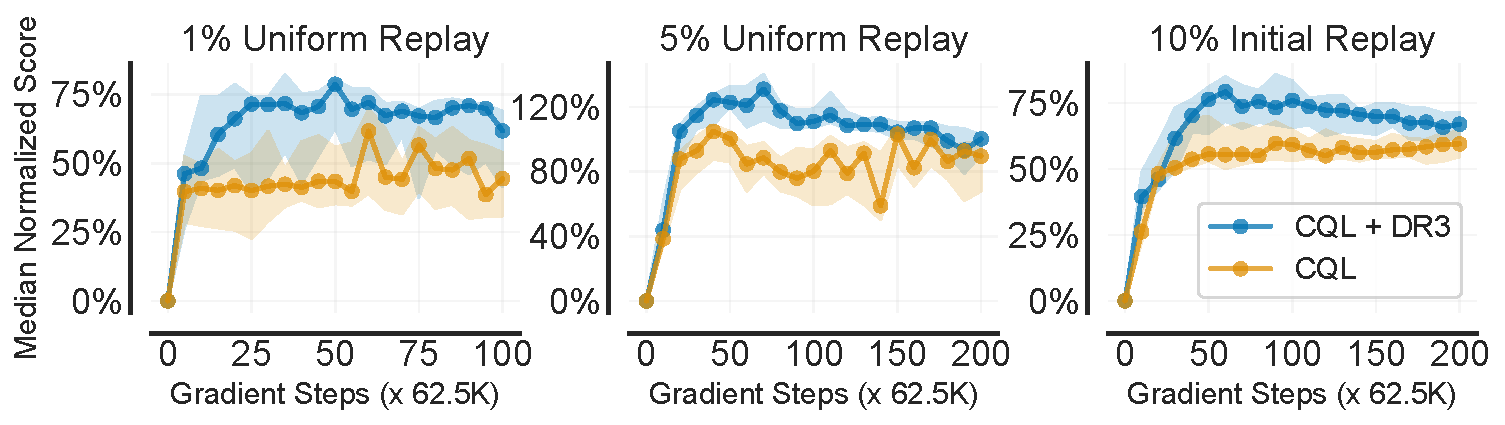
\includegraphics[width=\linewidth]{figures/atari_new/Median_cql_penalty.pdf}
%     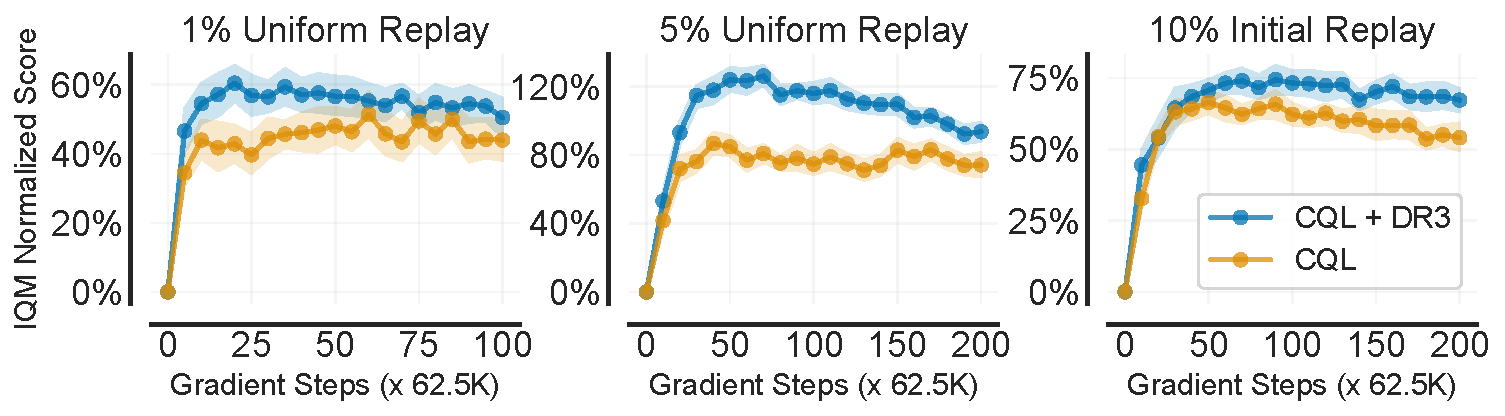
\includegraphics[width=\linewidth]{figures/atari_new/IQM_cql_penalty.pdf}
%     % 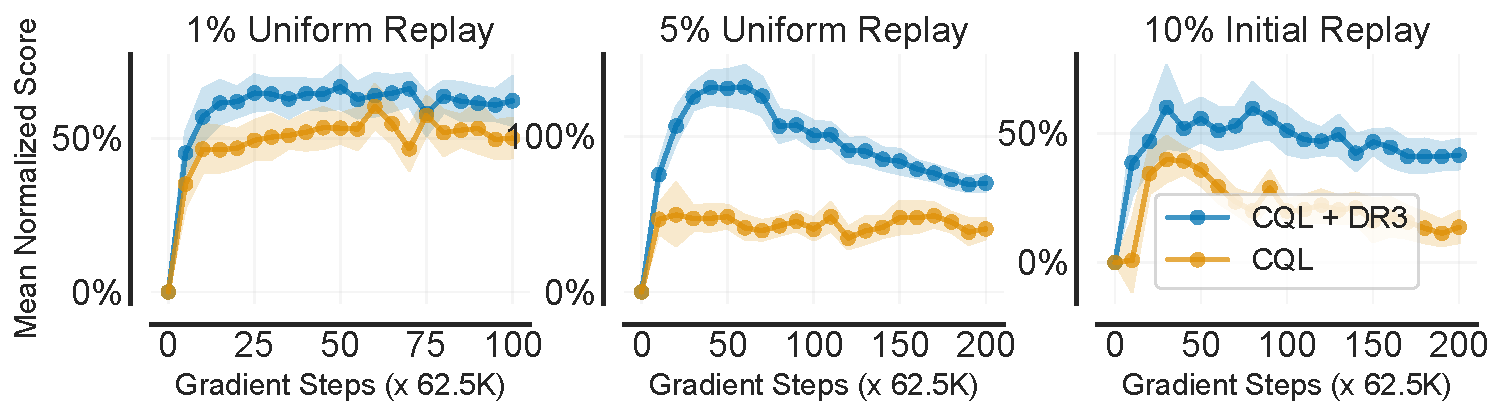
\includegraphics[width=\linewidth]{figures/atari_new/Mean_cql_penalty.pdf}
%     % 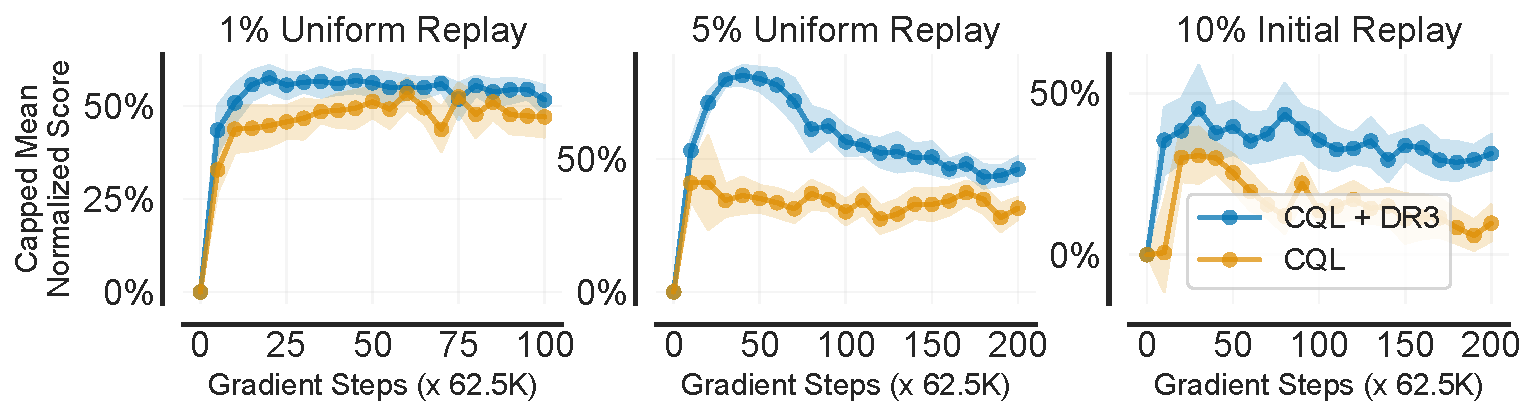
\includegraphics[width=\linewidth]{figures/atari_new/Capped_Mean_cql_penalty.pdf}
%     \vspace{-0.65cm}
%     \caption{Behavior Normalized Scores across 17 Atari games. We use Interquartile mean~(IQM).}
%     \label{fig:atari_5_percent}
% \end{figure*}



% \begin{figure}[t]
%     \centering
%     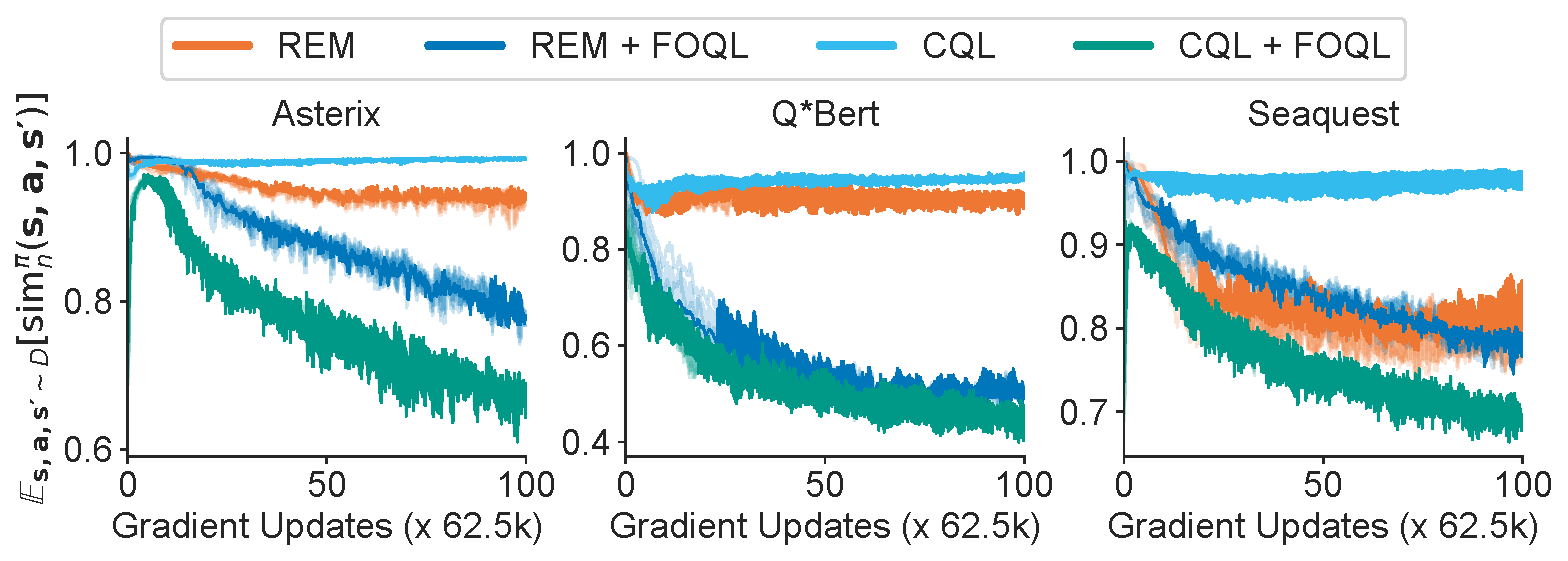
\includegraphics[width=\linewidth]{atari/norm_3_games_cql_rem.pdf}
%     \vspace{-0.65cm}
%     \caption{In addition to minimizing unnormalized similarities~($\simunnorm(\bs, \ba, \bs')$), \methodname\ attains much lower normalized similarities as compared to CQL and REM. The results are shown for training with 5\% DQN replay dataset averaged over 5 seeds.}\label{fig:atari_3_cosine}
%     \vspace{-0.5cm}
% \end{figure}


% \begin{figure*}[t]
%     \centering
%     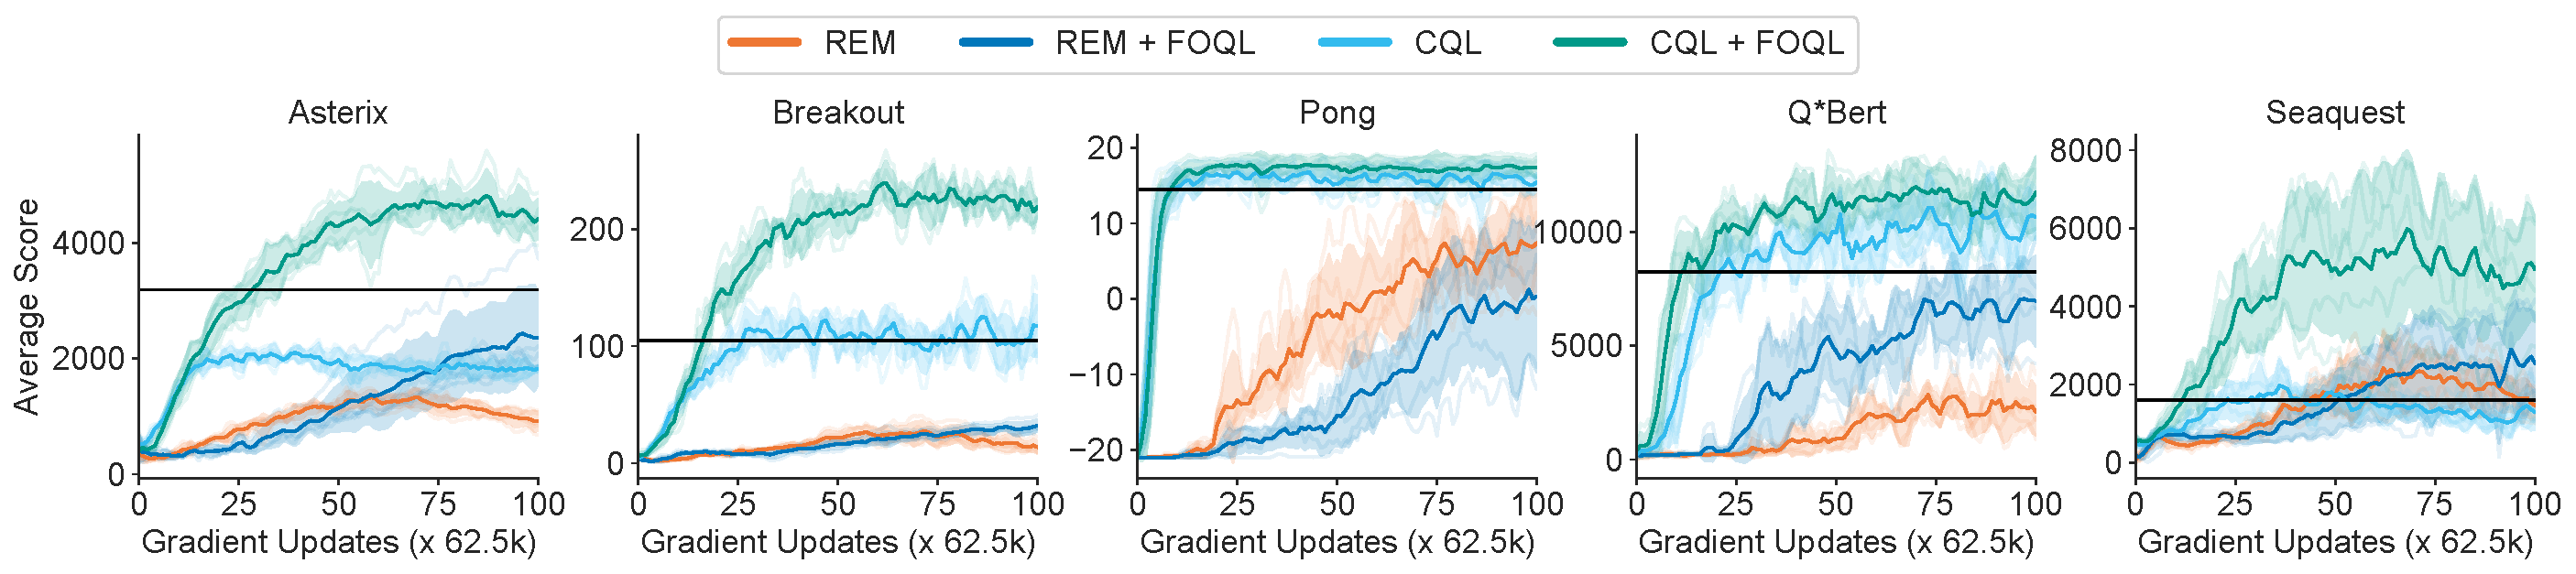
\includegraphics[width=\linewidth]{atari/5_percent_res_100.pdf}
%     \vspace{-0.65cm}
%     \caption{Evaluation performance of offline REM and CQL with and without \methodname\ on the 5\% DQN replay dataset~\citep{agarwal2019optimistic}. Note that the data collected during evaluation is not provided to offline agents during training. The horizontal line shows the average performance of the trajectories in entire DQN replay dataset. \methodname\ substantially improves the performance of CQL and REM as well as prevents the decay in performance of REM with more gradient updates on \textsc{Seaquest} and \textsc{Asterix}. For \textsc{Pong}, training for longer~(12.5 million updates) results in improved score for REM + \methodname\ over REM.}
%     \label{fig:atari_5_percent}
% \end{figure*}


% \begin{table*}[t]
%     \centering
%     \caption{Normalized returns on sub-sampled Atari DQN Replay datasets~\citep{agarwal2019optimistic}. A random policy is provided a normalized score of zero while the average performance of the trajectories in the entire DQN replay dataset is assigned a normalized score of 100. We report results based on 6.5 million gradient updates with batch size of 32 for the 1\% setting and 12.5 million gradient updates for the 5\% and 10\% settings. The individual scores and learning curves for all the 17 games are provided in the Appendix~\ref{app:atari_results}.}
%     \label{tab:cql_res}
%     \vspace{0.2cm}
% \begin{tabular}{cccccc}
% \toprule
% %%AK.1.26: maybe we want to name the average performance as Stability coefficient or something like that but thats a minor point
% \multirow{2}{*}{DQN Replay Setting} & Normalized Score Metric & \multicolumn{2}{c}{Average Performance}   & \multicolumn{2}{c}{Maximum Performance} \\
% & (17 games) & CQL & CQL + \methodname & CQL & CQL + \methodname \\
% \midrule
% 1\% replay &  Median & 43.3 & \textbf{71.0} & 73.2 & \textbf{96.3} \\
% (uniformly sampled) & Mean & 50.7 & \textbf{60.9} & 74.4 & \textbf{84.6}  \\
% \midrule
% {5\% replay} & Median  & 84.6 & \textbf{104.9} & 127.8 & \textbf{150.7} \\
% (uniformly sampled)  & Mean & 43.3 & \textbf{97.2} &  139.5 & \textbf{189.5}  \\
% \midrule
% {10\% replay} & Median  & 53.4 &  \textbf{69.9} & 73.3 & \textbf{97.2} \\
% (initial exploration data) & Mean & 21.8 & \textbf{49.6} &  79.4 & \textbf{140.0}  \\
% \bottomrule
% \end{tabular}
% \end{table*}

%% Final Performance CQL vs Penalty
% -----DR3+CQL-----
% *****Median*****
% 1% data
% Median 61.8 [41.6 69. ]
% 5% data
% Median 100.2 [ 90.6 102.7]
% 10% data
% Median 67.0 [62.1 71.4]
% *****IQM*****
% 1% data
% IQM 50.5 [44.9 56.1]
% 5% data
% IQM 93.6 [88. 99.]
% 10% data
% IQM 67.3 [63.2 71.4]
% -----CQL-----
% *****Median*****
% 1% data
% Median 44.4 [30.9 54. ]
% 5% data
% Median 89.6 [67.9 98.2]
% 10% data
% Median 59.6 [54.6 64.4]
% *****IQM*****
% 1% data
% IQM 44.0 [38.1 49.8]
% 5% data
% IQM 74.2 [67.3 81.4]
% 10% data
% IQM 54.1 [49.5 59.3]

%% Final performance REM vs REM+penalty
% -----DR3+REM-----
% *****Median*****
% 1% data
% Median 13.1 [10.  18.4]
% 5% data
% Median 72.4 [65.7 81.1]
% 10% data
% Median 72.4 [65.7 81.1]
% *****IQM*****
% 1% data
% IQM 13.4 [11.  16.4]
% 5% data
% IQM 77.2 [71.4 83.9]
% 10% data
% IQM 77.2 [71.4 83.9]
% -----REM-----
% *****Median*****
% 1% data
% Median -0.0 [-0.7  0.1]
% 5% data
% Median 24.9 [14.5 29. ]
% 10% data
% Median 24.9 [14.5 29. ]
% *****IQM*****
% 1% data
% IQM -0.1 [-0.7  0.6]
% 5% data
% IQM 23.5 [19.9 27.3]
% 10% data
% IQM 23.5 [19.9 27.3]


% REM vs REM + penalty Average performance (stability)
% -----DR3+REM-----
% *****Median*****
% 1% data
% Median 11.7
% 5% data
% Median 52.5
% 10% data
% Median 63.9
% *****IQM*****
% 1% data
% IQM 12.4
% 5% data
% IQM 53.5
% 10% data
% IQM 67.8
% -----REM-----
% *****Median*****
% 1% data
% Median 3.1
% 5% data
% Median 18.8
% 10% data
% Median 47.7
% *****IQM*****
% 1% data
% IQM 3.4
% 5% data
% IQM 21.1
% 10% data
% IQM 47.9

% FInal performance (scaled via random scores and CQL is 100\% for IUP comparison):
% Asterix 256.6
% BeamRider 18.6
% Breakout 176.3
% DemonAttack 228.0
% DoubleDunk 133.5
% Enduro 115.2
% IceHockey 51.7
% Jamesbond 310.8
% MsPacman 131.5
% Pong 105.5
% Qbert 114.4
% RoadRunner 100.0
% Seaquest 366.6
% SpaceInvaders 322.8
% WizardOfWor 80.3
% YarsRevenge 75.7
% Zaxxon 485.6



% \begin{table*}[t]
%     \centering
%     \caption{Normalized returns on sub-sampled Atari DQN replay datasets~\citep{agarwal2019optimistic}. The individual scores and learning curves for all the 17 games are provided in the Appendix~\ref{app:atari_results}. When combined with REM, we used a coefficient of $\alpha = 0.001$ to show the robustness of \methodname\ across different datasets. \color{red}{Merge the two tables somehow to save space.}}
%     \label{tab:rem_res}
%     \vspace{0.2cm}
% \begin{tabular}{cccccc}
% \toprule
% %%AK.1.26: maybe we want to name the average performance as Stability coefficient or something like that but thats a minor point
% \multirow{2}{*}{DQN Replay Setting} & Normalized Score Metric & \multicolumn{2}{c}{Average Performance}   & \multicolumn{2}{c}{Maximum Performance} \\
% & (17 games) & REM & REM + \methodname & REM & REM + \methodname \\
% \midrule
% 1\% replay &  Median & 4.7 & \textbf{19.3} & 25.5 & \textbf{42.5} \\
% (uniformly sampled) & Mean & -1.8 & \textbf{47.2} &  72.4 & \textbf{100.2}  \\
% \midrule
% {5\% replay} & Median  & 27.4 & \textbf{58.5} & 88.8 & \textbf{99.8} \\
% (uniformly sampled)  & Mean & 40.9 & \textbf{84.7} &  141.1 & \textbf{165.8}  \\
% \midrule
% {10\% replay} & Median  & 50.7 &  \textbf{68.5} & 107 & \textbf{108.5} \\
% (initial exploration data) & Mean & 63.7 & \textbf{84.4} &  136.5 & \textbf{140.7}  \\
% \bottomrule
% \end{tabular}
% \end{table*}

%% Final Performance CQL vs Penalty
% -----DR3+CQL-----
% *****Median*****
% 1% data
% Median 61.8 [41.6 69. ]
% 5% data
% Median 100.2 [ 90.6 102.7]
% 10% data
% Median 67.0 [62.1 71.4]
% *****IQM*****
% 1% data
% IQM 50.5 [44.9 56.1]
% 5% data
% IQM 93.6 [88. 99.]
% 10% data
% IQM 67.3 [63.2 71.4]
% -----CQL-----
% *****Median*****
% 1% data
% Median 44.4 [30.9 54. ]
% 5% data
% Median 89.6 [67.9 98.2]
% 10% data
% Median 59.6 [54.6 64.4]
% *****IQM*****
% 1% data
% IQM 44.0 [38.1 49.8]
% 5% data
% IQM 74.2 [67.3 81.4]
% 10% data
% IQM 54.1 [49.5 59.3]

% CQL  vs CQL + penalty Average performance (stability)
% -----DR3+CQL-----
% *****Median*****
% 1% data
% Median 63.7
% 5% data
% Median 102.6
% 10% data
% Median 65.2
% *****IQM*****
% 1% data
% IQM 52.6
% 5% data
% IQM 102.4
% 10% data
% IQM 65.2
% -----CQL-----
% *****Median*****
% 1% data
% Median 42.5
% 5% data
% Median 81.4
% 10% data
% Median 52.1
% *****IQM*****
% 1% data
% IQM 42.8
% 5% data
% IQM 72.3
% 10% data
% IQM 56.3


% \begin{table*}[t]
%     \centering
%     \caption{\small{Performance of REM, REM + \methodname after 6.5M gradient steps for the 1\% setting and 12.5M gradient steps for the 5\%, 10\% settings. Individual scores for all 17 games are provided in the Appendix~\ref{app:atari_results}.}}
%     \label{tab:rem_res}
%     \vspace{0.2cm}
% \begin{tabular}{cccccc}
% \toprule
% \multirow{2}{*}{\textbf{Data}} & \textbf{Metric} & \multicolumn{2}{c}{\textbf{Last iteration score}}   & \multicolumn{2}{c}{\textbf{Stability score}} \\
% & (17 games) & REM & REM + \methodname & REM & REM + \methodname \\
% \midrule
% 1\% &  Median & 0.0 & \textbf{13.1} & 3.1 & \textbf{11.7} \\
%  & IQM & -0.1 & \textbf{13.4} & 3.4 & \textbf{12.4}  \\
% \midrule
% 5\% & Median  & 24.9 & \textbf{72.4} & 18.8 & \textbf{52.5} \\
%  & IQM & 23.5 & \textbf{77.2} &  21.1 & \textbf{53.5}  \\
% \midrule
% 10\% & Median & 24.9 &  \textbf{72.4} & 47.7 & \textbf{63.9} \\
%  & IQM & 23.5 & \textbf{77.4} &  47.9 & \textbf{67.8}  \\
% \bottomrule
% \end{tabular}
% \end{table*}



% REM vs REM + penalty Average performance (stability)
% -----DR3+REM-----
% *****Median*****
% 1% data
% Median 11.7
% 5% data
% Median 52.5
% 10% data
% Median 63.9
% *****IQM*****
% 1% data
% IQM 12.4
% 5% data
% IQM 53.5
% 10% data
% IQM 67.8
% -----REM-----
% *****Median*****
% 1% data
% Median 3.1
% 5% data
% Median 18.8
% 10% data
% Median 47.7
% *****IQM*****
% 1% data
% IQM 3.4
% 5% data
% IQM 21.1
% 10% data
% IQM 47.9

%% Final performance REM vs REM+penalty
% -----DR3+REM-----
% *****Median*****
% 1% data
% Median 13.1 [10.  18.4]
% 5% data
% Median 72.4 [65.7 81.1]
% 10% data
% Median 72.4 [65.7 81.1]
% *****IQM*****
% 1% data
% IQM 13.4 [11.  16.4]
% 5% data
% IQM 77.2 [71.4 83.9]
% 10% data
% IQM 77.2 [71.4 83.9]
% -----REM-----
% *****Median*****
% 1% data
% Median -0.0 [-0.7  0.1]
% 5% data
% Median 24.9 [14.5 29. ]
% 10% data
% Median 24.9 [14.5 29. ]
% *****IQM*****
% 1% data
% IQM -0.1 [-0.7  0.6]
% 5% data
% IQM 23.5 [19.9 27.3]
% 10% data
% IQM 23.5 [19.9 27.3]

% \begin{table*}[t]
%     \centering
%     \caption{\small{Performance of REM, REM + \methodname after 6.5M gradient steps for the 1\% setting and 12.5M gradient steps for the 5\%, 10\% settings. Individual scores for all 17 games are provided in the Appendix~\ref{app:atari_results}.}}
%     \label{tab:rem_res}
%     \vspace{0.2cm}
% \begin{tabular}{cccccc}
% \toprule
% \multirow{2}{*}{\textbf{Data}} & \textbf{Metric} & \multicolumn{2}{c}{\textbf{Last iteration score}}   & \multicolumn{2}{c}{\textbf{Stability score}} \\
% & (17 games) & REM & REM + \methodname & REM & REM + \methodname \\
% \midrule
% 1\% &  Median & 0.0 & \textbf{13.1} & 3.1 & \textbf{11.7} \\
%  & IQM & -0.1 & \textbf{13.4} & 3.4 & \textbf{12.4}  \\
% \midrule
% 5\% & Median  & 24.9 & \textbf{72.4} & 18.8 & \textbf{52.5} \\
%  & IQM & 23.5 & \textbf{77.2} &  21.1 & \textbf{53.5}  \\
% \midrule
% 10\% & Median & 24.9 &  \textbf{72.4} & 47.7 & \textbf{63.9} \\
%  & IQM & 23.5 & \textbf{77.4} &  47.9 & \textbf{67.8}  \\
% \bottomrule
% \end{tabular}
% \end{table*}

% \begin{wrapfigure}{r}{0.57\textwidth}
%     \centering
%     \vspace{-5pt}
%     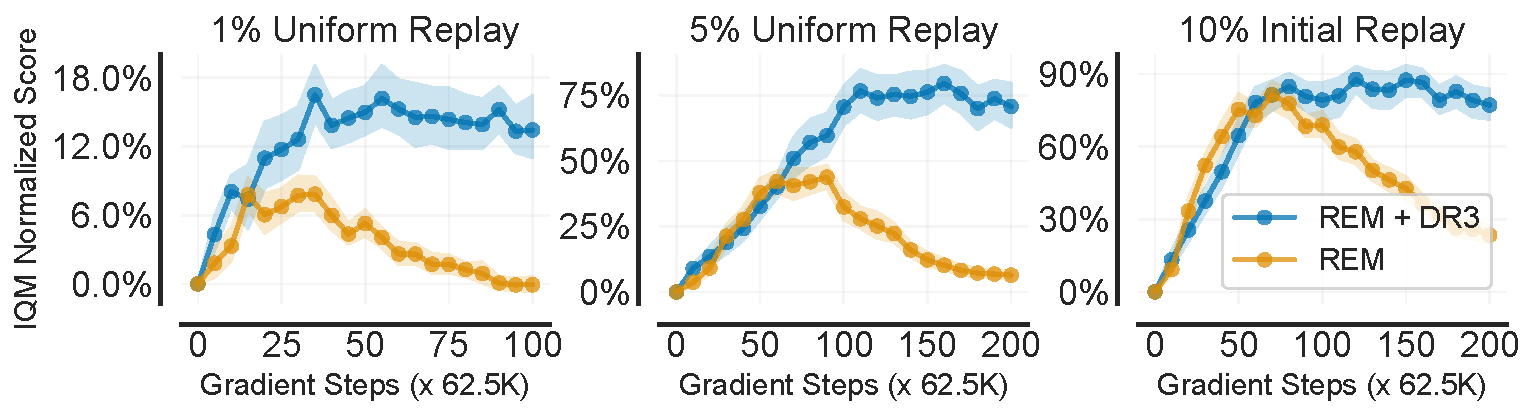
\includegraphics[width=0.99\linewidth]{figures/atari_new/IQM_rem_penalty.pdf}
%     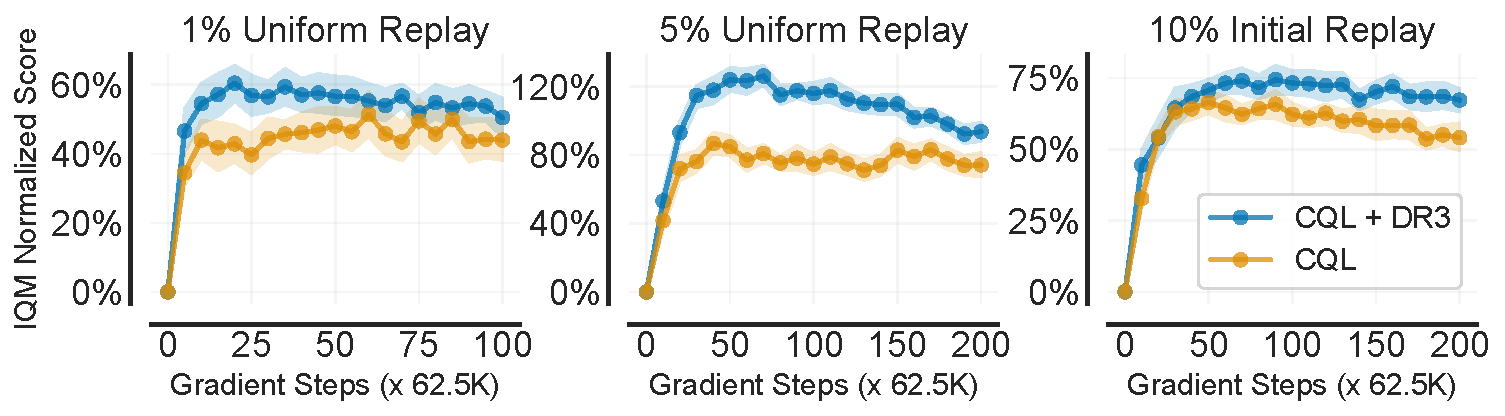
\includegraphics[width=0.99\linewidth]{figures/atari_new/IQM_cql_penalty.pdf}
%     \vspace{-0.25in}
%     \caption{\small{\textbf{Average normalized performance across 17 Atari games for REM + \methodname\ (top), CQL + \methodname\ (bottom)} over the course of training with different datasets. x-axis represents \emph{gradient steps}; no new data is collected. While na\"ive REM suffers from a degradation in performance with more training, REM + \methodname\ not only remains generally stable with more training, but also attains higher final performance. CQL + \methodname\ attains higher performance than CQL. As recommended by \citet{agarwal2021precipice}, we report interquartile Mean (IQM) with stratified bootstrap 95\% CIs as shaded regions.}}
%     \label{fig:atari_all_combined}
%     \vspace{-0.45cm}
% \end{wrapfigure}
\textbf{{Offline RL on Atari 2600 games.}} We compare \methodname\ to prior offline RL methods on a set of offline Atari datasets of varying sizes and quality, akin to \citet{agarwal2019optimistic, kumar2021implicit}. We evaluated on three datasets: \textbf{(1)} 1\% and 5\% samples drawn uniformly at random from DQN replay; \textbf{(2)} a dataset with more suboptimal data consisting of the first 10\% samples observed by an online DQN. Following \citet{agarwal2021precipice}, we report the interquartile mean~(IQM) normalized scores across 17 games over the course of training in Figure~\ref{fig:atari_all_combined} and report the IQM average performance in Table~\ref{tab:cql_res}. Observe that combining \methodname\ with modern offline RL methods (CQL, REM) attains the best final and average performance across the 17 Atari games tested on, directly improving upon prior methods
across all the datasets. When \methodname\ is used in conjunction with REM, it prevents {severe} unlearning and performance degradation with more training. CQL + \methodname\ improves by \textbf{20\%} over CQL on final performance and attains \textbf{25\%} better average performance. {While DR3 is not unequivocally ``stable'', as its performance also degrades relative to the peak it achieves (Figure~\ref{fig:atari_all_combined}), it is more stable relative to base offline RL algorithms.} We also compare \methodname\ to the $\mathrm{srank}(\Phi)$ penalty proposed to counter rank collapse~\citep{kumar2021implicit}. Directly taking median normalized score improvements reported by \citet{kumar2021implicit}, CQL + \methodname\ improves by over \textbf{2x} (31.5\%) over na\"ive CQL relative to the srank penalty~(14.1\%), indicating DR3's efficacy.
% this $\text{srank}$ penalty only attains a median improvement of 14.1\% over na\"ive CQL, whereas CQL + \methodname\ attains a median improvement of \textbf{31.5\%} over CQL. Thus, CQL + \methodname\ improves by over \textbf{2x} relative to the srank penalty, indicating DR3's efficacy.
% This indicates that by directly addressing the adverse impacts of implicit regularization, \methodname\ can substantially improve upon prior methods that only address its symptoms.  

%Notably, REM performs similar to a random policy in terms of average performance on the 1\%  setting, which is significantly improved by \methodname.
%%SL.2.1: I think we can cut this last sentence, and instead focus on the more positive takeaways.

% To evaluate whether the improvements from \methodname\ stem from penalizing unnormalized similarities $\simunnorm(\bs, \ba, \bs')$, we also compare \methodname\ to penalizing (1) $\simnorm(\bs, \ba, \bs')$, or (2) feature norms~($\|\phi(\bs)\|_2$) on the 5\% dataset on 5 games. The full results, shown in Appendix~\ref{}, confirms that both of these penalties perform substantially worse than \methodname, aligned with our theoretical analysis about effectiveness of \methodname~(Section~\ref{sec:method_analysis}).

%%SL.2.1: This last phrase is without context. What question is it trying to answer? What is the motivation? Start with a sentence of motivation or a question, then evidence, then answer. Something like: Is [whatever] true? To answer this question, we can [do something]. The full results, shown in [where], indicate [something]. This suggests that [something].
\begin{wrapfigure}{r}{0.42\textwidth}
\small \begin{center}
\vspace{-30pt}
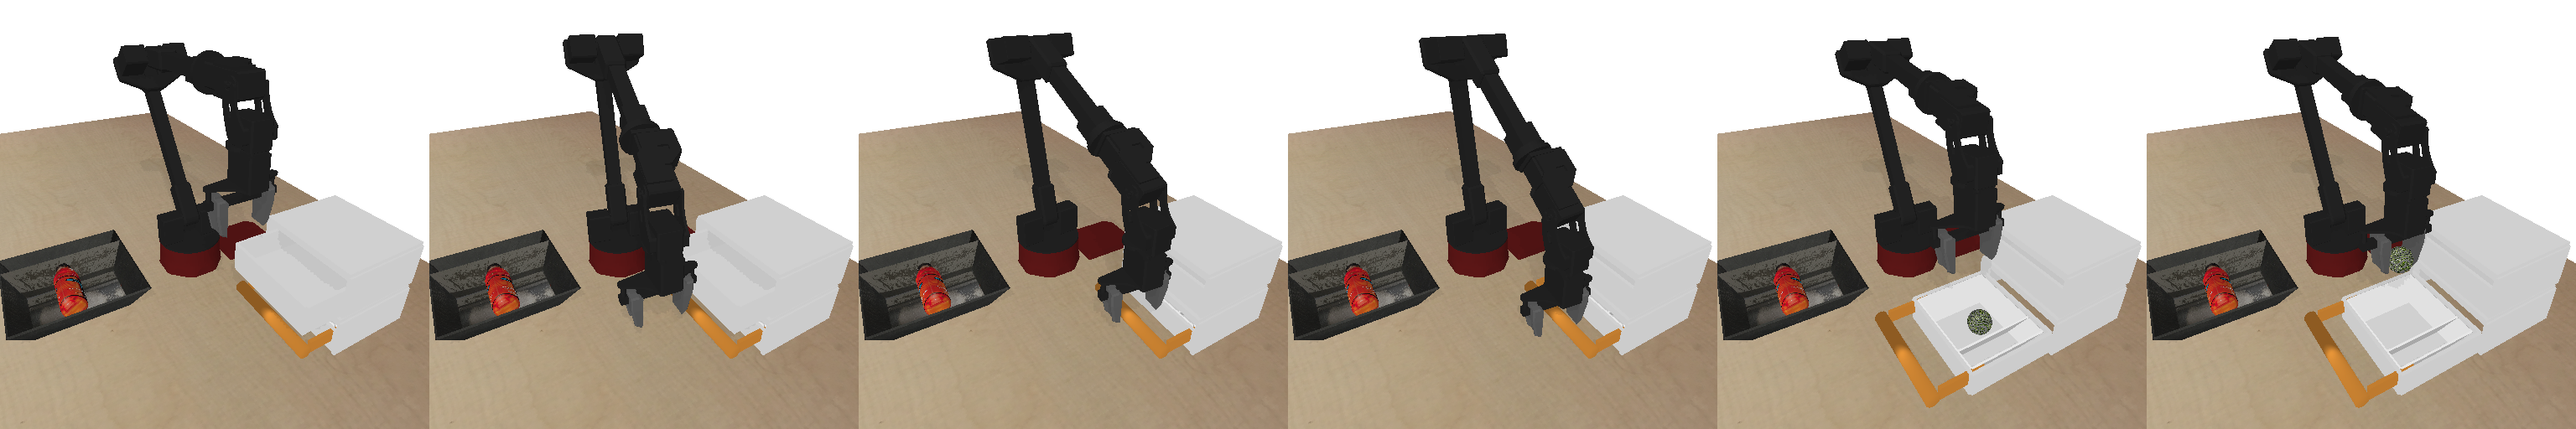
\includegraphics[width=0.99\linewidth]{figures/close_open_grasp (1).png}
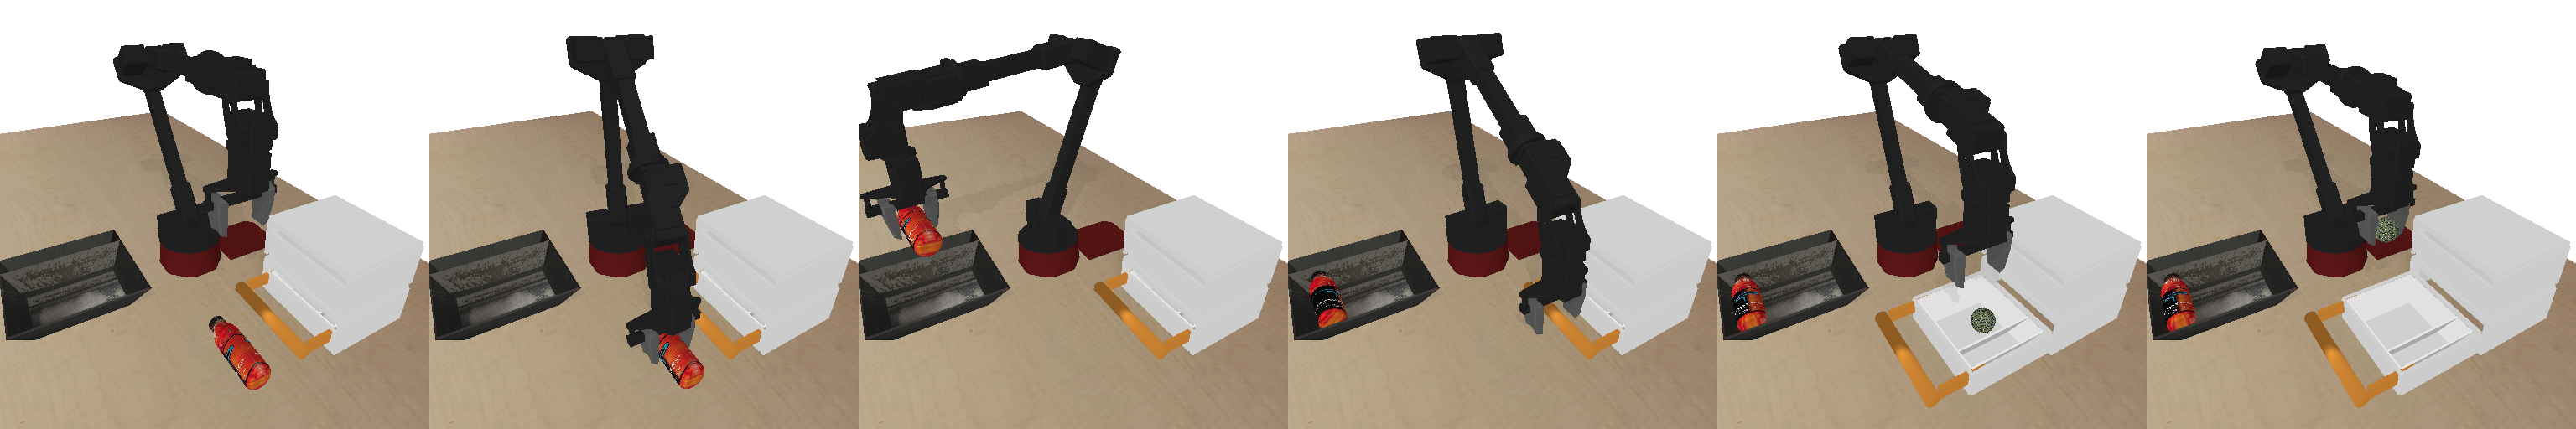
\includegraphics[width=0.99\linewidth]{figures/pickplace_open_grasp.png}
\vspace{-20pt}
\end{center}
\end{wrapfigure}
\textbf{{Offline RL on robotic manipulation from}} \textbf{{images.}} Next, we aim to evaluate the efficacy of \methodname\ on two image-based robotic manipulation tasks~\citep{singh2020cog}~(visualized on the right) that require composition of skills (e.g., opening a drawer, closing a drawer, picking an obstructive object, placing an object, etc.) over extended horizons using only a sparse 0-1 reward. 
As shown in Figure~\ref{fig:cog_figure}, combining \methodname\ with COG improves over COG.

\begin{table}[t]
    \centering
\fontsize{8}{8}\selectfont
    \centering
    \vspace{-0.2cm}
    \caption{\footnotesize{IQM normalized average performance (training stability) across 17 games, with 95\% CIs in parenthesis, after 6.5M gradient steps for the 1\% setting and 12.5M gradient steps for the 5\%, 10\% settings. Individual performances reported in Tables~\ref{tab:cql_dqn_1}-\ref{tab:rem_dqn_10}. \methodname\ improves the stability over both CQL and REM.  }}%As recommended by \citet{agarwal2021precipice}, we report IQM with 95\% CIs.}
    \label{tab:cql_res}
    \vspace{-0.1cm}
\begin{tabular}{lcccc}
\toprule
% \multirow{2}{*}{\textbf{Data}}  & \multicolumn{4}{c}{\textbf{Stability performance}} \\
Data & CQL & CQL + \methodname & REM & REM + \methodname \\
\midrule
1\%   & 43.7~\ss{(39.6, 48.6)} & \textbf{56.9}~\ss{(52.5, 61.2)} & 4.0~\ss{(3.3, 4.8)} & \textbf{16.5}~\ss{(14.5, 18.6)}  \\
\midrule
5\%   &  78.1~\ss{(74.5, 82.4)} & \textbf{105.7}~\ss{(101.9, 110.9)} & 25.9~\ss{(23.4, 28.8)} & \textbf{60.2}~\ss({55.8, 65.1}) \\
\midrule
10\%  & 59.3~\ss{(56.4, 61.9)} & \textbf{65.8}~\ss{(63.3, 68.3)} & 53.3~\ss{(51.4, 55.3)} & \textbf{73.8}~\ss{(69.3, 78)} \\
\bottomrule
\vspace{-0.25in}
\end{tabular}
\end{table}

\begin{figure}[t]
% \vspace{-pt}
\centering
\begin{minipage}{.4\textwidth}
% 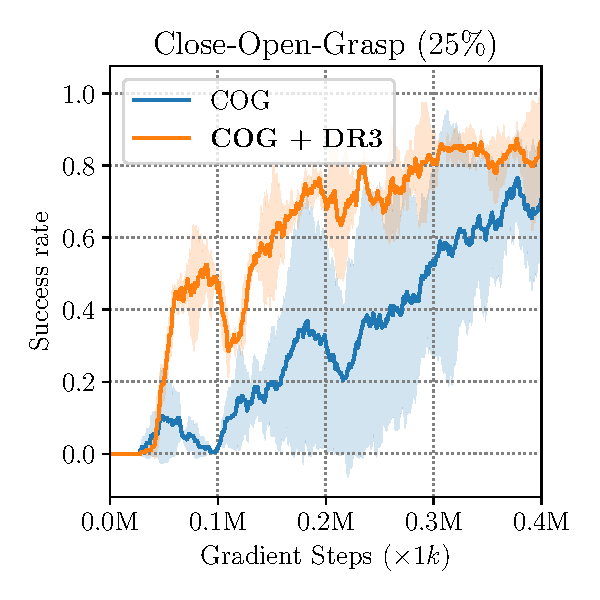
\includegraphics[width=0.49\linewidth]{figures/Widow250DoubleDrawerCloseOpenGraspNeutral-v0_cog_vs_dr3_25_v2.pdf}
% 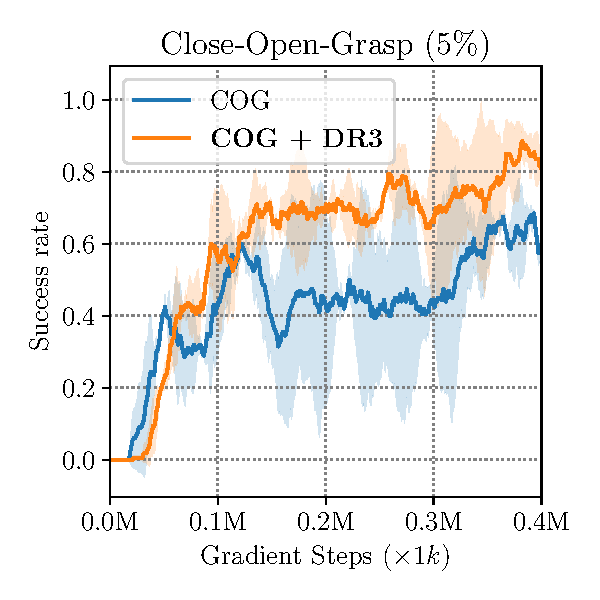
\includegraphics[width=0.49\linewidth]{figures/Widow250DoubleDrawerCloseOpenGraspNeutral-v0_cog_vs_dr3_25_v3.pdf}
% 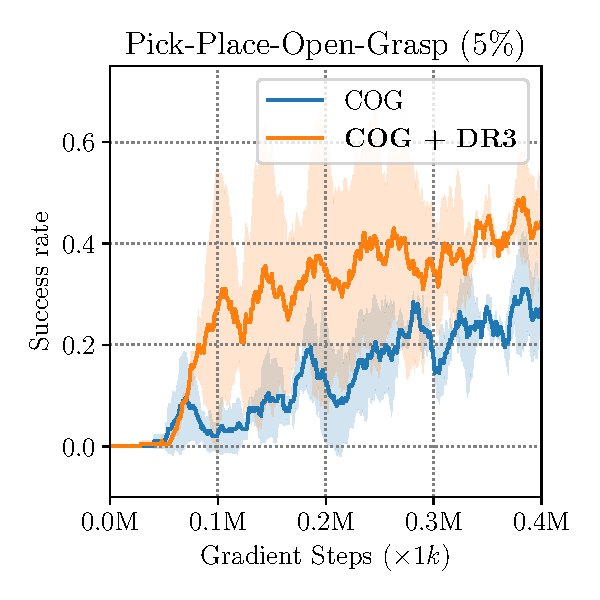
\includegraphics[width=0.49\linewidth]{figures/Widow250DoubleDrawerPickPlaceOpenGraspNeutral-v0_cog_vs_dr3_25_v4.pdf}
% 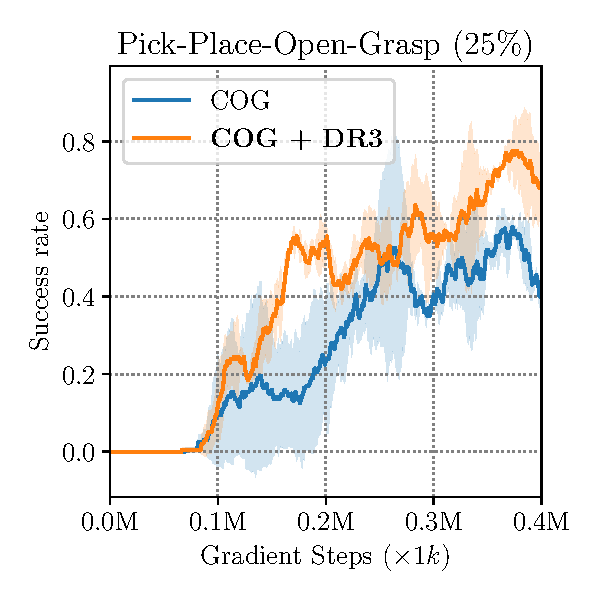
\includegraphics[width=0.49\linewidth]{figures/Widow250DoubleDrawerPickPlaceOpenGraspNeutral-v0_cog_vs_dr3_25.pdf}
% \vspace{-10pt}
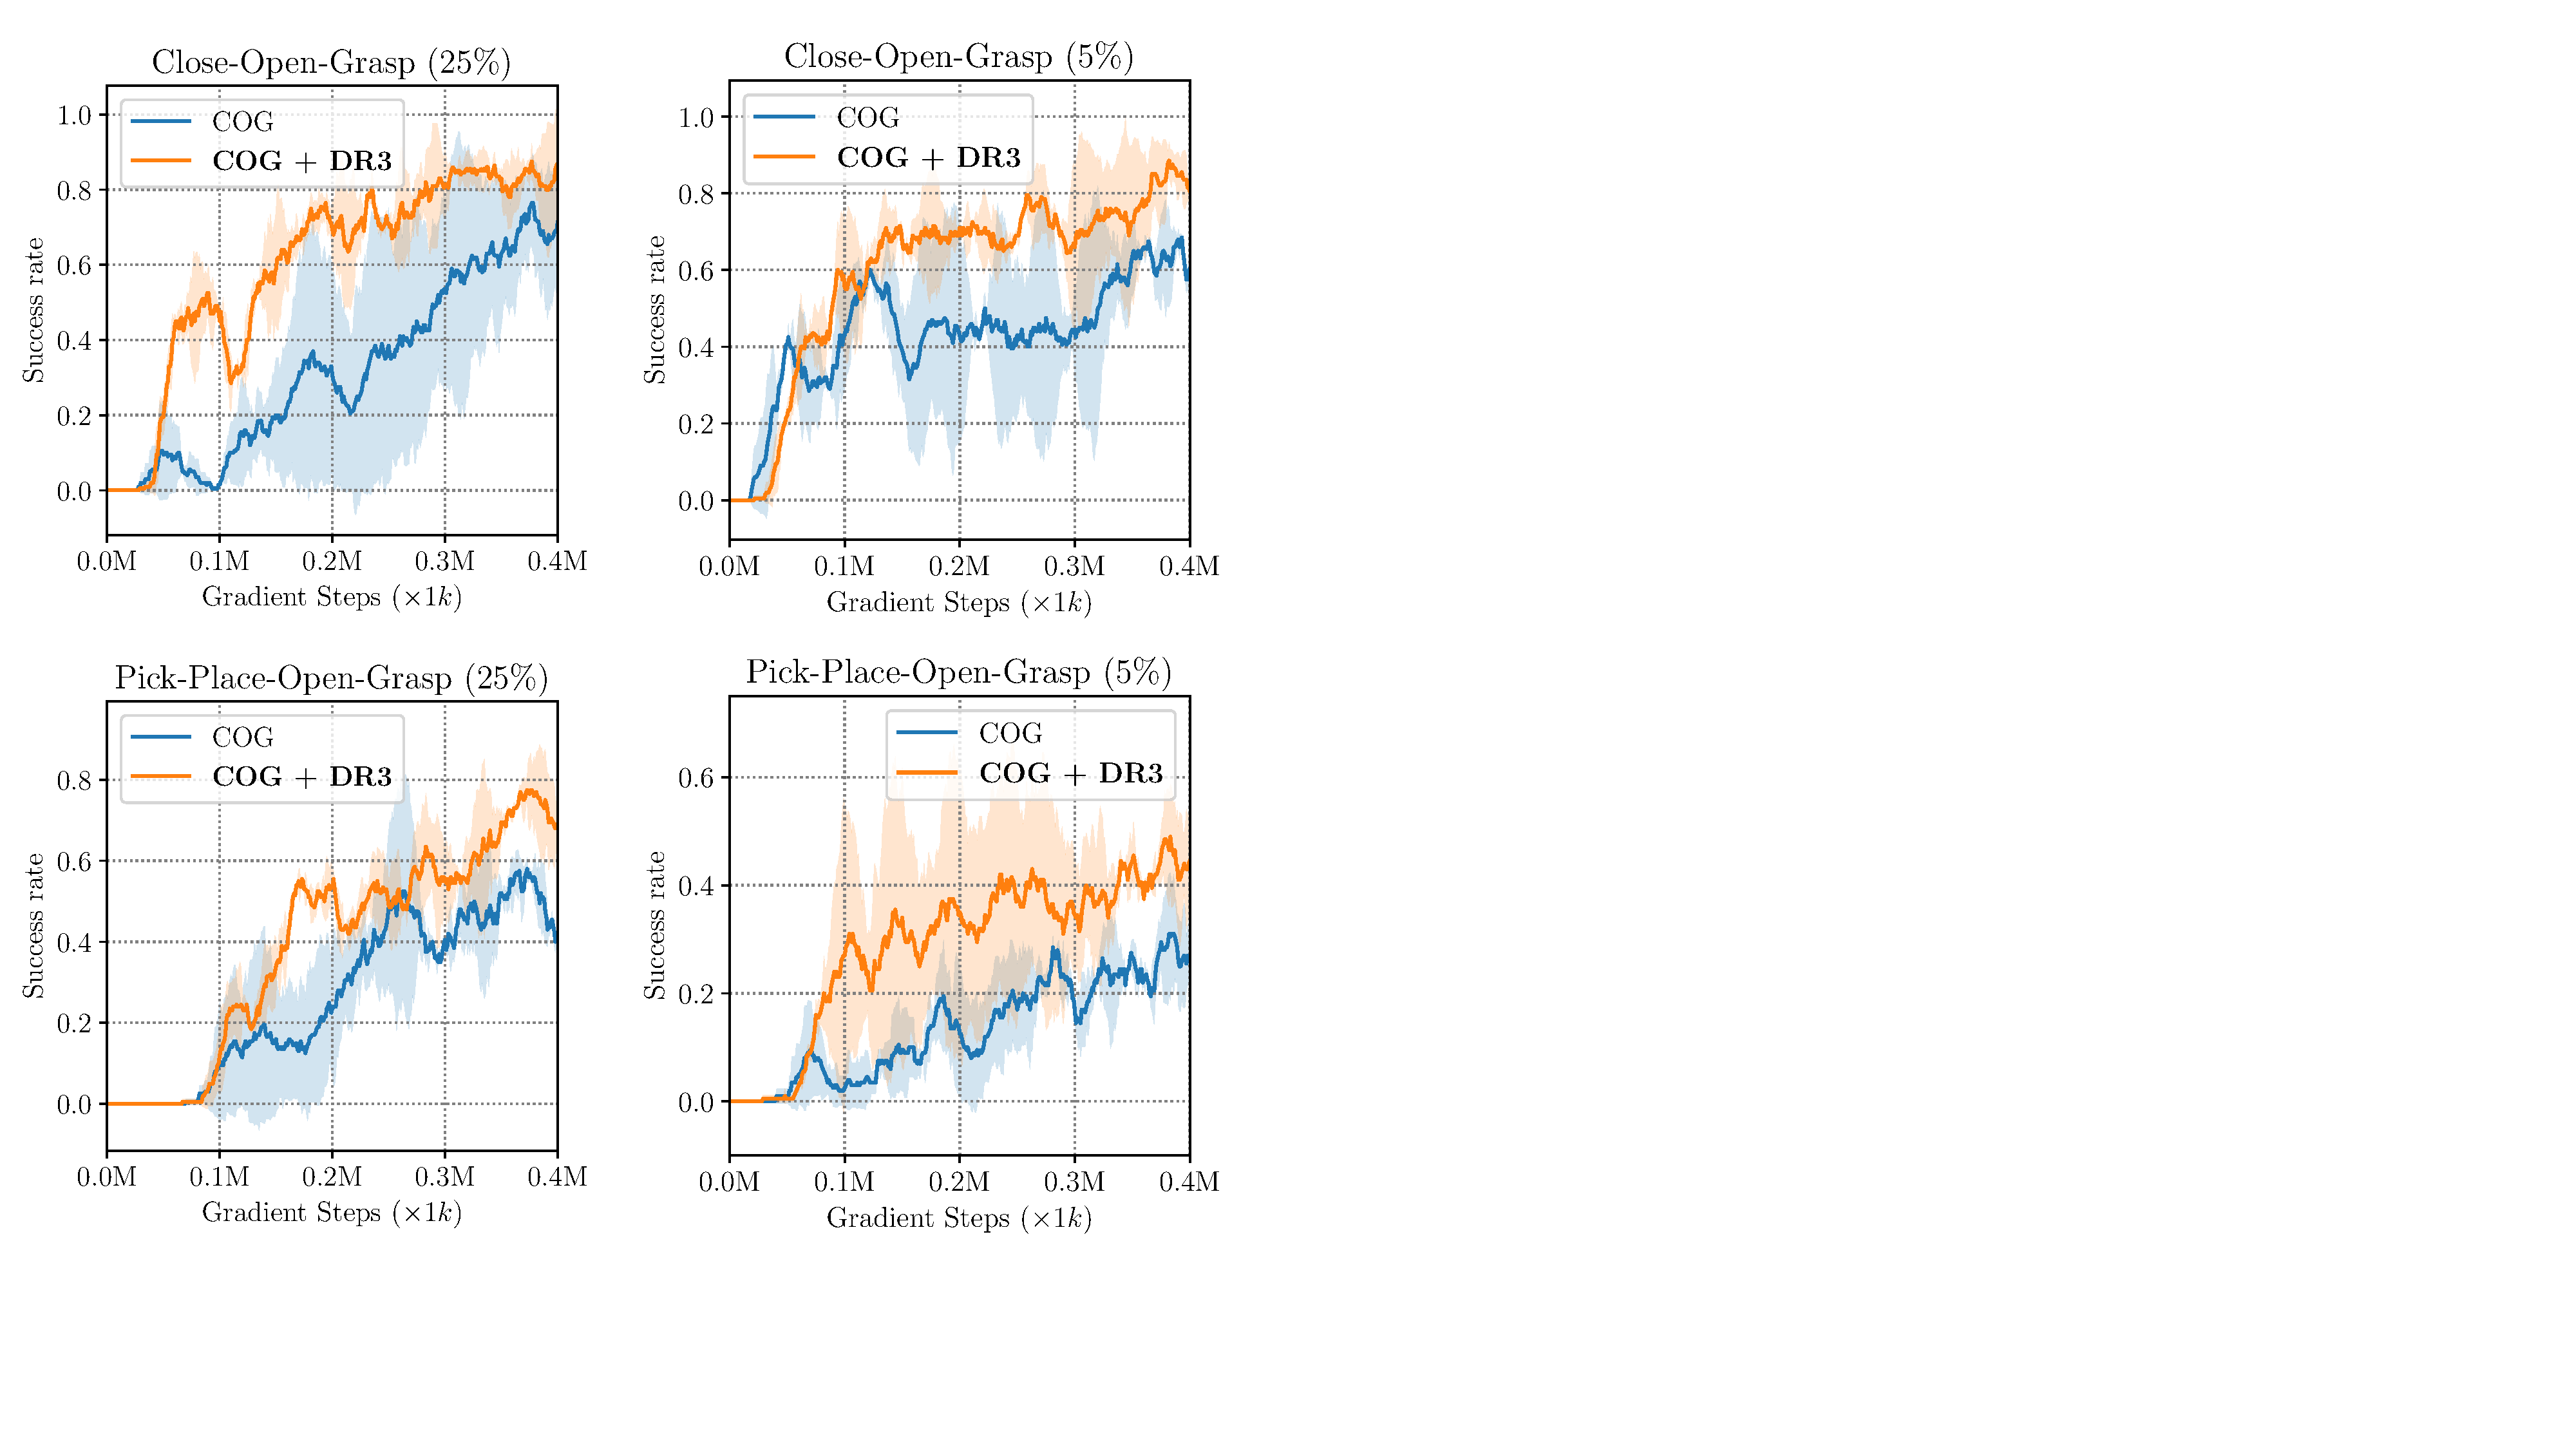
\includegraphics[width=0.96\linewidth]{figures/cog_plots.pdf}
\vspace{-0.2cm}
\caption{\footnotesize{\textbf{Performance of \methodname\ + COG} on two manipulation tasks using only 5\% and 25\% of the data used by \citet{singh2020cog} to make these more challenging.
COG + \methodname\  outperforms COG in training and attains higher average and final performance.}}
\label{fig:cog_figure}
\end{minipage}~~\vline~~
\begin{minipage}{.56\textwidth}
    \centering
    % \vspace{-0.1in}
    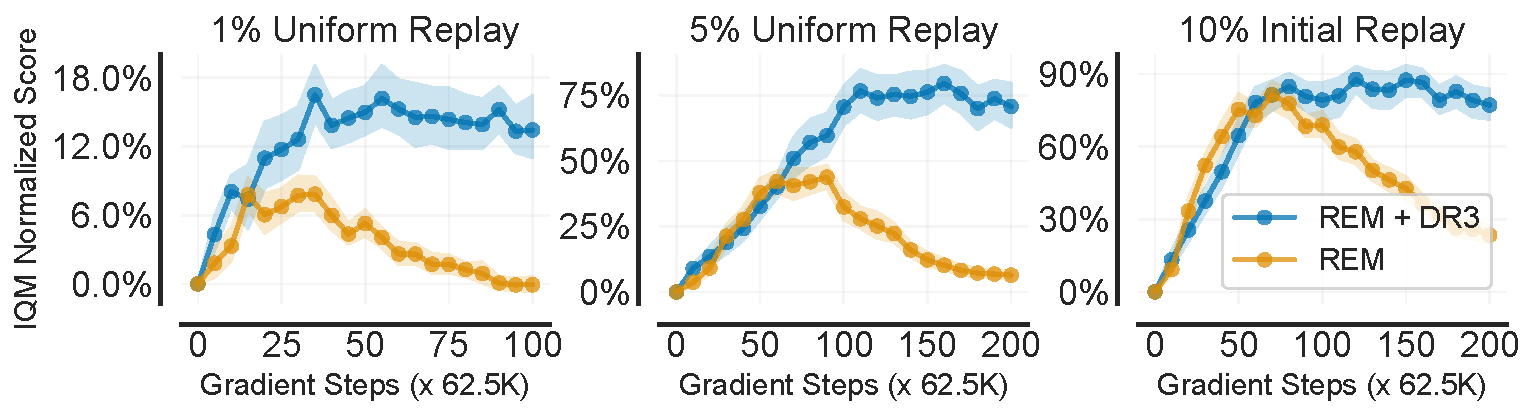
\includegraphics[width=0.99\linewidth]{figures/atari_new/IQM_rem_penalty.pdf}
    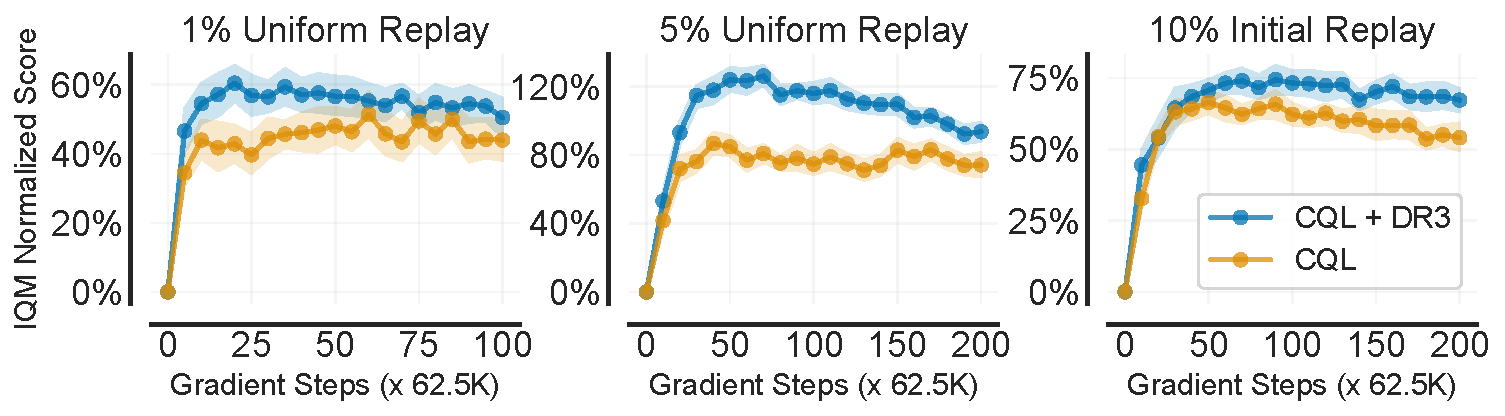
\includegraphics[width=0.99\linewidth]{figures/atari_new/IQM_cql_penalty.pdf}
    \vspace{-0.25in}
    \caption{\footnotesize{\textbf{Normalized performance across 17 Atari games for REM + \methodname\ (top), CQL + \methodname\ (bottom)}. x-axis represents \emph{gradient steps}; no new data is collected. While na\"ive REM suffers from a degradation in performance with more training, REM + \methodname\ not only remains generally stable with more training, but also attains higher final performance. CQL + \methodname\ attains higher performance than CQL. We report IQM with  95\% stratified bootstrap CIs~\citep{agarwal2021precipice}}.}
    \label{fig:atari_all_combined}
\end{minipage}
\vspace{-0.5cm}
\end{figure}



% \begin{figure}[ht]
% % \vspace{-pt}
% \small \begin{center}
% % \vspace{-10pt}
% % 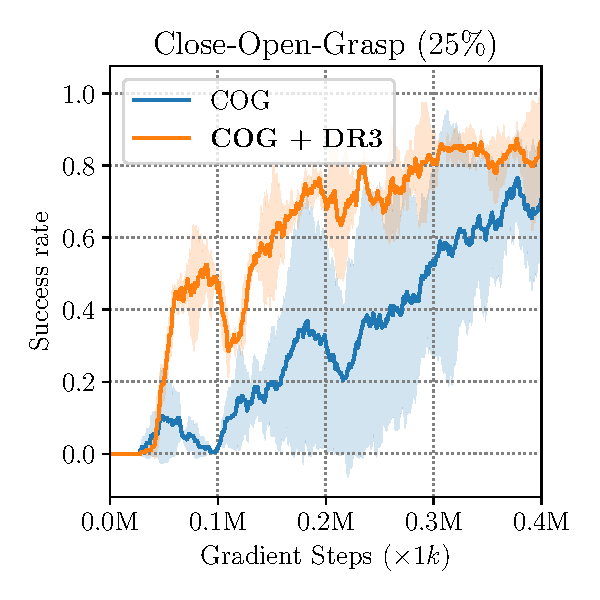
\includegraphics[width=0.49\linewidth]{figures/Widow250DoubleDrawerCloseOpenGraspNeutral-v0_cog_vs_dr3_25_v2.pdf}
% % 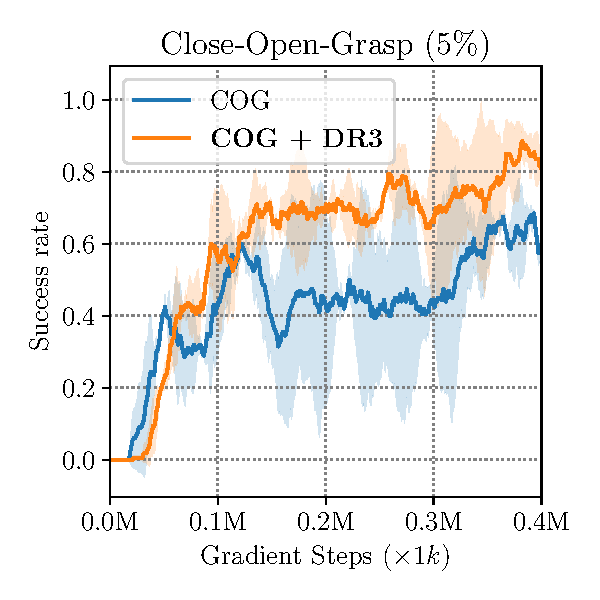
\includegraphics[width=0.49\linewidth]{figures/Widow250DoubleDrawerCloseOpenGraspNeutral-v0_cog_vs_dr3_25_v3.pdf}
% % 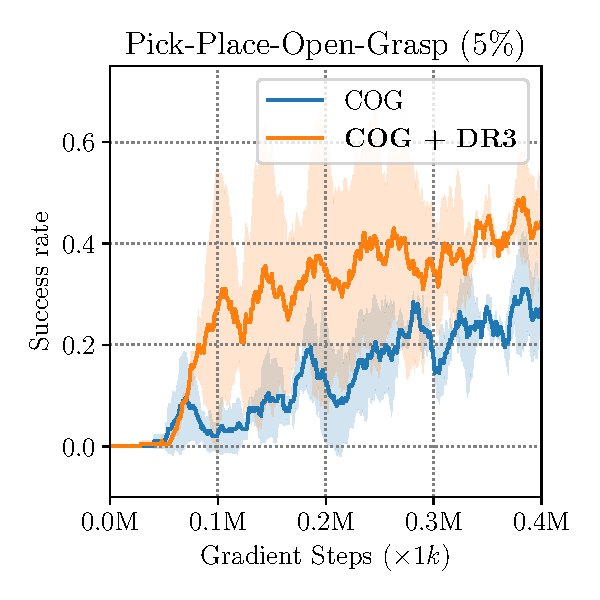
\includegraphics[width=0.49\linewidth]{figures/Widow250DoubleDrawerPickPlaceOpenGraspNeutral-v0_cog_vs_dr3_25_v4.pdf}
% % 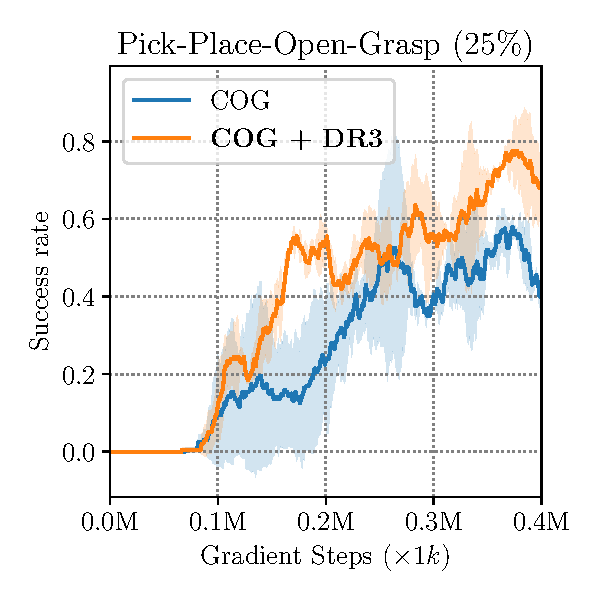
\includegraphics[width=0.49\linewidth]{figures/Widow250DoubleDrawerPickPlaceOpenGraspNeutral-v0_cog_vs_dr3_25.pdf}
% 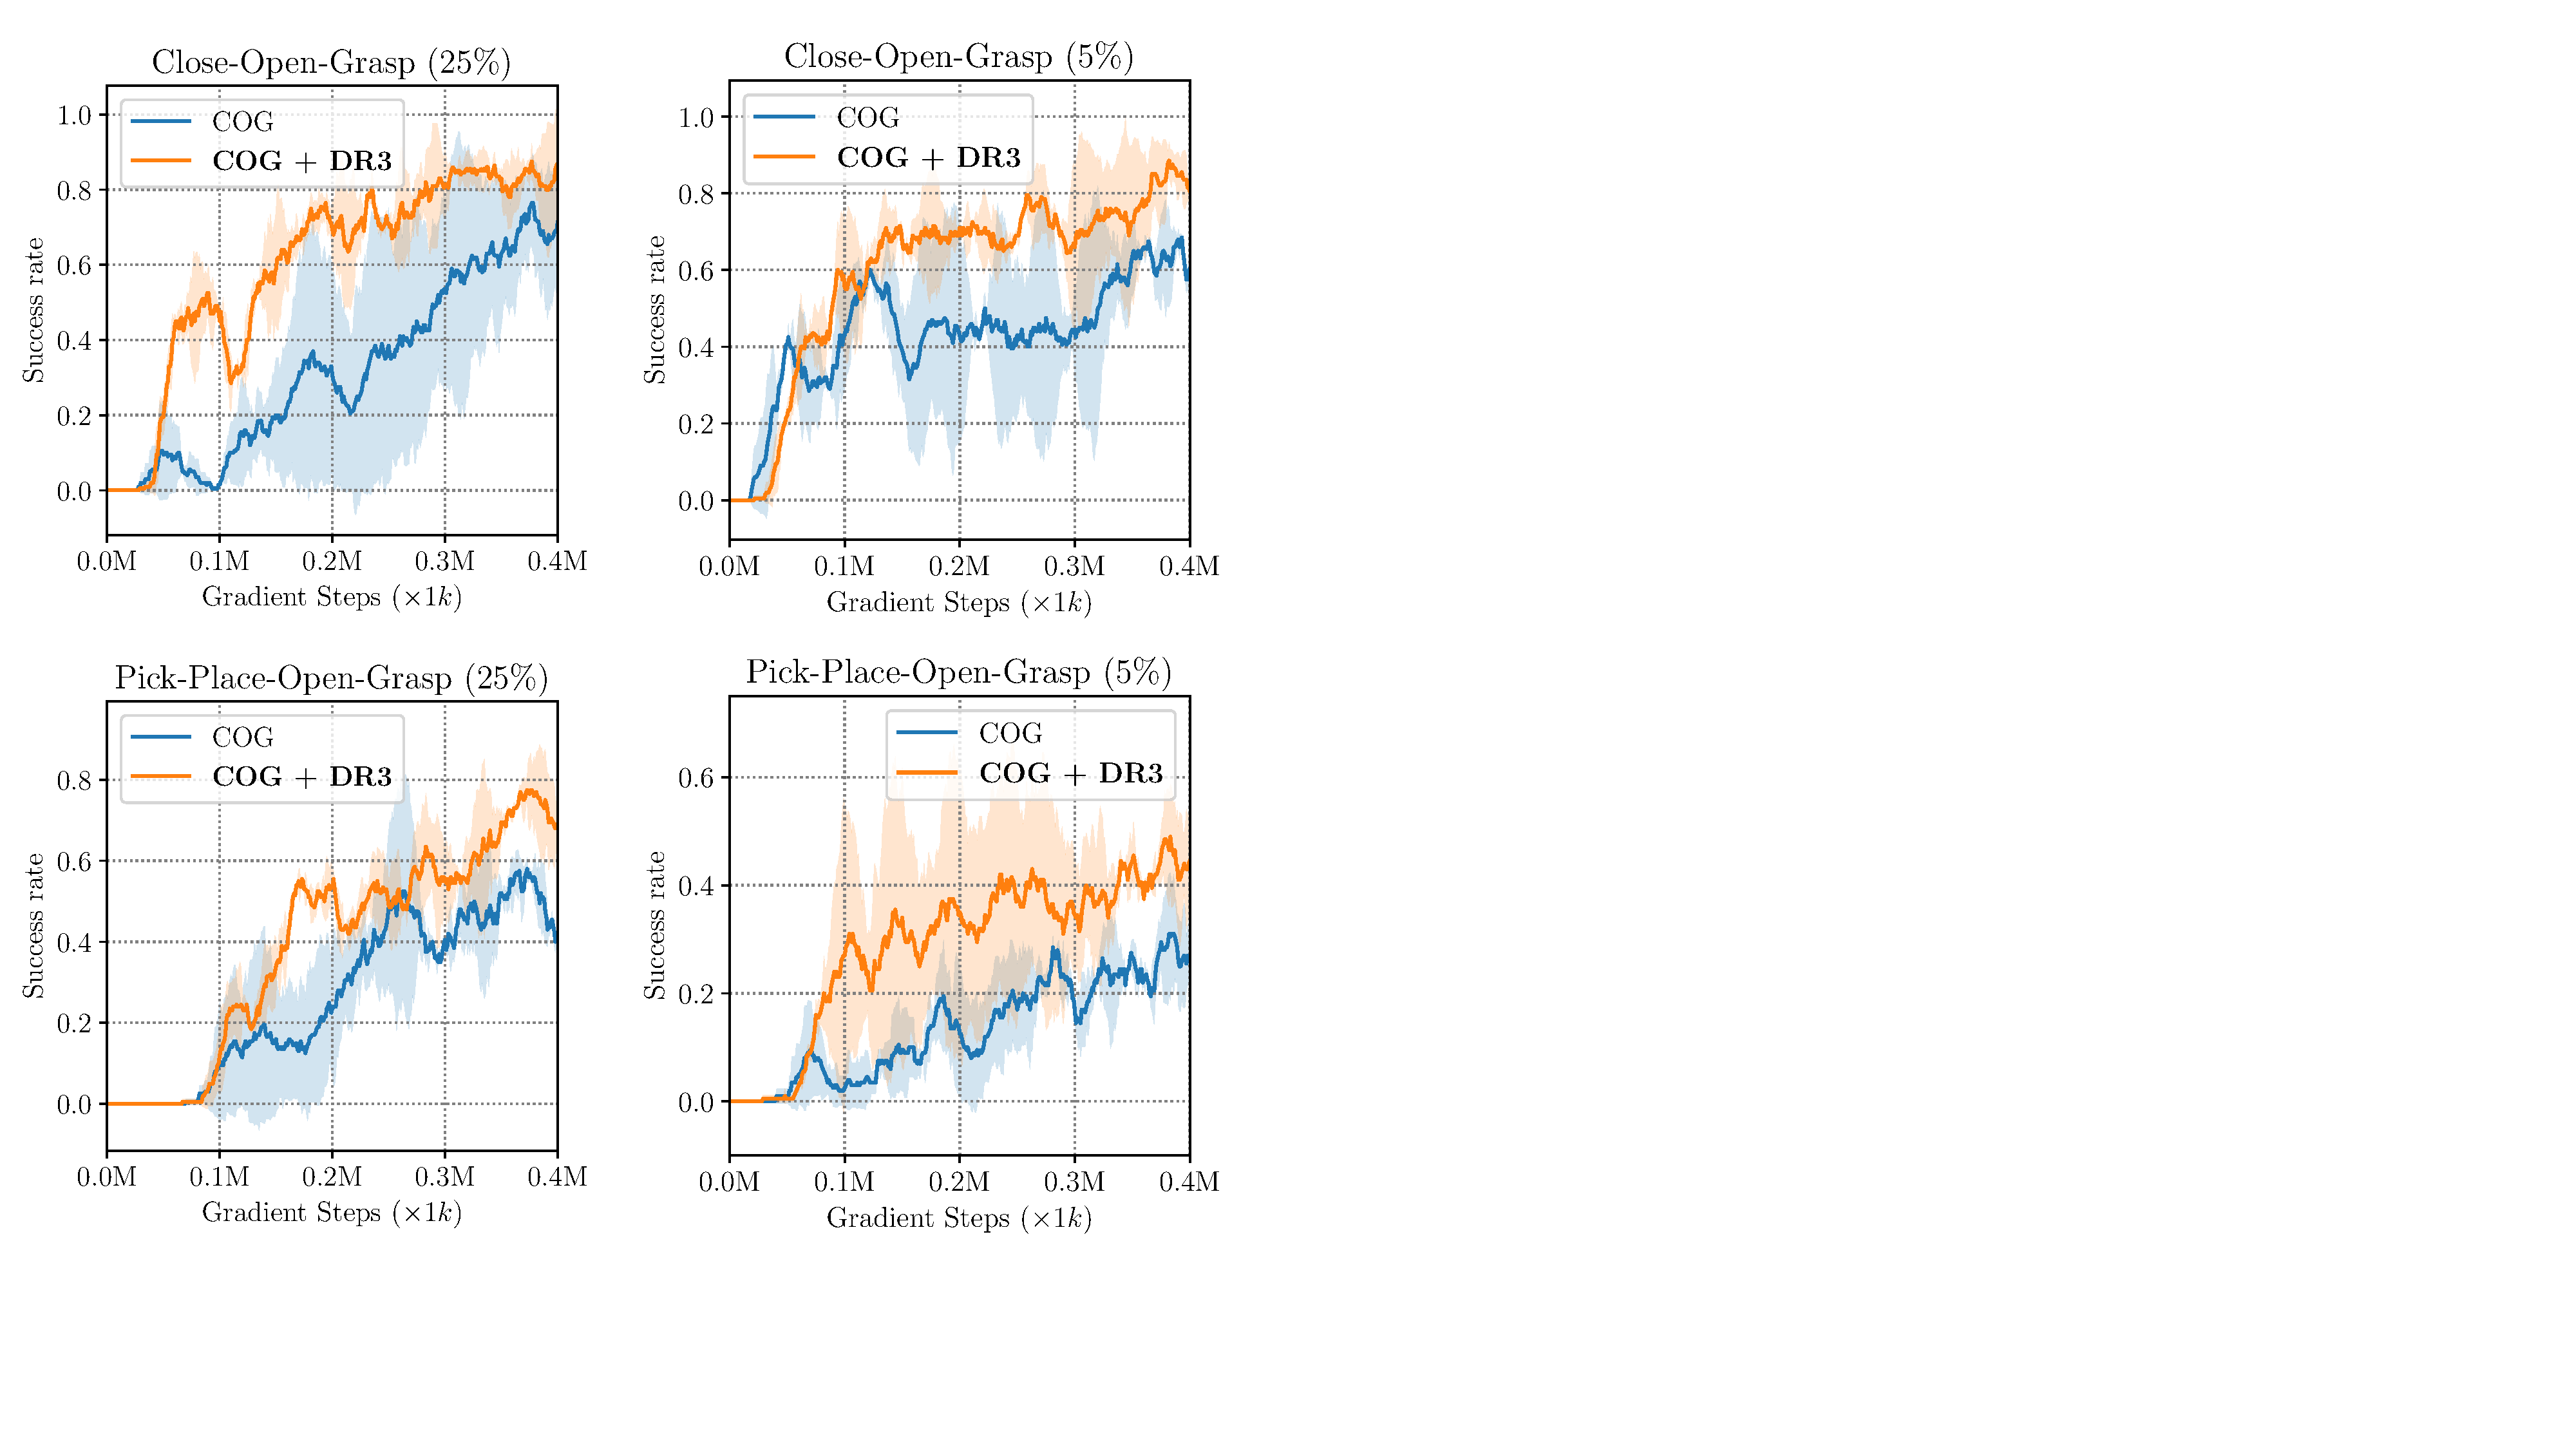
\includegraphics[width=0.5\linewidth]{figures/cog_plots.pdf}
% \end{center}
% \vspace{-15pt}
% \caption{\small{\textbf{Performance of \methodname\ + COG} on four robotic manipulation settings with different amounts of data. As is visible, COG + \methodname\ always outperforms COG and attains higher average and final performance.}}
% \vspace{-5pt}
% \label{fig:cog_figure}
% \end{figure}


%%%%%%%%%%%%%%%%%%%%%%%%% OLD TABLE %%%%%%%%%%%%%%%%%%%%%%%%%%%%%%%
% \begin{figure*}
% % \hline
%     \begin{minipage}{.5\textwidth}
%     \centering
%     \vspace{-0.01in}
%     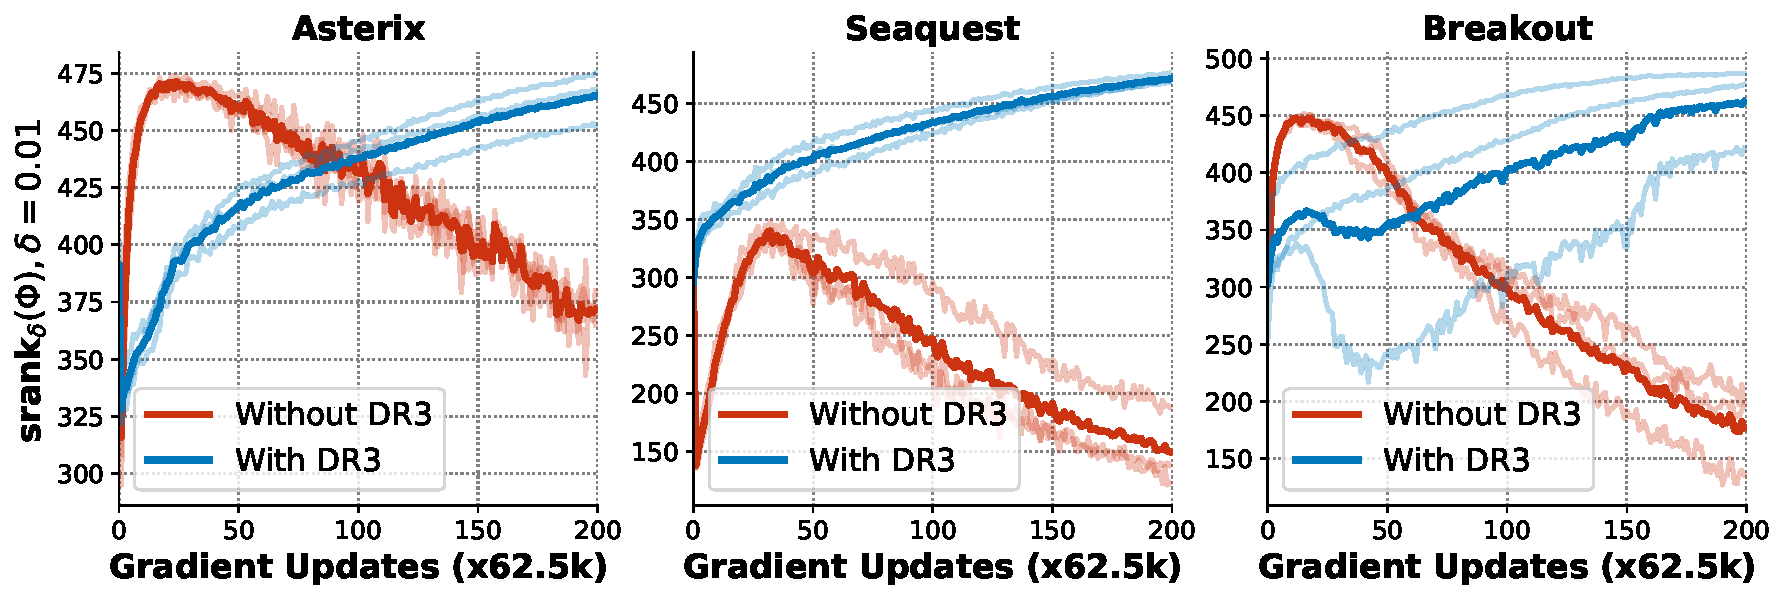
\includegraphics[width=0.99\linewidth]{figures/rank_trends_dr3_dqn.pdf}
%     % 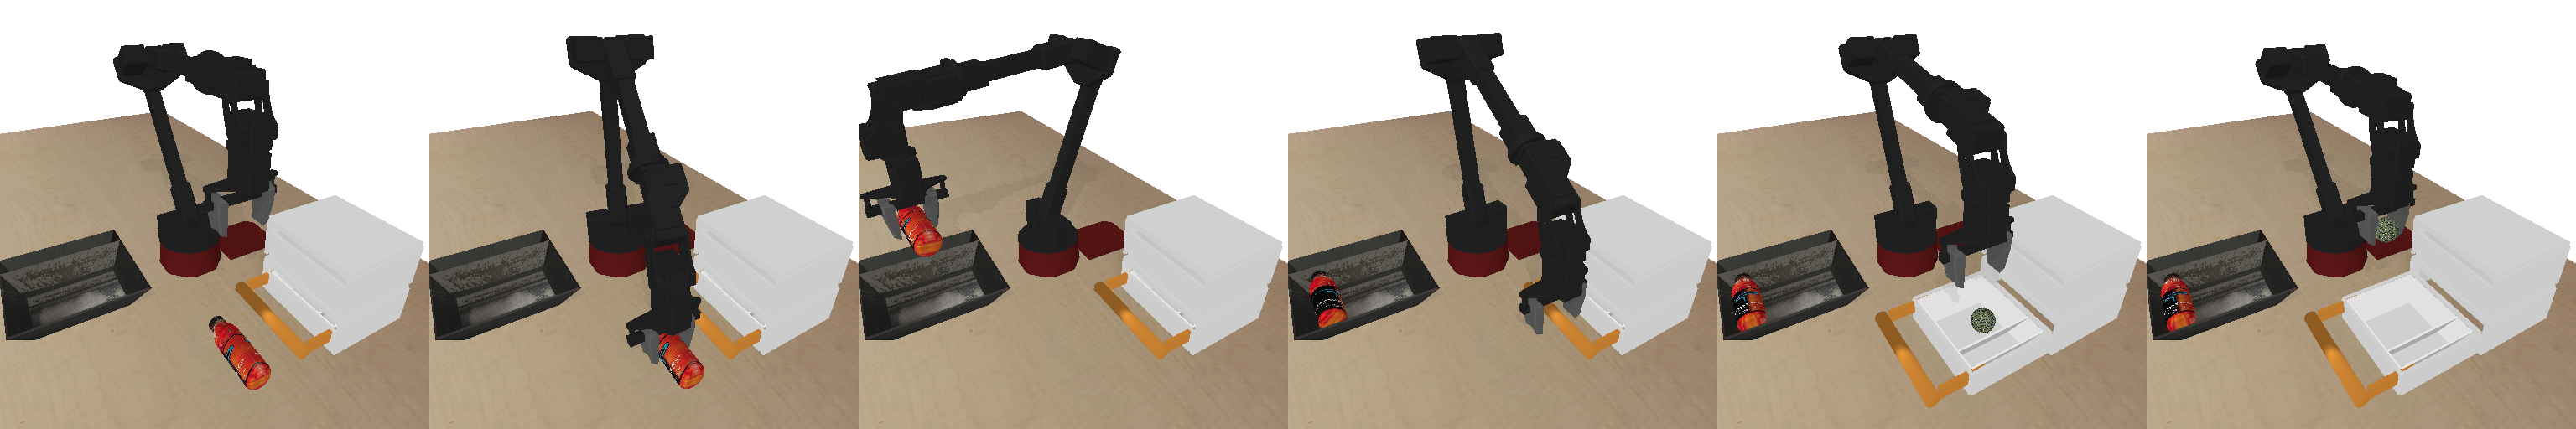
\includegraphics[width=\linewidth]{figures/pickplace_open_grasp.png}
%     \vspace{-0.2in}
%     \caption{\footnotesize{{\textbf{Trend of effective rank,} $\mathrm{srank}(\Phi)$ of features $\Phi$ learned by the Q-function when trained with TD error (red, ``Without DR3'') and with TD error + \methodname\ (blue, ``With DR3'') on three Atari games using the 5\% dataset. Note that \methodname\ alleviates rank collapse observed by \citet{kumar2021implicit}, without explicitly aiming to. Effective rank measures the number of directions with significant singular values~(Appendix~\ref{app:rank_collapse_is_gone}).}}}
%     \label{fig:iup_is_fixed}
%     \vspace{-0.25in}
%     \end{minipage}~~\vline~~
%     \begin{minipage}{.47\textwidth}
%     % \begin{table}[t]
%     % % \vspace{-0.8cm}
%     \vspace{-0.05in}
%     \fontsize{8}{8}\selectfont
%     \centering
%     \captionof{table}{\footnotesize{\textbf{Performance of CQL, CQL + \methodname\ after 2M gradient steps with a learning rate of 3e-4} for the Q-function averaged over 4 seeds. This is training for \textbf{6x} longer compared to CQL defaults. Observe that CQL + \methodname\ outperforms CQL at 2M steps, indicating is efficacy in inducing stability. %``\texttt{med}'' stands for medium and ``\texttt{lar}'' stands for large.
%     }}
%     \label{tab:cql_d4rl}
%     \vspace{-0.1in}
%     \begin{tabular}{@{}lrr@{}}
%     \toprule
%     {\textbf{D4RL (-v0) Task}} & CQL & CQL + \methodname \\
%     \midrule
%     \texttt{kitchen-mixed} & 14.6 $\pm$ 20.5 & \textbf{37.0 $\pm$ 8.0} \\
%     \texttt{kitchen-partial} & 29.6 $\pm$ 19.6 & \textbf{43.5 $\pm$ 1.9}  \\
%     \texttt{kitchen-complete} & 22.3 $\pm$ 17.5 & 24.8 $\pm$ 15.3 \\
%     \midrule
%     \texttt{antmaze-med-diverse} & 0.7 $\pm$ 0.1 & \textbf{0.9 $\pm$ 0.1} \\
%     \texttt{antmaze-med-play} & 0.5 $\pm$ 0.4 & 0.4 $\pm$ 0.3 \\
%     \texttt{antmaze-lar-diverse} & 0.1 $\pm$ 0.0 & \textbf{0.3 $\pm$ 0.16}\\
%     \texttt{antmaze-lar-play} & 0.06 $\pm$ 0.09 & 0.1 $\pm$ 0.01 \\
%     \bottomrule
%     \end{tabular}
%     \vspace{-0.5cm}
%     \end{minipage}
% \end{figure*}
% \hline
% \begin{table}[t]
% % \vspace{-0.8cm}
% \fontsize{8}{8}
% \centering
% \caption{\small{Performance of CQL, CQL + \methodname\ after 2M (twice as long as prior work) gradient steps with a learning rate of 3e-4 for the Q-function averaged over 4 seeds. We also find that CQL + \methodname\ outperforms CQL at 2M steps, and is comparable to CQL when evaluated at 1M steps, which was the protocol followed originally. ``\texttt{med}'' stands for medium and ``\texttt{lar}'' stands for large.}}
% \label{tab:cql_d4rl}
% \small{
% % \vspace{0.2cm}
% \begin{tabular}{l||r|r}
% \toprule
% {\textbf{D4RL (-v0) Task}} & CQL & \textbf{CQL + \methodname} \\
% \midrule
% \texttt{kitchen-mixed} & 14.58 $\pm$ 20.49 & \textbf{37.04 $\pm$ 8.04} \\
% \texttt{kitchen-partial} & 29.63 $\pm$ 19.58 & \textbf{43.54 $\pm$ 1.90}  \\
% \texttt{kitchen-complete} & 22.27 $\pm$ 17.51 & 24.77 $\pm$ 15.3 \\
% \midrule
% \texttt{antmaze-med-diverse} & 0.73 $\pm$ 0.12 & \textbf{0.90 $\pm$ 0.08} \\
% \texttt{antmaze-med-play} & 0.47 $\pm$ 0.36 & 0.36 $\pm$ 0.26 \\
% \texttt{antmaze-lar-diverse} & 0.10 $\pm$ 0.00 & \textbf{0.27 $\pm$ 0.16}\\
% \texttt{antmaze-lar-play} & 0.06 $\pm$ 0.09 & \textbf{0.1 $\pm$ 0.01} \\
% \bottomrule
% \end{tabular}}
% \vspace{-0.5cm}
% \end{table}
%%%%%%%%%%%%%%%%%%%%%%%%%%%%%%%%%%%%%%%%%%%%%%%%%%%%%%%%%%%%%%%%%%%%%%%%%%%%%%%%

% \textbf{{Offline RL on D4RL tasks.}} Finally, we evaluate DR3 in conjunction with CQL on the antmaze and kitchen domains in D4RL~\citep{fu2020d4rl}. To assess if \methodname\ is stable and able to prevent unlearning that eventually appears in CQL, we trained CQL+\methodname\ for \textbf{6x} longer: 2M steps with 3x higher learning rate. %This is different from prior works~\citep{kumar2020conservative} that report performance at the end of 1M steps.
% Observe in Table~\ref{tab:cql_d4rl}, that CQL + \methodname\ outperforms CQL ({statistical significance shown in Appendix~\ref{app:significance}}). {We show that CQL + DR3 also outperforms base CQL in terms of performance and stability on MuJoCo tasks previously studied in \citet{kumar2021implicit} in Appendix~\ref{app:mujoco}.} 
% %%SL.10.2: I don't see how "indicating the ability to train for more gradient steps" follows from these results -- where is the evidence for this? did you change the number of steps? Also, this section appears to violate what you said before about reporting stability: you said that stability = average over iterations, but here you are not reporting it. If this is how it is, then maybe revise the beginning of the experiments section, which makes a really big deal out of this stability metric. I *think* what you mean is that training for 2M steps evaluates stability better than 1M steps, but critical readers will just say you cherry-picked the number of steps that makes your method look good.
% Further, we also compare the effect of adding \methodname\ to BRAC~\citep{wu2019behavior}.
% %%SL.10.2: such as BRAC, or just BRAC?
% \methodname\ applied on BRAC improves final median normalized score performance by \textbf{13.8}  and stability by \textbf{8.1} across 15 MuJoCo tasks. Numbers for BRAC can be found in Table~\ref{tab:brac}.
% %%AK: unfortunately this table is in the Appendix.

\textbf{{Offline RL on D4RL tasks.}} Finally, we evaluate DR3 in conjunction with CQL on the antmaze-v2 domain in D4RL~\citep{fu2020d4rl}. To assess if \methodname\ is stable and able to prevent unlearning that eventually appears in CQL, we trained CQL+\methodname\ for \textbf{9x} longer: 2M and 3M steps with 3x higher learning rate. This is different from prior works~\citep{fu2020d4rl} that report performance at the end of 1M steps.
Observe in Table~\ref{tab:cql_d4rl}, that CQL + \methodname\ outperforms CQL ({statistical significance shown in Appendix~\ref{app:significance}}), indicating that DR3 significantly improves CQL. We also evalute DR3 on kitchen domains in D4RL in Appendix~\ref{app:significance}, where we also find that DR3 improves CQL. Finally, we also compare CQL+DR3 and CQL in terms of performance and stability on MuJoCo tasks previously studied in \citet{kumar2021implicit} in Appendix~\ref{app:mujoco}. These tasks are constructed by uniformly subsampling transitions from the full-replay-v2 MuJoCo datasets in D4RL and are much harder than the typical Gym-MuJoCo tasks from \citet{fu2020d4rl} because succeeding on these tasks critically relies on estimating accurate Q-values for out-of-sample actions and all actions at certain states are out-of-sample. As shown in Appendix~\ref{app:mujoco}, CQL+DR3 is significantly more stable, and does not unlearn with more training, unlike CQL whose performance degrades very quickly. We also evaluate DR3 in conjunction with BRAC~\citep{wu2019behavior}, a policy constraint method, and find that BRAC+DR3 improves over BRAC in \textbf{13.8} median normalized performance (Table~\ref{tab:brac}).
% \textbf{These results} indicate that \methodname\ is a versatile explicit regularizer that improves performance and stability of a wide range of offline RL methods. 

\begin{table*}[t]
    % \begin{table}[t]
    % % \vspace{-0.8cm}
    % \vspace{-0.25cm}
    \fontsize{8}{8}\selectfont
    \centering
    \captionof{table}{\footnotesize{\textbf{Performance of CQL, CQL + \methodname\ after 2M and 3M gradient steps with a learning rate of 3e-4} for the Q-function averaged over 3 seeds. This is training for \textbf{6x} and \textbf{9x} longer compared to CQL defaults. Observe that CQL + \methodname\ outperforms CQL at 2M and 3M steps, indicating is efficacy in preventing unlearning. We present the statistical significance of these results in Appendix~\ref{app:significance}.}}
    \label{tab:cql_d4rl}
    \vspace{-0.1in}
    \begin{tabular}{@{}l|rr||rr@{}}
    \toprule
    {\textbf{D4RL Task}} & \textbf{CQL} (2M) & \textbf{CQL + \methodname} (2M) & \textbf{CQL} (3M) & \textbf{CQL + \methodname} (3M)  \\
    \midrule
    % \texttt{kitchen-mixed} & 14.6 $\pm$ 20.5 & \textbf{37.0 $\pm$ 8.0} \\
    % \texttt{kitchen-partial} & 29.6 $\pm$ 19.6 & \textbf{43.5 $\pm$ 1.9}  \\
    % \texttt{kitchen-complete} & 22.3 $\pm$ 17.5 & 24.8 $\pm$ 15.3 \\
    % \midrule
    \texttt{antmaze-umaze-v2} & 84.00 $\pm$ 2.67 & 85.33 $\pm$ 4.16 & 87.00 $\pm$ 1.73 & 90.00 $\pm$ 4.00 \\ 
    \texttt{antmaze-umaze-diverse-v2} & 45.67 $\pm$ 8.50 & 40.67 $\pm$ 11.84 & 36.33 $\pm$ 7.09 & \textbf{52.00 $\pm$ 11.26} \\
    \texttt{antmaze-medium-play-v2} & 24.00 $\pm$ 28.16 & \textbf{73.00 $\pm$ 4.00} & 16.00 $\pm$ 26.85 & \textbf{71.33 $\pm$ 1.52} \\
    \texttt{antmaze-medium-diverse-v2} & 32.67 $\pm$ 9.29 & \textbf{67.00 $\pm$ 2.00} & 48.33 $\pm$ 6.11 & \textbf{61.67 $\pm$ 3.21} \\
    \texttt{antmaze-large-play-v2} & 3.33 $\pm$ 2.51 & \textbf{28.00 $\pm$ 4.35} & 0.33 $\pm$ 0.57 & \textbf{26.33 $\pm$ 11.93} \\
    \texttt{antmaze-large-diverse-v2} & 1.33 $\pm$ 2.30 & \textbf{25.67 $\pm$ 0.57} & 0.00 $\pm$ 0.00 & \textbf{28.33 $\pm$ 1.52} \\
    \bottomrule
    \end{tabular}
    \vspace{-0.4cm}
    \end{table*}



% \begin{wrapfigure}{r}{0.57\textwidth}
% \small \begin{center}
% \vspace{-0.3in}
% 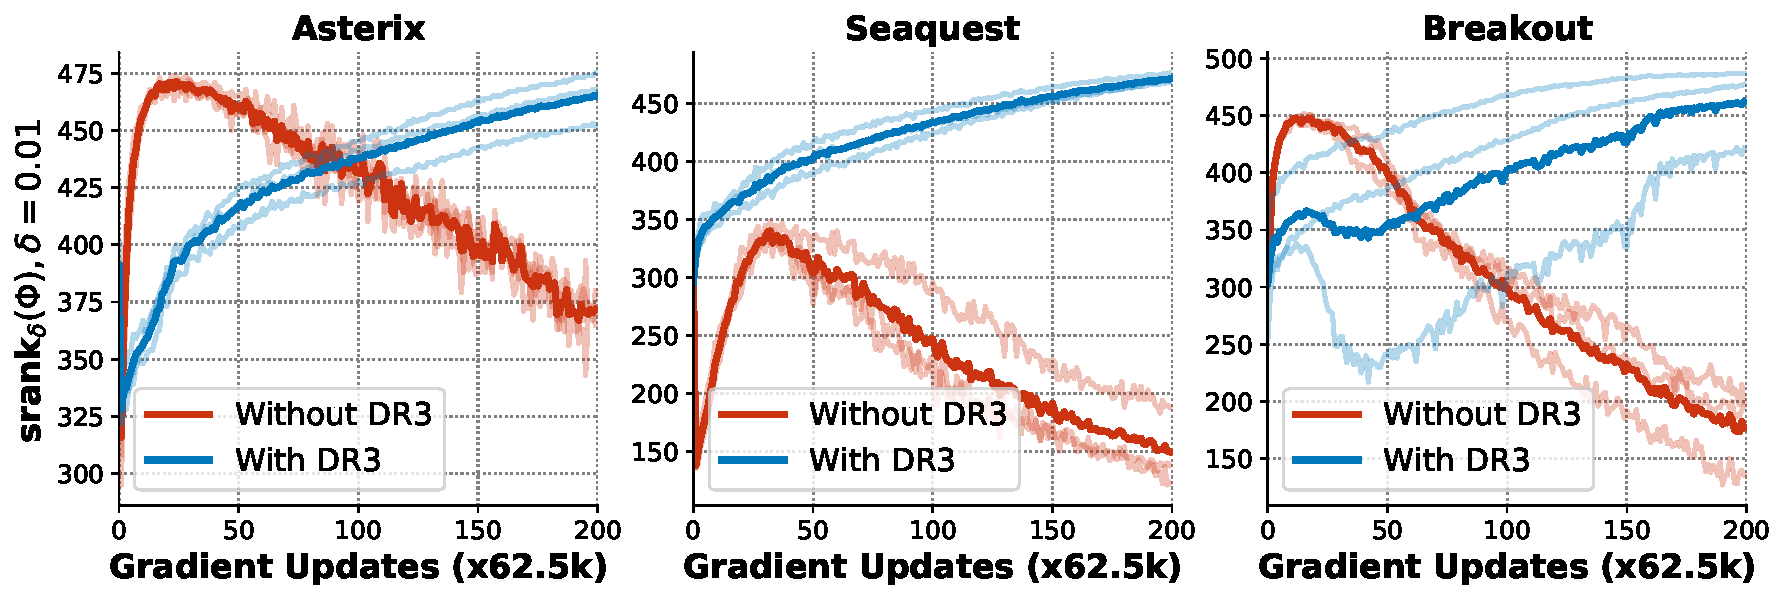
\includegraphics[width=0.99\linewidth]{figures/rank_trends_dr3_dqn.pdf}
% % 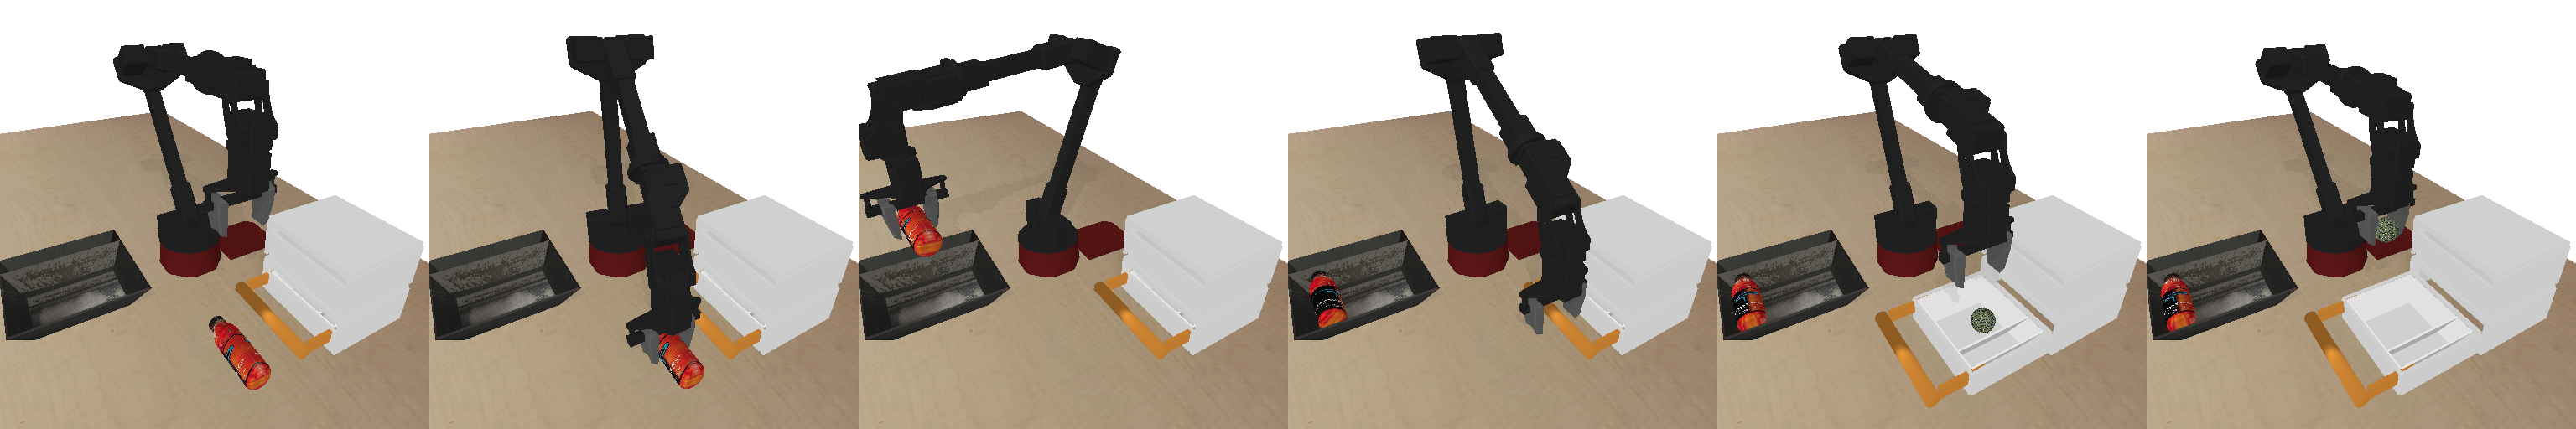
\includegraphics[width=\linewidth]{figures/pickplace_open_grasp.png}
% \vspace{-0.1in}
% \caption{\small{{\textbf{Trend of effective rank,} $\mathrm{srank}(\Phi)$ of features $\Phi$ learned by the Q-function when trained with TD error (red, ``Without DR3'') and with TD error + \methodname\ (blue, ``With DR3'') on three Atari games using the 5\% dataset. Note that \methodname\ clearly alleviates rank collapse, without explicitly aiming to.}}}
% \label{fig:iup_is_fixed}
% \end{center}
% \vspace{-0.25in}
% \end{wrapfigure}
\begin{figure}[h]
    \centering
    \vspace{-0.1in}
    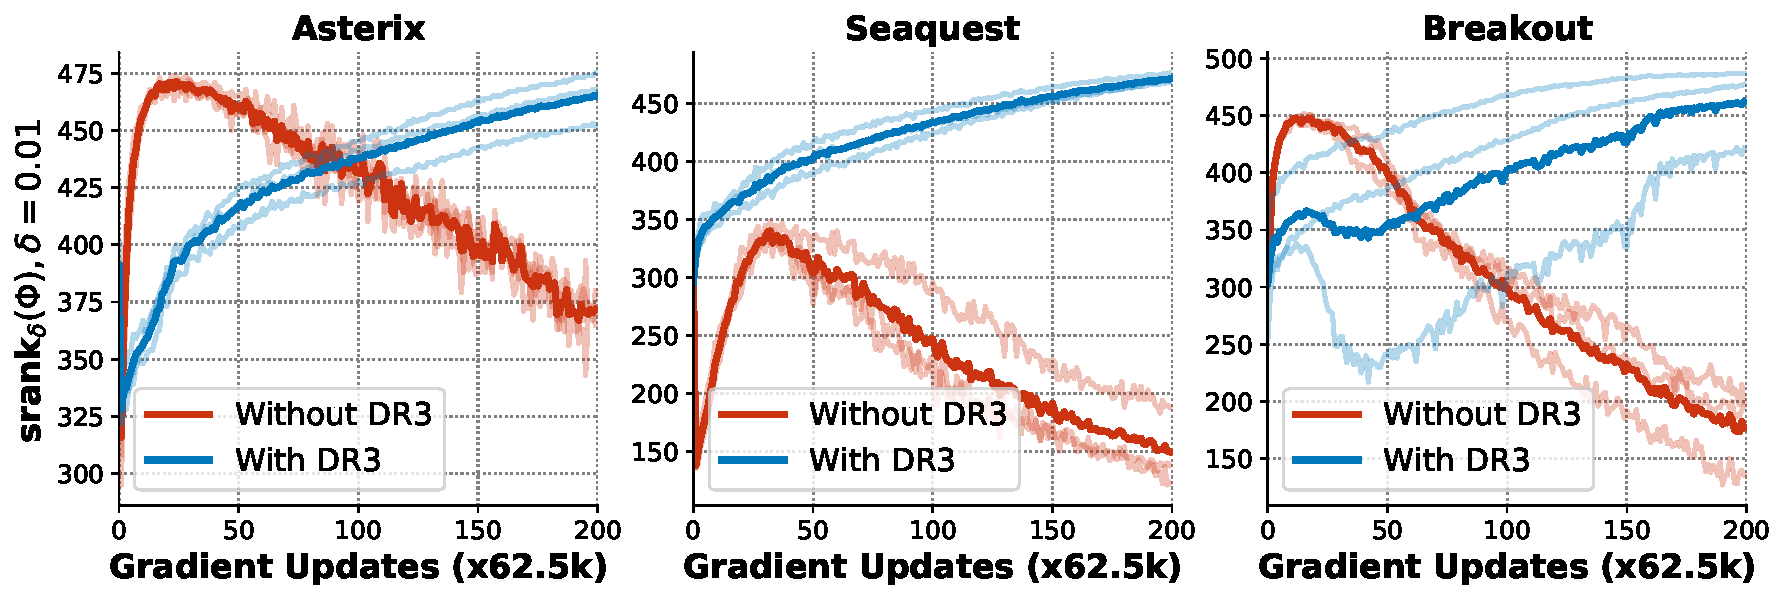
\includegraphics[width=0.8\linewidth]{figures/rank_trends_dr3_dqn.pdf}
    % 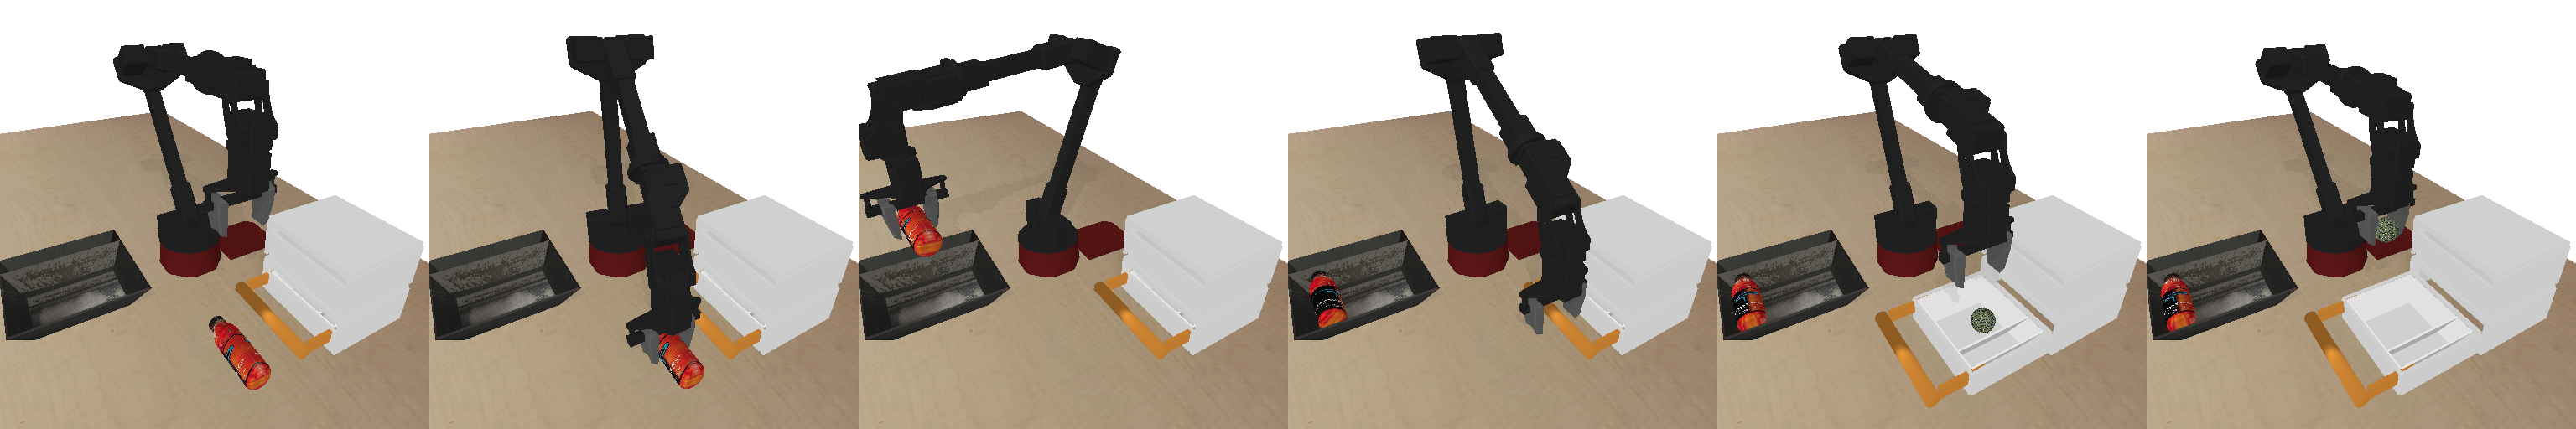
\includegraphics[width=\linewidth]{figures/pickplace_open_grasp.png}
    \vspace{-0.1in}
    \caption{\footnotesize{{\textbf{Trend of effective rank,} $\mathrm{srank}(\Phi)$ of features $\Phi$ learned by the Q-function when trained with TD error (red, ``Without DR3'') and with TD error + \methodname\ (blue, ``With DR3'') on three Atari games using the 5\% dataset. Note that \methodname\ alleviates rank collapse, without explicitly aiming to.}}}
    \label{fig:iup_is_fixed}
    \vspace{-0.1in}
\end{figure}
\textbf{{{DR3 does not suffer from rank collapse.}}} Prior work~\citep{kumar2021implicit} has shown that implicit regularization can lead to a rank collapse issue in TD-learning, preventing Q-networks from using full capacity. To see if \methodname\ addresses the rank collapse issue, we follow \citet{kumar2021implicit} and plot the effective rank of learned features with DR3 in Figure~\ref{fig:iup_is_fixed} {(DQN, REM in Appendix~\ref{app:rank_collapse_is_gone})}. 
%%AK: removed definition in the interest of space
% Effective rank of a matrix $\bM \in  \mathbb{R}^{n \times d}, n > d$ for a given threshold $\delta$ is given by: $\mathrm{srank}_\delta(\bM) = \min \{k: \frac{\sum_{i=1}^k \sigma_i(\bM)}{\sum_{i=1}^d \sigma_i(\bM)} \geq 1 - \delta \}$, where $\{\sigma_i(\bM)\}$ denotes the singular values of $\bM$ arranged in decreasing order. 
While the value of the effective rank decreases during training with na\"ive bootstrapping, {we find that rank of DR3 features typically does not collapse}, despite no explicit term encouraging this. 
% as shown in Figure~\ref{fig:iup_is_fixed}.  
Finally, we test the robustness/sensitivity of each layer in the learned Q-network to re-initialization~\citep{zhang2019all} during training and find that DR3 alters the features to behave similarly to supervised learning~(\Figref{fig:robustness}).

%%AK: This discussion is a bit redundant with what is there in the technical section already, so I can just move it there.
\begin{figure}[t]
\small \begin{center}
\vspace{-0.2cm}
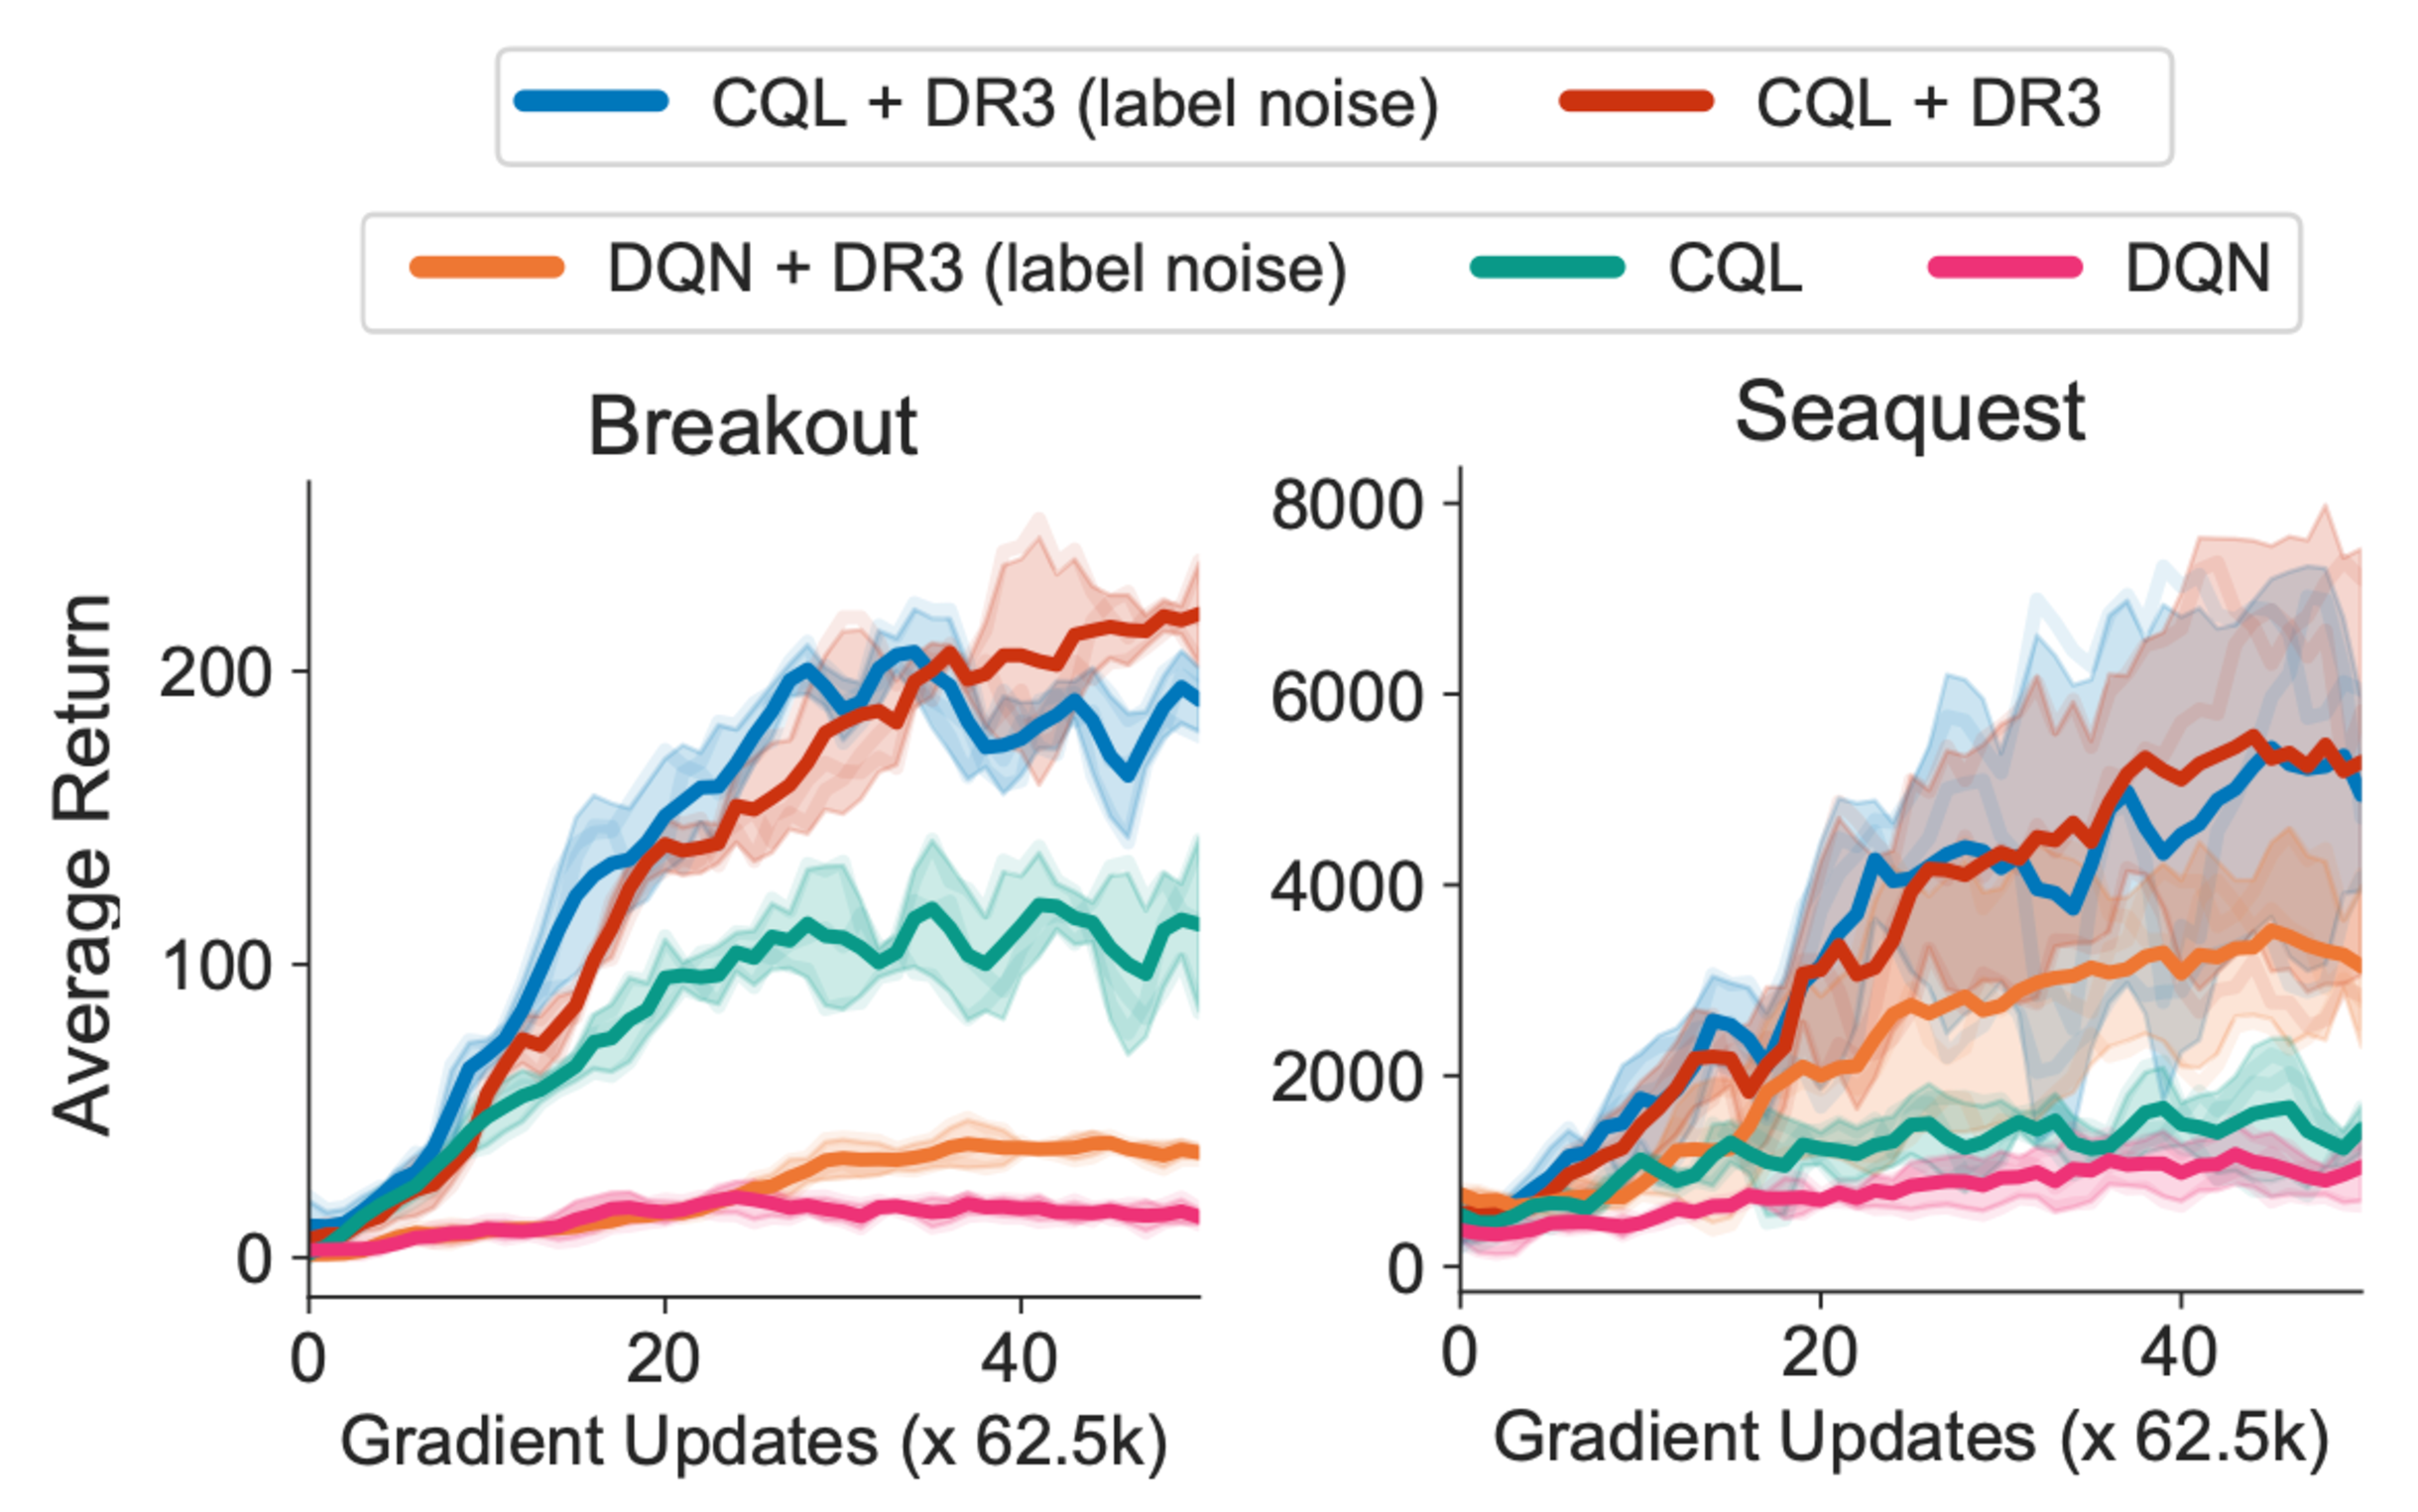
\includegraphics[width=0.6\linewidth]{figures_iclr/different_penalty.pdf}
\vspace{-10pt}
\caption{\label{fig:other_penalty_main} \footnotesize{Comparing  DR3 for our simplifying choice of $M$, and $M$ induced by label noise, {with base CQL and DQN algorithms}. Note that both of these penalties when applied over CQL improve performance.}}
\end{center}
\vspace{-0.2in}
\end{figure}
\textbf{Comparing explicit regularizers for different choices of noise covariance $M$.} Finally, we investigate the behavior of different implicit regularizers derived via two choices of $M$ in Equation~\ref{eqn:regularizer} and the corresponding explicit regularizers. While the explicit regularizer we use in practice is a simplifying choice that works well, another choice of $M$ is the covariance matrix induced by label noise, which requires explicit computation of $\Sigma_M^*$.
%%SL.10.2: This is very important. But I also don't like the weasel words here. We are trying to say that \Sigma_M = I is just another "choice". But critical readers will see right through this. It's not another choice, it's a hack to make it easy to implement, and we should just admit this. It's OK to present an interpretation of it as just another choice for M too, but we should definitely not attempt to hide that it's a hack. Just admit it's a hack, and say we use it because it works well, otherwise reviewers will believe the paper is being deceptive.
Observe in Figure~\ref{fig:other_penalty_main} that the {explicit regularizer for our simplifying choice is not worse than the different choice of $M$}. This justifies utilizing our simplified, heuristic choice of setting $\Sigma_M^* = I$ in practice. Results on five Atari games are shown in Appendix~\ref{app:theory_practice_gap}.       
% Since \methodname\ is directly derived as a way to mitigate the undesirable effect of implicit regularization of the TD update, utilizing it directly address the rank collapse issue as compared to a penalty artificially created to tackle ths phenomenon.
% \textbf{Data-Efficient online RL.} Finally, we evaluate the performance of \methodname\ on ``data-efficient'' online RL tasks from the Atari-100K benchmark~\citep{kaiser2019model,van2019use}, where the goal is learn a peformant policy as quickly as possible. On these tasks, we apply \methodname\ on data-efficient rainbow (DER)~\citep{van2018deep}, and compare the final performance at 100k environment steps.
%%AK: we need to also measure equivalent of average?


% \begin{table}[h]
% \fontsize{8}{8}
% \centering
% \caption{Performance of \methodname\ when applied in conjunction with BRAC~\citep{wu2019behavior}. Note that DR3 attains a larger final performance (at the end of 2M steps of training) as well as a higher average performance (i.e. stability score) across all iterations of training.}
% \label{tab:brac}
% \vspace{0.2cm}
% \begin{tabular}{ccccc}
% \toprule
% \multirow{2}{*}{Task} & \multicolumn{2}{c}{Average Performance}   & \multicolumn{2}{c}{Final Performance} \\
% & BRAC & BRAC + \methodname & BRAC & BRAC + \methodname \\
% \midrule
% %('True', '0.1', '2')
% halfcheetah-exp & 1.7 $\pm$ 1.9 & 49.9 $\pm$ 16.7  & 2.1 $\pm$ 3.3 & 71.5 $\pm$ 24.9 \\
% halfcheetah-med & 43.5 $\pm$ 0.2 & 43.2 $\pm$ 0.2  & 45.1 $\pm$ 0.8 & 44.9 $\pm$ 0.6 \\
% halfcheetah-med-exp & 17.0 $\pm$ 5.4 & 6.0 $\pm$ 5.5  & 24.8 $\pm$ 9.3 & 6.7 $\pm$ 7.3 \\
% halfcheetah-rand & 24.4 $\pm$ 0.4 & 18.4 $\pm$ 0.3  & 24.9 $\pm$ 0.8 & 18.2 $\pm$ 1.0 \\
% % halfcheetah-med-replay & 44.9 $\pm$ 0.3 & 44.1 $\pm$ 0.4  & 45.0 $\pm$ 1.4 & 44.9 $\pm$ 0.5 \\
% hopper-exp & 15.7 $\pm$ 1.5 & 21.8 $\pm$ 3.2  & 16.6 $\pm$ 6.0 & 20.8 $\pm$ 5.3 \\
% hopper-med & 32.8 $\pm$ 1.4 & 46.3 $\pm$ 7.1  & 36.2 $\pm$ 1.7 & 58.3 $\pm$ 13.7 \\
% hopper-med-exp & 40.2 $\pm$ 5.7 & 37.0 $\pm$ 2.9  & 31.7 $\pm$ 11.8 & 21.8 $\pm$ 4.9 \\
% hopper-rand-v0 & 11.7 $\pm$ 0.0 & 11.2 $\pm$ 0.0  & 12.2 $\pm$ 0.0 & 11.1 $\pm$ 0.0 \\
% hopper-med-replay & 31.6 $\pm$ 0.3 & 30.3 $\pm$ 0.8  & 31.3 $\pm$ 1.2 & 36.1 $\pm$ 5.7 \\
% walker2d-exp & 25.5 $\pm$ 14.4 & 33.6 $\pm$ 11.8  & 54.0 $\pm$ 31.0 & 60.6 $\pm$ 20.2 \\
% walker2d-med & 81.3 $\pm$ 0.3 & 80.8 $\pm$ 0.2  & 83.8 $\pm$ 0.2 & 83.4 $\pm$ 0.3 \\
% walker2d-med-exp & 5.8 $\pm$ 5.2 & 6.4 $\pm$ 3.4  & 22.4 $\pm$ 22.0 & 39.5 $\pm$ 23.3 \\
% walker2d-rand & 1.4 $\pm$ 0.8 & 1.7 $\pm$ 0.9  & 0.0 $\pm$ 0.1 & 2.9 $\pm$ 2.1 \\
% walker2d-med-replay & 26.1 $\pm$ 6.4 & 47.4 $\pm$ 4.1  & 11.7 $\pm$ 7.0 & 38.7 $\pm$ 9.6 \\
% \midrule
% Median Normalized Perf. & 25.5 & \textbf{33.6} & 24.9 & \textbf{38.7} \\
% Mean Normalized Perf. & 26.9 & \textbf{31.9} & 29.5 & \textbf{37.3} \\
% \bottomrule
% \end{tabular}
% \end{table}









% \subsection{Offline Policy Evaluation}
% d4rl, cite DOPE benchmark, FQE is best already
% comparable on most tasks, and improvements on a few tasks. Antmaze and mujoco similar.
% \begin{figure*}[t]
%     \centering
%     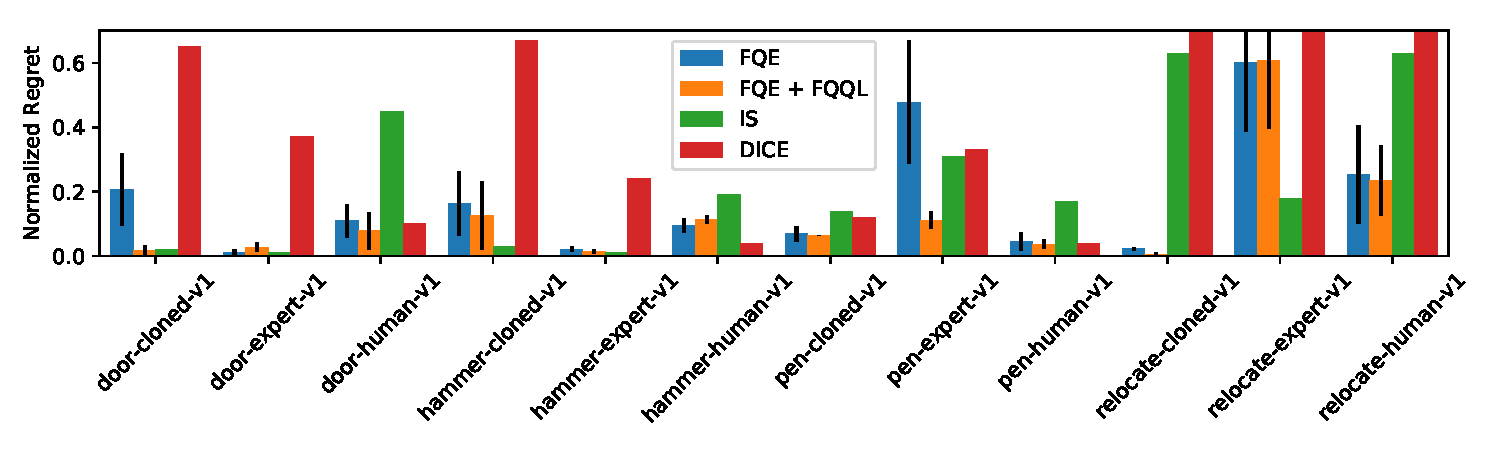
\includegraphics[width=\linewidth]{figures/Normalized Regret.pdf}
%     \vspace{-0.65cm}
%     \caption{Normalized regret on harder benchmark offline policy evaluations tasks in the DOPE benchmark~\citep{fu2021benchmarks}. Lower regret is better. We report the mean over 5 seeds and SEM. We use the benchmark numbers for IS and DICE from~\citep{fu2021benchmarks}.}
%     \label{fig:fqe}
% \end{figure*}

% \vspace{-8pt}
% \section{Experimental Evaluation of \methodname}
% \label{sec:experiments}
% \vspace{-8pt}
% % The goal of our experiments is to verify the claim that value-based deep RL methods require explicit regularization, as well as to evaluate the efficacy of our practical approach, \methodname, in addressing regularization challenges.
% %%SL.10.2: I wonder if some readers might question whether our experiments really verify that it *requires* explicit regularization. We could say rather it aims to understand whether feature co-adaptation is a major issue empirically or something. But it actually doesn't look like the experiments do that at all, and only focus on DR3? In that case, we could simply say: Our experiments aim to evaluate the extent to which \methodname improves performance in offline RL in practice, as well as to study its effect on rank collapse and how it compares to the more costly but more accurate regularizer suggested by our theoretical analysis, which requires estimating $\Sigma_M^\star$. (or something along these lines)
% Our experiments aim to evaluate the extent to which \methodname\ improves performance in offline RL in practice, and to study its effect on prior observations of rank collapse and how it compares to the more costly regularizer suggested by our analysis, which requires estimating $\Sigma_M^\star$. To this end, we investigate if \methodname\ improves offline RL performance and stability on three offline RL benchmarks: Atari 2600 games with discrete actions~\citep{agarwal2019optimistic}, continuous control tasks from D4RL~\citep{fu2020d4rl}, and image-based robotic manipulation tasks~\citep{singh2020cog}.
% % Additionally, we present experiments to understand the effects of \methodname\ on the features learned by the Q-network and verify if it does indeed make TD learning behave like supervised learning.
% %%SL.9.29: can probably cut this last sentence


% % \textbf{Evaluation metrics.} Prior works in offline RL report either the final performance after an arbitrary fixed number of iterations~ or the best performance (as measured via online rollouts) over those iterations~\citep{gulcehre2020rl, agarwal2019optimistic}. Both protocols are problematic, since the former requires selecting the iteration count carefully, while the latter requires a large number of online rollouts, defeating the point of offline RL.
% % Therefore, 
% Following prior work~\citep{fu2020d4rl, gulcehre2020rl}, we evaluate DR3 in terms of final offline RL performance after a given number of iterations. Additionally, we report \emph{training stability}, which is important in practice as offline RL does not admit cheap validation of trained policies for model selection.
% % Prior work has generally disregarded this metric, reporting results either after a hand-selected number of gradient steps~\citep[\textit{e.g.,}][]{wu2019behavior,fu2020d4rl,kumar2020conservative}, or the maximum performance  during training (i.e., oracle model selection)~\citep{agarwal2019optimistic, gulcehre2020rl}.
% %%SL.9.29: if short on space, can cut the sentences below and merge the next paragraph with this one
% % We argue that neither final nor best achieved performance gives a complete picture of performance, since in practice selecting the number of training gradient steps precisely is both important for strong performance and difficult to do without online evaluation.
% % %%AK: The situation hopefully has a bit changed now :). We have some ways of doing checkpoint selection, which will hopefully be improved soon. Not sure if we want to cite the workflow paper? But then this becomes too circular (that paper cites this paper)...
% % This can make unstable algorithms appear to perform much better on benchmarks than they would in real-world settings.
% To evaluate stability, we train for a large number of gradient steps (2-3x longer than prior work) and either report the \textbf{average performance} over the course of training or the final performance at the end of training. %In expectation, this metric is equivalent to the average expected final performance obtained if we randomly picked a iteration to evaluate. 
% %%AK; commenting the line below since practitioners always have domain info, also cuts space and not sure it is adding much anways
% % Such a uniform-at-random policy selection scheme is what practitioners are likely to use in practice if no domain information is available. 
% % In other words, this metric assumes a uniform-at-random policy selection scheme, which resembles one practitioners are likely to use in practice if no domain information is available. 
% We expect that a stable method that does not unlearn with more gradient steps, should have better average performance, as compared to a method that attains good peak performance but degrades with more training. See Appendix~\ref{app:additional_background} for further details.
% % and not the number of environment steps (since the setting is completely offline).
% %%SL.5.23: maybe mention that you also show learning curves? it would help to explain these learning curves, because they don't show what readers necessarily expect in RL (where x-axis = amount of data), but rather number of grad steps.
% % \todo{Link to appendix}

% % \begin{figure*}[h]
% %     \centering
% %     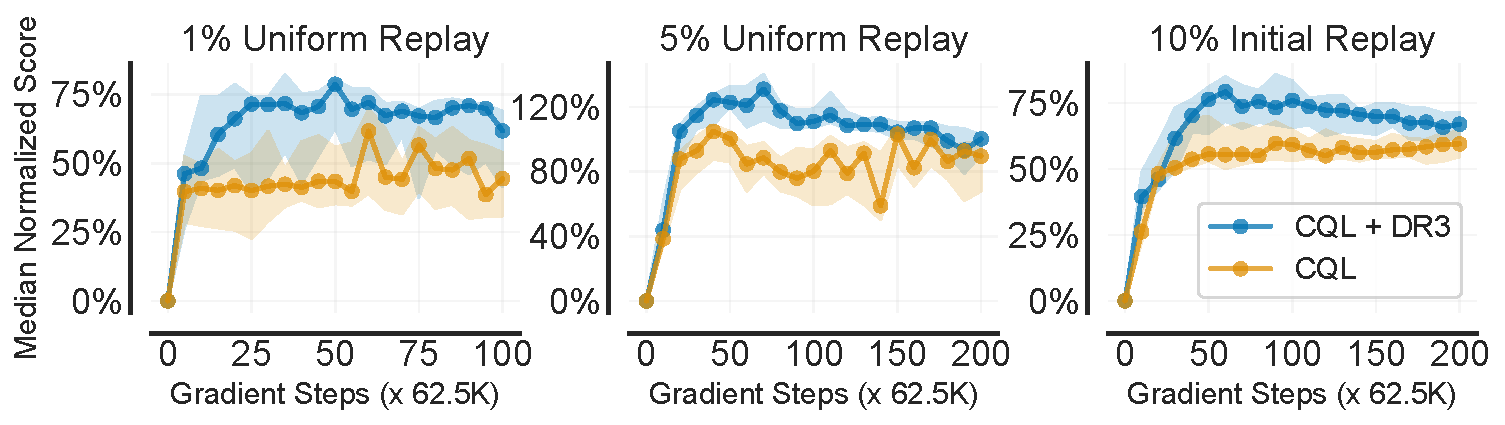
\includegraphics[width=\linewidth]{figures/atari_new/Median_cql_penalty.pdf}
% %     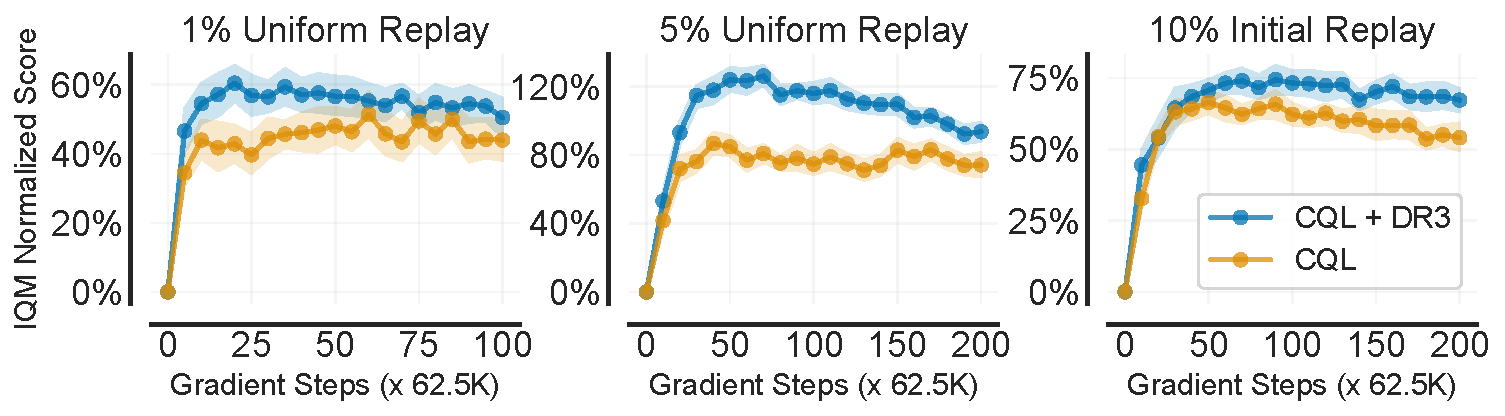
\includegraphics[width=\linewidth]{figures/atari_new/IQM_cql_penalty.pdf}
% %     % 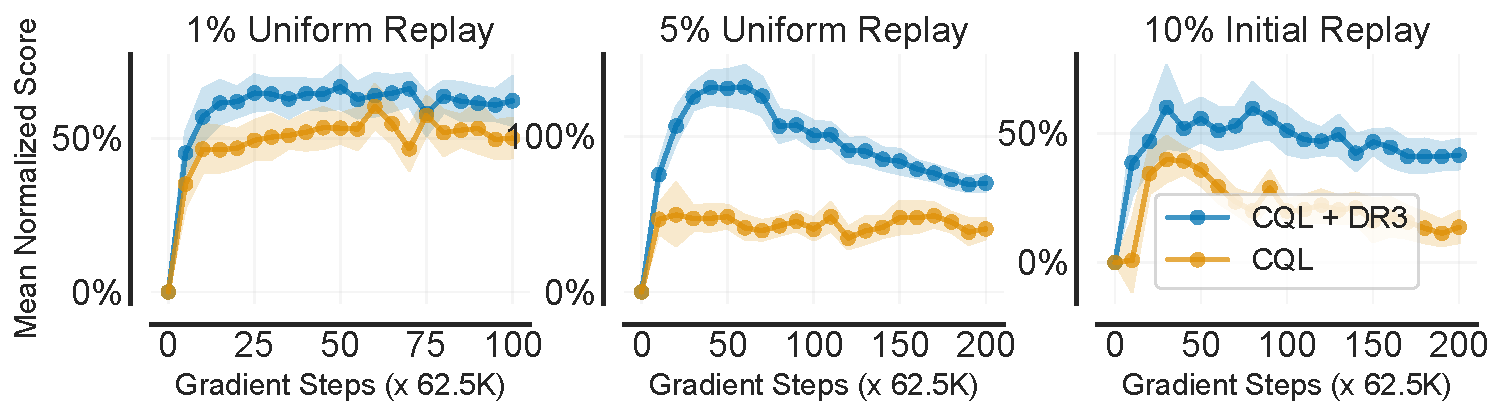
\includegraphics[width=\linewidth]{figures/atari_new/Mean_cql_penalty.pdf}
% %     % 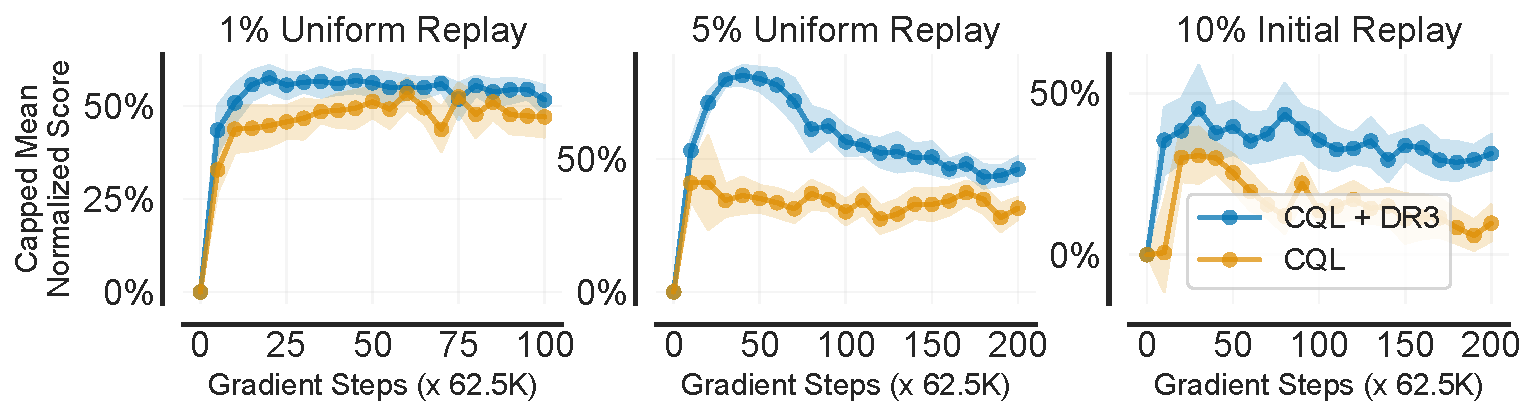
\includegraphics[width=\linewidth]{figures/atari_new/Capped_Mean_cql_penalty.pdf}
% %     \vspace{-0.65cm}
% %     \caption{Behavior Normalized Scores across 17 Atari games. We use Interquartile mean~(IQM).}
% %     \label{fig:atari_5_percent}
% % \end{figure*}



% % \begin{figure}[t]
% %     \centering
% %     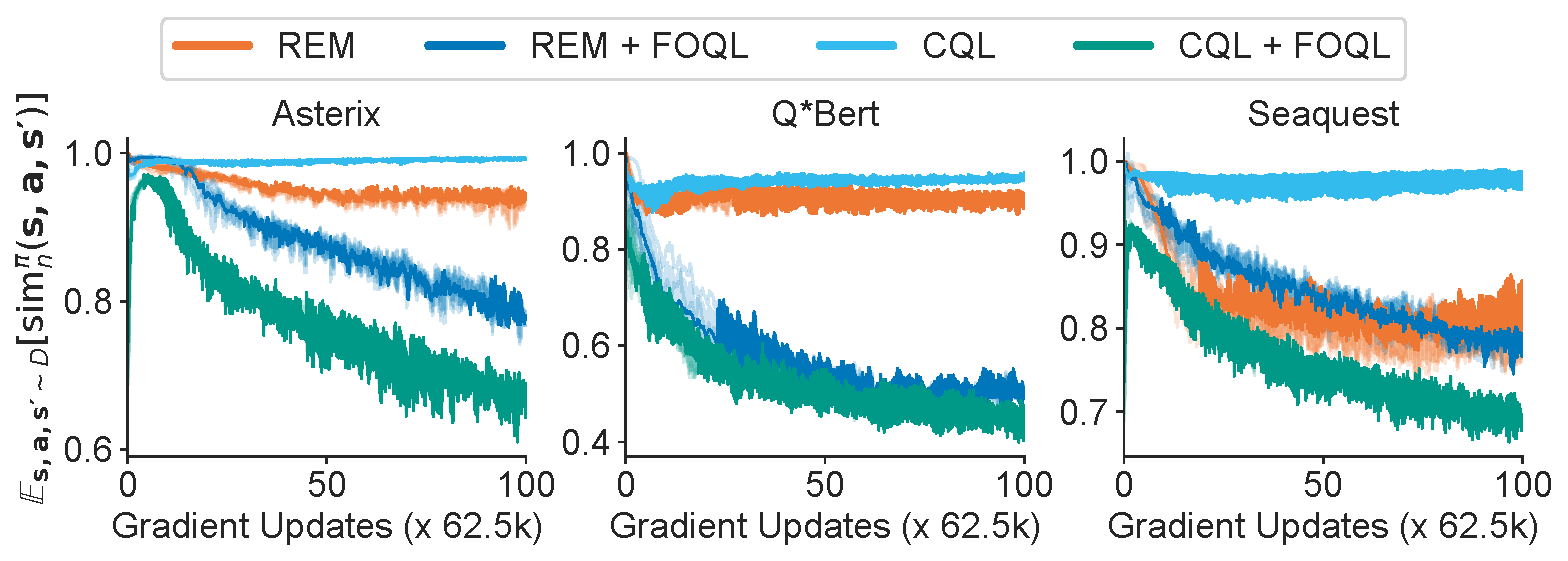
\includegraphics[width=\linewidth]{atari/norm_3_games_cql_rem.pdf}
% %     \vspace{-0.65cm}
% %     \caption{In addition to minimizing unnormalized similarities~($\simunnorm(\bs, \ba, \bs')$), \methodname\ attains much lower normalized similarities as compared to CQL and REM. The results are shown for training with 5\% DQN replay dataset averaged over 5 seeds.}\label{fig:atari_3_cosine}
% %     \vspace{-0.5cm}
% % \end{figure}


% % \begin{figure*}[t]
% %     \centering
% %     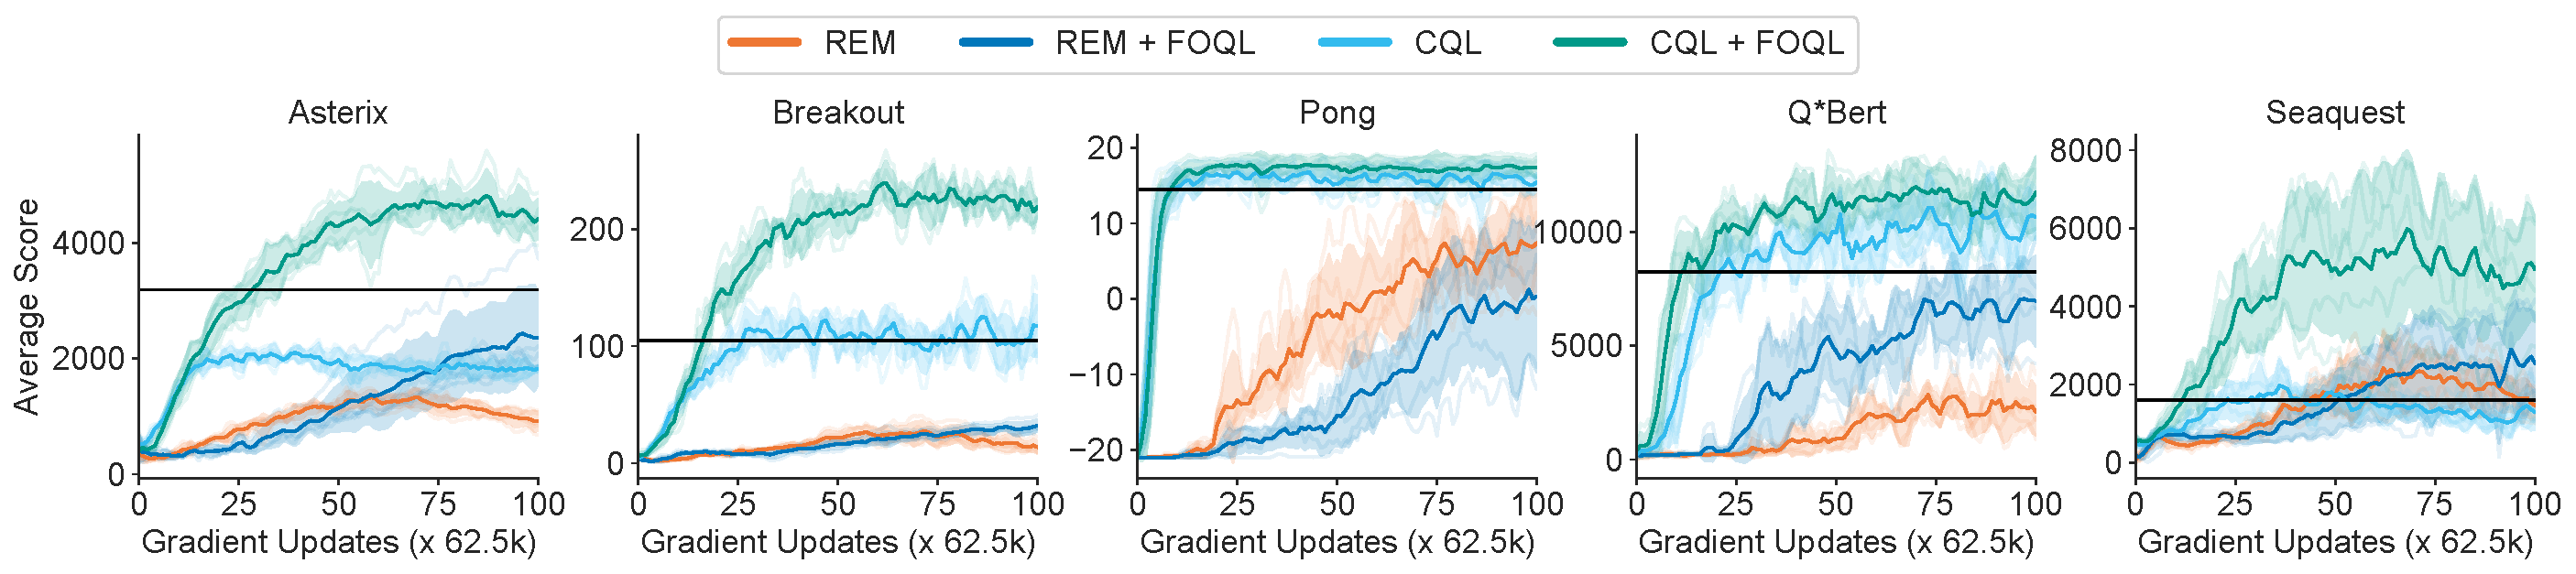
\includegraphics[width=\linewidth]{atari/5_percent_res_100.pdf}
% %     \vspace{-0.65cm}
% %     \caption{Evaluation performance of offline REM and CQL with and without \methodname\ on the 5\% DQN replay dataset~\citep{agarwal2019optimistic}. Note that the data collected during evaluation is not provided to offline agents during training. The horizontal line shows the average performance of the trajectories in entire DQN replay dataset. \methodname\ substantially improves the performance of CQL and REM as well as prevents the decay in performance of REM with more gradient updates on \textsc{Seaquest} and \textsc{Asterix}. For \textsc{Pong}, training for longer~(12.5 million updates) results in improved score for REM + \methodname\ over REM.}
% %     \label{fig:atari_5_percent}
% % \end{figure*}


% % \begin{table*}[t]
% %     \centering
% %     \caption{Normalized returns on sub-sampled Atari DQN Replay datasets~\citep{agarwal2019optimistic}. A random policy is provided a normalized score of zero while the average performance of the trajectories in the entire DQN replay dataset is assigned a normalized score of 100. We report results based on 6.5 million gradient updates with batch size of 32 for the 1\% setting and 12.5 million gradient updates for the 5\% and 10\% settings. The individual scores and learning curves for all the 17 games are provided in the Appendix~\ref{app:atari_results}.}
% %     \label{tab:cql_res}
% %     \vspace{0.2cm}
% % \begin{tabular}{cccccc}
% % \toprule
% % %%AK.1.26: maybe we want to name the average performance as Stability coefficient or something like that but thats a minor point
% % \multirow{2}{*}{DQN Replay Setting} & Normalized Score Metric & \multicolumn{2}{c}{Average Performance}   & \multicolumn{2}{c}{Maximum Performance} \\
% % & (17 games) & CQL & CQL + \methodname & CQL & CQL + \methodname \\
% % \midrule
% % 1\% replay &  Median & 43.3 & \textbf{71.0} & 73.2 & \textbf{96.3} \\
% % (uniformly sampled) & Mean & 50.7 & \textbf{60.9} & 74.4 & \textbf{84.6}  \\
% % \midrule
% % {5\% replay} & Median  & 84.6 & \textbf{104.9} & 127.8 & \textbf{150.7} \\
% % (uniformly sampled)  & Mean & 43.3 & \textbf{97.2} &  139.5 & \textbf{189.5}  \\
% % \midrule
% % {10\% replay} & Median  & 53.4 &  \textbf{69.9} & 73.3 & \textbf{97.2} \\
% % (initial exploration data) & Mean & 21.8 & \textbf{49.6} &  79.4 & \textbf{140.0}  \\
% % \bottomrule
% % \end{tabular}
% % \end{table*}

% %% Final Performance CQL vs Penalty
% % -----DR3+CQL-----
% % *****Median*****
% % 1% data
% % Median 61.8 [41.6 69. ]
% % 5% data
% % Median 100.2 [ 90.6 102.7]
% % 10% data
% % Median 67.0 [62.1 71.4]
% % *****IQM*****
% % 1% data
% % IQM 50.5 [44.9 56.1]
% % 5% data
% % IQM 93.6 [88. 99.]
% % 10% data
% % IQM 67.3 [63.2 71.4]
% % -----CQL-----
% % *****Median*****
% % 1% data
% % Median 44.4 [30.9 54. ]
% % 5% data
% % Median 89.6 [67.9 98.2]
% % 10% data
% % Median 59.6 [54.6 64.4]
% % *****IQM*****
% % 1% data
% % IQM 44.0 [38.1 49.8]
% % 5% data
% % IQM 74.2 [67.3 81.4]
% % 10% data
% % IQM 54.1 [49.5 59.3]

% %% Final performance REM vs REM+penalty
% % -----DR3+REM-----
% % *****Median*****
% % 1% data
% % Median 13.1 [10.  18.4]
% % 5% data
% % Median 72.4 [65.7 81.1]
% % 10% data
% % Median 72.4 [65.7 81.1]
% % *****IQM*****
% % 1% data
% % IQM 13.4 [11.  16.4]
% % 5% data
% % IQM 77.2 [71.4 83.9]
% % 10% data
% % IQM 77.2 [71.4 83.9]
% % -----REM-----
% % *****Median*****
% % 1% data
% % Median -0.0 [-0.7  0.1]
% % 5% data
% % Median 24.9 [14.5 29. ]
% % 10% data
% % Median 24.9 [14.5 29. ]
% % *****IQM*****
% % 1% data
% % IQM -0.1 [-0.7  0.6]
% % 5% data
% % IQM 23.5 [19.9 27.3]
% % 10% data
% % IQM 23.5 [19.9 27.3]


% % REM vs REM + penalty Average performance (stability)
% % -----DR3+REM-----
% % *****Median*****
% % 1% data
% % Median 11.7
% % 5% data
% % Median 52.5
% % 10% data
% % Median 63.9
% % *****IQM*****
% % 1% data
% % IQM 12.4
% % 5% data
% % IQM 53.5
% % 10% data
% % IQM 67.8
% % -----REM-----
% % *****Median*****
% % 1% data
% % Median 3.1
% % 5% data
% % Median 18.8
% % 10% data
% % Median 47.7
% % *****IQM*****
% % 1% data
% % IQM 3.4
% % 5% data
% % IQM 21.1
% % 10% data
% % IQM 47.9

% % FInal performance (scaled via random scores and CQL is 100\% for IUP comparison):
% % Asterix 256.6
% % BeamRider 18.6
% % Breakout 176.3
% % DemonAttack 228.0
% % DoubleDunk 133.5
% % Enduro 115.2
% % IceHockey 51.7
% % Jamesbond 310.8
% % MsPacman 131.5
% % Pong 105.5
% % Qbert 114.4
% % RoadRunner 100.0
% % Seaquest 366.6
% % SpaceInvaders 322.8
% % WizardOfWor 80.3
% % YarsRevenge 75.7
% % Zaxxon 485.6



% % \begin{table*}[t]
% %     \centering
% %     \caption{Normalized returns on sub-sampled Atari DQN replay datasets~\citep{agarwal2019optimistic}. The individual scores and learning curves for all the 17 games are provided in the Appendix~\ref{app:atari_results}. When combined with REM, we used a coefficient of $\alpha = 0.001$ to show the robustness of \methodname\ across different datasets. \color{red}{Merge the two tables somehow to save space.}}
% %     \label{tab:rem_res}
% %     \vspace{0.2cm}
% % \begin{tabular}{cccccc}
% % \toprule
% % %%AK.1.26: maybe we want to name the average performance as Stability coefficient or something like that but thats a minor point
% % \multirow{2}{*}{DQN Replay Setting} & Normalized Score Metric & \multicolumn{2}{c}{Average Performance}   & \multicolumn{2}{c}{Maximum Performance} \\
% % & (17 games) & REM & REM + \methodname & REM & REM + \methodname \\
% % \midrule
% % 1\% replay &  Median & 4.7 & \textbf{19.3} & 25.5 & \textbf{42.5} \\
% % (uniformly sampled) & Mean & -1.8 & \textbf{47.2} &  72.4 & \textbf{100.2}  \\
% % \midrule
% % {5\% replay} & Median  & 27.4 & \textbf{58.5} & 88.8 & \textbf{99.8} \\
% % (uniformly sampled)  & Mean & 40.9 & \textbf{84.7} &  141.1 & \textbf{165.8}  \\
% % \midrule
% % {10\% replay} & Median  & 50.7 &  \textbf{68.5} & 107 & \textbf{108.5} \\
% % (initial exploration data) & Mean & 63.7 & \textbf{84.4} &  136.5 & \textbf{140.7}  \\
% % \bottomrule
% % \end{tabular}
% % \end{table*}

% %% Final Performance CQL vs Penalty
% % -----DR3+CQL-----
% % *****Median*****
% % 1% data
% % Median 61.8 [41.6 69. ]
% % 5% data
% % Median 100.2 [ 90.6 102.7]
% % 10% data
% % Median 67.0 [62.1 71.4]
% % *****IQM*****
% % 1% data
% % IQM 50.5 [44.9 56.1]
% % 5% data
% % IQM 93.6 [88. 99.]
% % 10% data
% % IQM 67.3 [63.2 71.4]
% % -----CQL-----
% % *****Median*****
% % 1% data
% % Median 44.4 [30.9 54. ]
% % 5% data
% % Median 89.6 [67.9 98.2]
% % 10% data
% % Median 59.6 [54.6 64.4]
% % *****IQM*****
% % 1% data
% % IQM 44.0 [38.1 49.8]
% % 5% data
% % IQM 74.2 [67.3 81.4]
% % 10% data
% % IQM 54.1 [49.5 59.3]

% % CQL  vs CQL + penalty Average performance (stability)
% % -----DR3+CQL-----
% % *****Median*****
% % 1% data
% % Median 63.7
% % 5% data
% % Median 102.6
% % 10% data
% % Median 65.2
% % *****IQM*****
% % 1% data
% % IQM 52.6
% % 5% data
% % IQM 102.4
% % 10% data
% % IQM 65.2
% % -----CQL-----
% % *****Median*****
% % 1% data
% % Median 42.5
% % 5% data
% % Median 81.4
% % 10% data
% % Median 52.1
% % *****IQM*****
% % 1% data
% % IQM 42.8
% % 5% data
% % IQM 72.3
% % 10% data
% % IQM 56.3


% % \begin{table*}[t]
% %     \centering
% %     \caption{\small{Performance of REM, REM + \methodname after 6.5M gradient steps for the 1\% setting and 12.5M gradient steps for the 5\%, 10\% settings. Individual scores for all 17 games are provided in the Appendix~\ref{app:atari_results}.}}
% %     \label{tab:rem_res}
% %     \vspace{0.2cm}
% % \begin{tabular}{cccccc}
% % \toprule
% % \multirow{2}{*}{\textbf{Data}} & \textbf{Metric} & \multicolumn{2}{c}{\textbf{Last iteration score}}   & \multicolumn{2}{c}{\textbf{Stability score}} \\
% % & (17 games) & REM & REM + \methodname & REM & REM + \methodname \\
% % \midrule
% % 1\% &  Median & 0.0 & \textbf{13.1} & 3.1 & \textbf{11.7} \\
% %  & IQM & -0.1 & \textbf{13.4} & 3.4 & \textbf{12.4}  \\
% % \midrule
% % 5\% & Median  & 24.9 & \textbf{72.4} & 18.8 & \textbf{52.5} \\
% %  & IQM & 23.5 & \textbf{77.2} &  21.1 & \textbf{53.5}  \\
% % \midrule
% % 10\% & Median & 24.9 &  \textbf{72.4} & 47.7 & \textbf{63.9} \\
% %  & IQM & 23.5 & \textbf{77.4} &  47.9 & \textbf{67.8}  \\
% % \bottomrule
% % \end{tabular}
% % \end{table*}



% % REM vs REM + penalty Average performance (stability)
% % -----DR3+REM-----
% % *****Median*****
% % 1% data
% % Median 11.7
% % 5% data
% % Median 52.5
% % 10% data
% % Median 63.9
% % *****IQM*****
% % 1% data
% % IQM 12.4
% % 5% data
% % IQM 53.5
% % 10% data
% % IQM 67.8
% % -----REM-----
% % *****Median*****
% % 1% data
% % Median 3.1
% % 5% data
% % Median 18.8
% % 10% data
% % Median 47.7
% % *****IQM*****
% % 1% data
% % IQM 3.4
% % 5% data
% % IQM 21.1
% % 10% data
% % IQM 47.9

% %% Final performance REM vs REM+penalty
% % -----DR3+REM-----
% % *****Median*****
% % 1% data
% % Median 13.1 [10.  18.4]
% % 5% data
% % Median 72.4 [65.7 81.1]
% % 10% data
% % Median 72.4 [65.7 81.1]
% % *****IQM*****
% % 1% data
% % IQM 13.4 [11.  16.4]
% % 5% data
% % IQM 77.2 [71.4 83.9]
% % 10% data
% % IQM 77.2 [71.4 83.9]
% % -----REM-----
% % *****Median*****
% % 1% data
% % Median -0.0 [-0.7  0.1]
% % 5% data
% % Median 24.9 [14.5 29. ]
% % 10% data
% % Median 24.9 [14.5 29. ]
% % *****IQM*****
% % 1% data
% % IQM -0.1 [-0.7  0.6]
% % 5% data
% % IQM 23.5 [19.9 27.3]
% % 10% data
% % IQM 23.5 [19.9 27.3]

% % \begin{table*}[t]
% %     \centering
% %     \caption{\small{Performance of REM, REM + \methodname after 6.5M gradient steps for the 1\% setting and 12.5M gradient steps for the 5\%, 10\% settings. Individual scores for all 17 games are provided in the Appendix~\ref{app:atari_results}.}}
% %     \label{tab:rem_res}
% %     \vspace{0.2cm}
% % \begin{tabular}{cccccc}
% % \toprule
% % \multirow{2}{*}{\textbf{Data}} & \textbf{Metric} & \multicolumn{2}{c}{\textbf{Last iteration score}}   & \multicolumn{2}{c}{\textbf{Stability score}} \\
% % & (17 games) & REM & REM + \methodname & REM & REM + \methodname \\
% % \midrule
% % 1\% &  Median & 0.0 & \textbf{13.1} & 3.1 & \textbf{11.7} \\
% %  & IQM & -0.1 & \textbf{13.4} & 3.4 & \textbf{12.4}  \\
% % \midrule
% % 5\% & Median  & 24.9 & \textbf{72.4} & 18.8 & \textbf{52.5} \\
% %  & IQM & 23.5 & \textbf{77.2} &  21.1 & \textbf{53.5}  \\
% % \midrule
% % 10\% & Median & 24.9 &  \textbf{72.4} & 47.7 & \textbf{63.9} \\
% %  & IQM & 23.5 & \textbf{77.4} &  47.9 & \textbf{67.8}  \\
% % \bottomrule
% % \end{tabular}
% % \end{table*}

% % \begin{wrapfigure}{r}{0.57\textwidth}
% %     \centering
% %     \vspace{-5pt}
% %     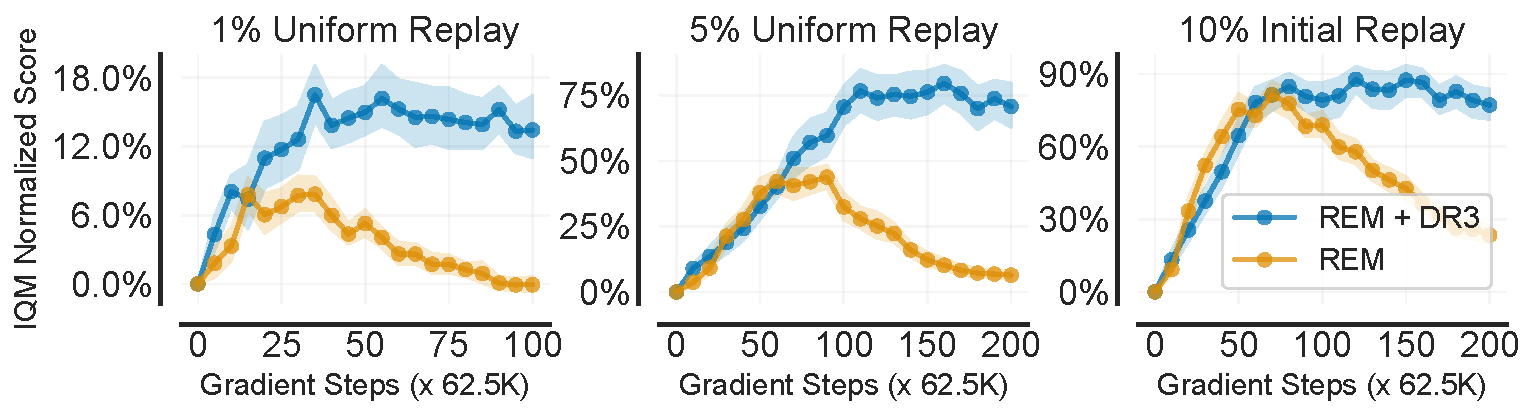
\includegraphics[width=0.99\linewidth]{figures/atari_new/IQM_rem_penalty.pdf}
% %     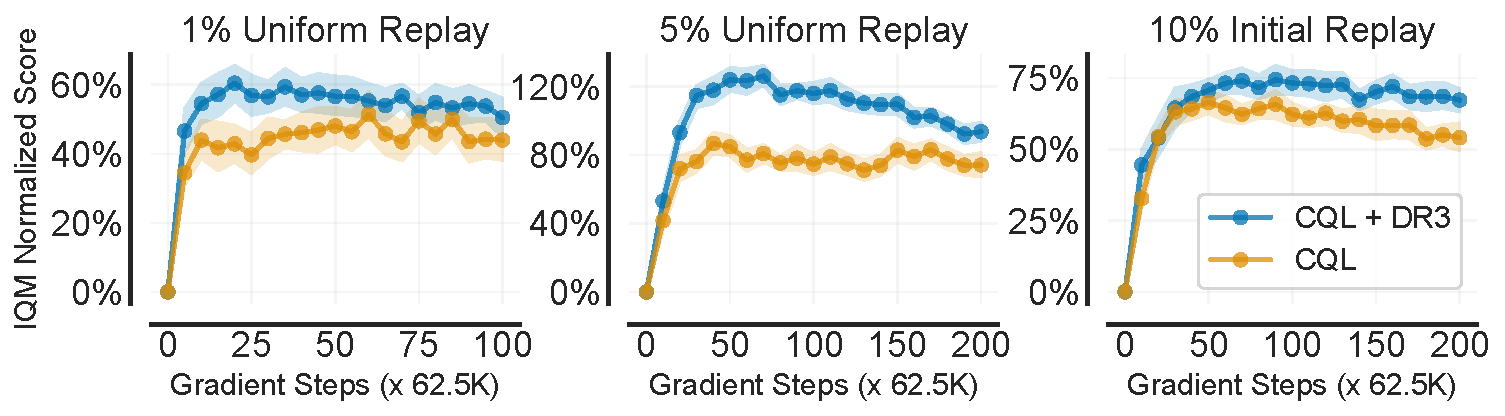
\includegraphics[width=0.99\linewidth]{figures/atari_new/IQM_cql_penalty.pdf}
% %     \vspace{-0.25in}
% %     \caption{\small{\textbf{Average normalized performance across 17 Atari games for REM + \methodname\ (top), CQL + \methodname\ (bottom)} over the course of training with different datasets. x-axis represents \emph{gradient steps}; no new data is collected. While na\"ive REM suffers from a degradation in performance with more training, REM + \methodname\ not only remains generally stable with more training, but also attains higher final performance. CQL + \methodname\ attains higher performance than CQL. As recommended by \citet{agarwal2021precipice}, we report interquartile Mean (IQM) with stratified bootstrap 95\% CIs as shaded regions.}}
% %     \label{fig:atari_all_combined}
% %     \vspace{-0.45cm}
% % \end{wrapfigure}
% \textbf{{Offline RL on Atari 2600 games.}} We compare \methodname\ to prior offline RL methods on a set of offline Atari datasets of varying sizes and quality, akin to \citet{agarwal2019optimistic, kumar2021implicit}. We evaluated on three datasets: \textbf{(1)} 1\% and 5\% samples drawn uniformly at random from DQN replay; \textbf{(2)} a dataset with more suboptimal data consisting of the first 10\% samples observed by an online DQN. Following \citet{agarwal2021precipice}, we report the interquartile mean~(IQM) normalized scores across 17 games over the course of training in Figure~\ref{fig:atari_all_combined} and report the IQM average performance in Table~\ref{tab:cql_res}. Observe that combining \methodname\ with modern offline RL methods (CQL, REM) attains the best final and average performance across the 17 Atari games tested on, directly improving upon prior methods
% across all the datasets. When \methodname\ is used in conjunction with REM, it prevents unlearning and performance degradation with more training. CQL + \methodname\ improves by \textbf{20\%} over CQL on final performance and attains \textbf{25\%} better average performance. We also compare \methodname\ to the $\mathrm{srank}(\Phi)$ penalty proposed to counter rank collapse~\citep{kumar2021implicit}. Directly taking median normalized score improvements reported by \citet{kumar2021implicit}, CQL + \methodname\ improves by over \textbf{2x} (31.5\%) over na\"ive CQL relative to the srank penalty~(14.1\%), indicating DR3's efficacy.
% % this $\text{srank}$ penalty only attains a median improvement of 14.1\% over na\"ive CQL, whereas CQL + \methodname\ attains a median improvement of \textbf{31.5\%} over CQL. Thus, CQL + \methodname\ improves by over \textbf{2x} relative to the srank penalty, indicating DR3's efficacy.
% % This indicates that by directly addressing the adverse impacts of implicit regularization, \methodname\ can substantially improve upon prior methods that only address its symptoms.  

% %Notably, REM performs similar to a random policy in terms of average performance on the 1\%  setting, which is significantly improved by \methodname.
% %%SL.2.1: I think we can cut this last sentence, and instead focus on the more positive takeaways.

% % To evaluate whether the improvements from \methodname\ stem from penalizing unnormalized similarities $\simunnorm(\bs, \ba, \bs')$, we also compare \methodname\ to penalizing (1) $\simnorm(\bs, \ba, \bs')$, or (2) feature norms~($\|\phi(\bs)\|_2$) on the 5\% dataset on 5 games. The full results, shown in Appendix~\ref{}, confirms that both of these penalties perform substantially worse than \methodname, aligned with our theoretical analysis about effectiveness of \methodname~(Section~\ref{sec:method_analysis}).

% %%SL.2.1: This last phrase is without context. What question is it trying to answer? What is the motivation? Start with a sentence of motivation or a question, then evidence, then answer. Something like: Is [whatever] true? To answer this question, we can [do something]. The full results, shown in [where], indicate [something]. This suggests that [something].
% \begin{wrapfigure}{r}{0.42\textwidth}
% \small \begin{center}
% \vspace{-15pt}
% 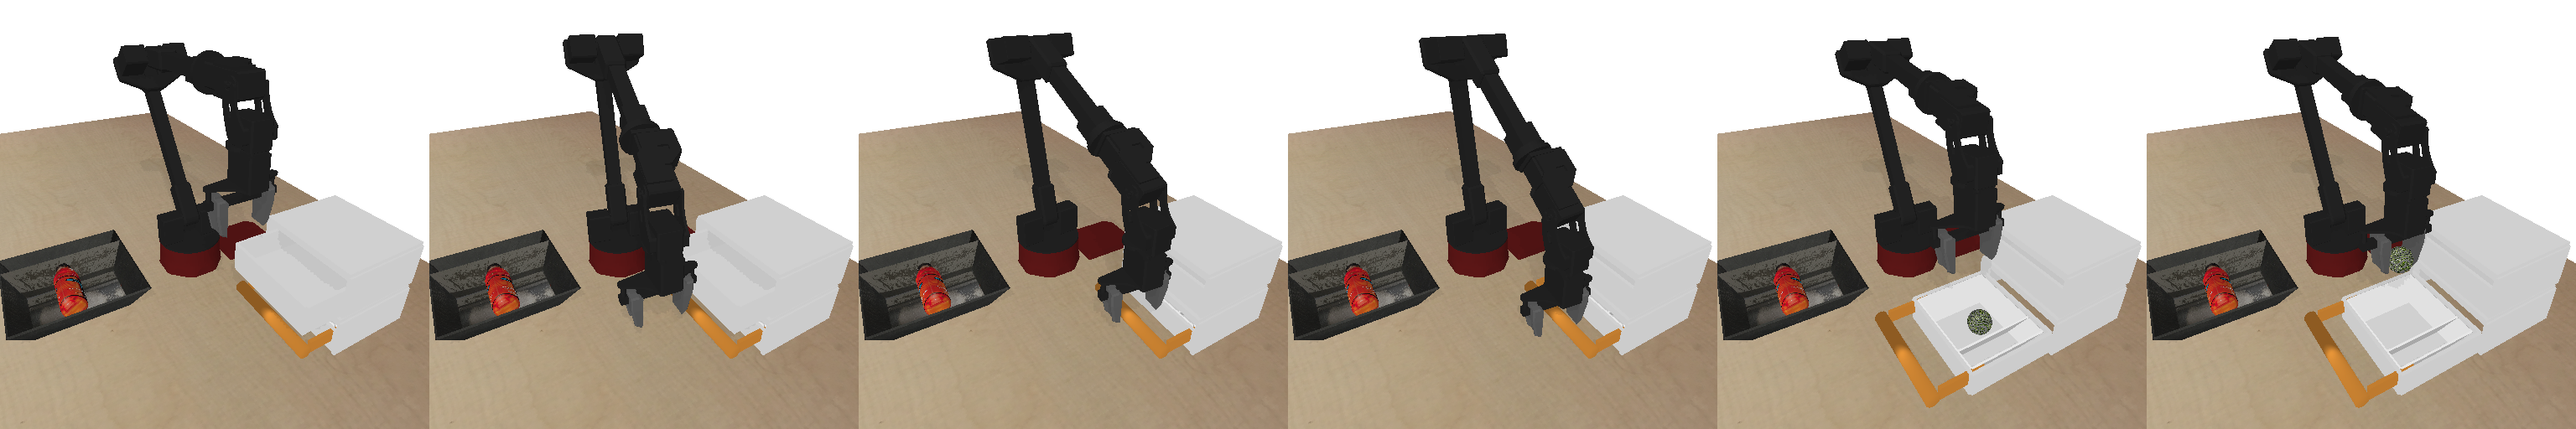
\includegraphics[width=0.99\linewidth]{figures/close_open_grasp (1).png}
% 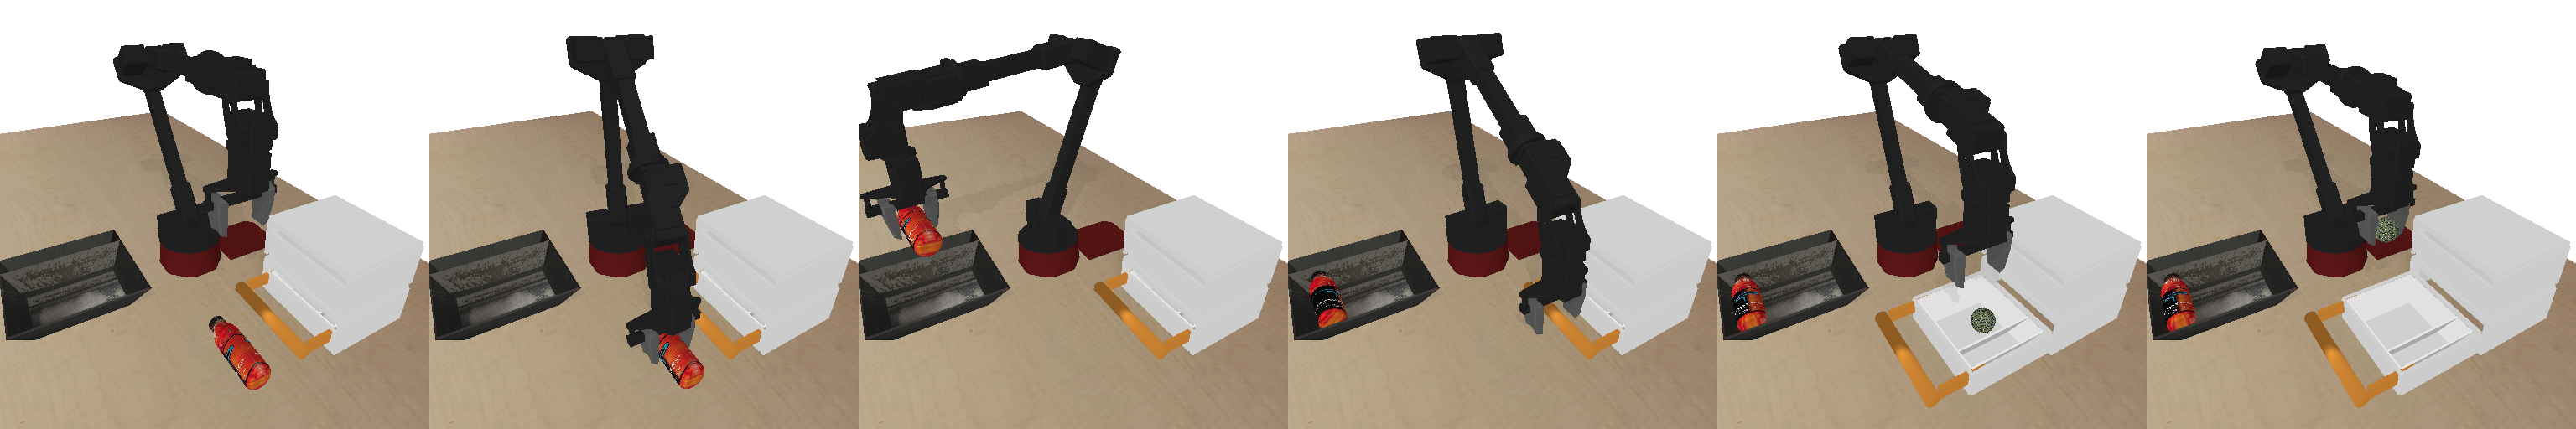
\includegraphics[width=0.99\linewidth]{figures/pickplace_open_grasp.png}
% \vspace{-20pt}
% \end{center}
% \end{wrapfigure}
% \textbf{{Offline RL on robotic manipulation from}} \textbf{{images.}} Next, we aim to evaluate the efficacy of \methodname\ on two image-based robotic manipulation tasks~\citep{singh2020cog}~(visualized on the right) that require composition of skills (e.g., opening a drawer, closing a drawer, picking an obstructive object, placing an object, etc.) over extended horizons using only a sparse 0-1 reward. 
% As shown in Figure~\ref{fig:cog_figure}, combining \methodname\ with COG not only improves over COG, but also learns faster and attains a better average performance.

% \begin{table}[t]
%     \centering
% \fontsize{8}{8}\selectfont
%     \centering
%     \vspace{-0.1cm}
%     \caption{\footnotesize{IQM normalized average performance (training stability) across 17 games, with 95\% CIs in parenthesis, after 6.5M gradient steps for the 1\% setting and 12.5M gradient steps for the 5\%, 10\% settings. Individual performances reported in Tables~\ref{tab:cql_dqn_1}-\ref{tab:rem_dqn_10}. \methodname\ improves the stability over both CQL and REM.  }}%As recommended by \citet{agarwal2021precipice}, we report IQM with 95\% CIs.}
%     \label{tab:cql_res}
%     \vspace{-0.1cm}
% \begin{tabular}{lcccc}
% \toprule
% % \multirow{2}{*}{\textbf{Data}}  & \multicolumn{4}{c}{\textbf{Stability performance}} \\
% Data & CQL & CQL + \methodname & REM & REM + \methodname \\
% \midrule
% 1\%   & 43.7~\ss{(39.6, 48.6)} & \textbf{56.9}~\ss{(52.5, 61.2)} & 4.0~\ss{(3.3, 4.8)} & \textbf{16.5}~\ss{(14.5, 18.6)}  \\
% \midrule
% 5\%   &  78.1~\ss{(74.5, 82.4)} & \textbf{105.7}~\ss{(101.9, 110.9)} & 25.9~\ss{(23.4, 28.8)} & \textbf{60.2}~\ss({55.8, 65.1}) \\
% \midrule
% 10\%  & 59.3~\ss{(56.4, 61.9)} & \textbf{65.8}~\ss{(63.3, 68.3)} & 53.3~\ss{(51.4, 55.3)} & \textbf{73.8}~\ss{(69.3, 78)} \\
% \bottomrule
% \vspace{-0.25in}
% \end{tabular}
% \end{table}

% \begin{figure}[t]
% % \vspace{-pt}
% \centering
% \begin{minipage}{.4\textwidth}
% % 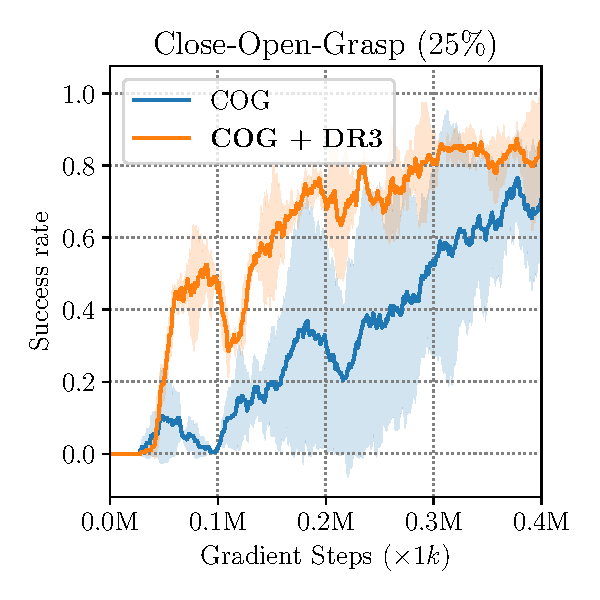
\includegraphics[width=0.49\linewidth]{figures/Widow250DoubleDrawerCloseOpenGraspNeutral-v0_cog_vs_dr3_25_v2.pdf}
% % 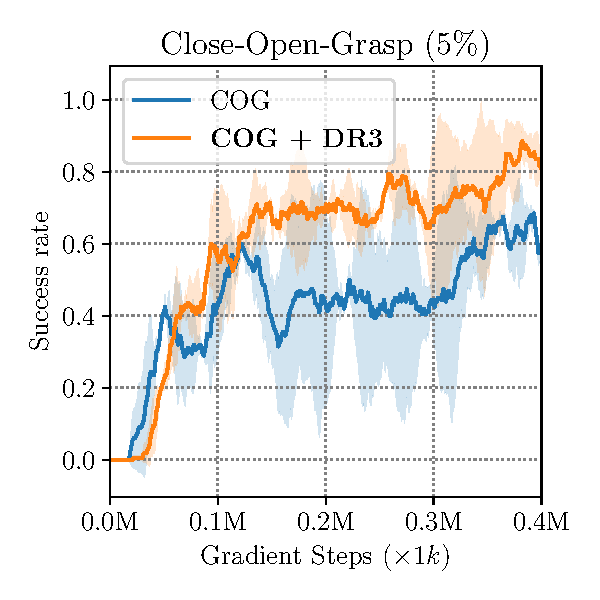
\includegraphics[width=0.49\linewidth]{figures/Widow250DoubleDrawerCloseOpenGraspNeutral-v0_cog_vs_dr3_25_v3.pdf}
% % 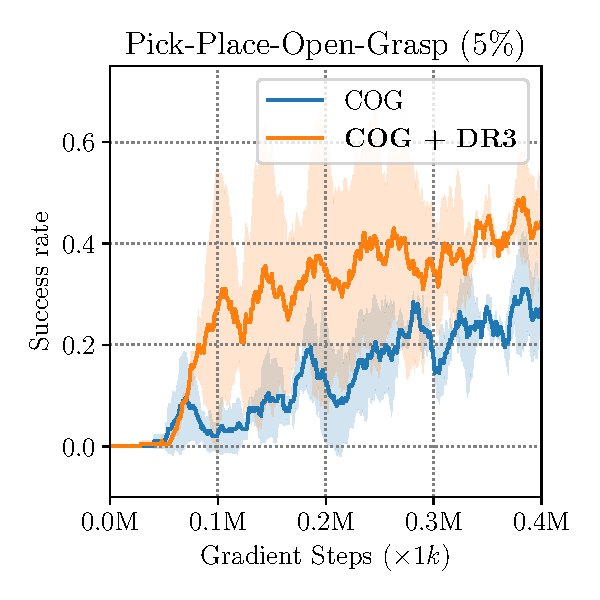
\includegraphics[width=0.49\linewidth]{figures/Widow250DoubleDrawerPickPlaceOpenGraspNeutral-v0_cog_vs_dr3_25_v4.pdf}
% % 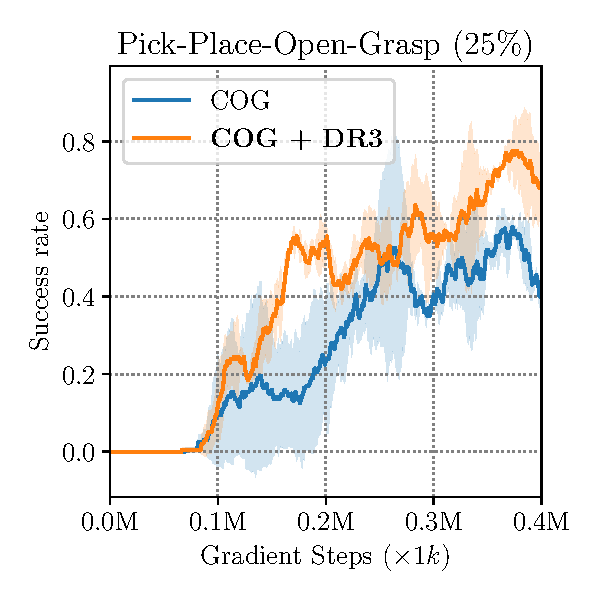
\includegraphics[width=0.49\linewidth]{figures/Widow250DoubleDrawerPickPlaceOpenGraspNeutral-v0_cog_vs_dr3_25.pdf}
% % \vspace{-10pt}
% 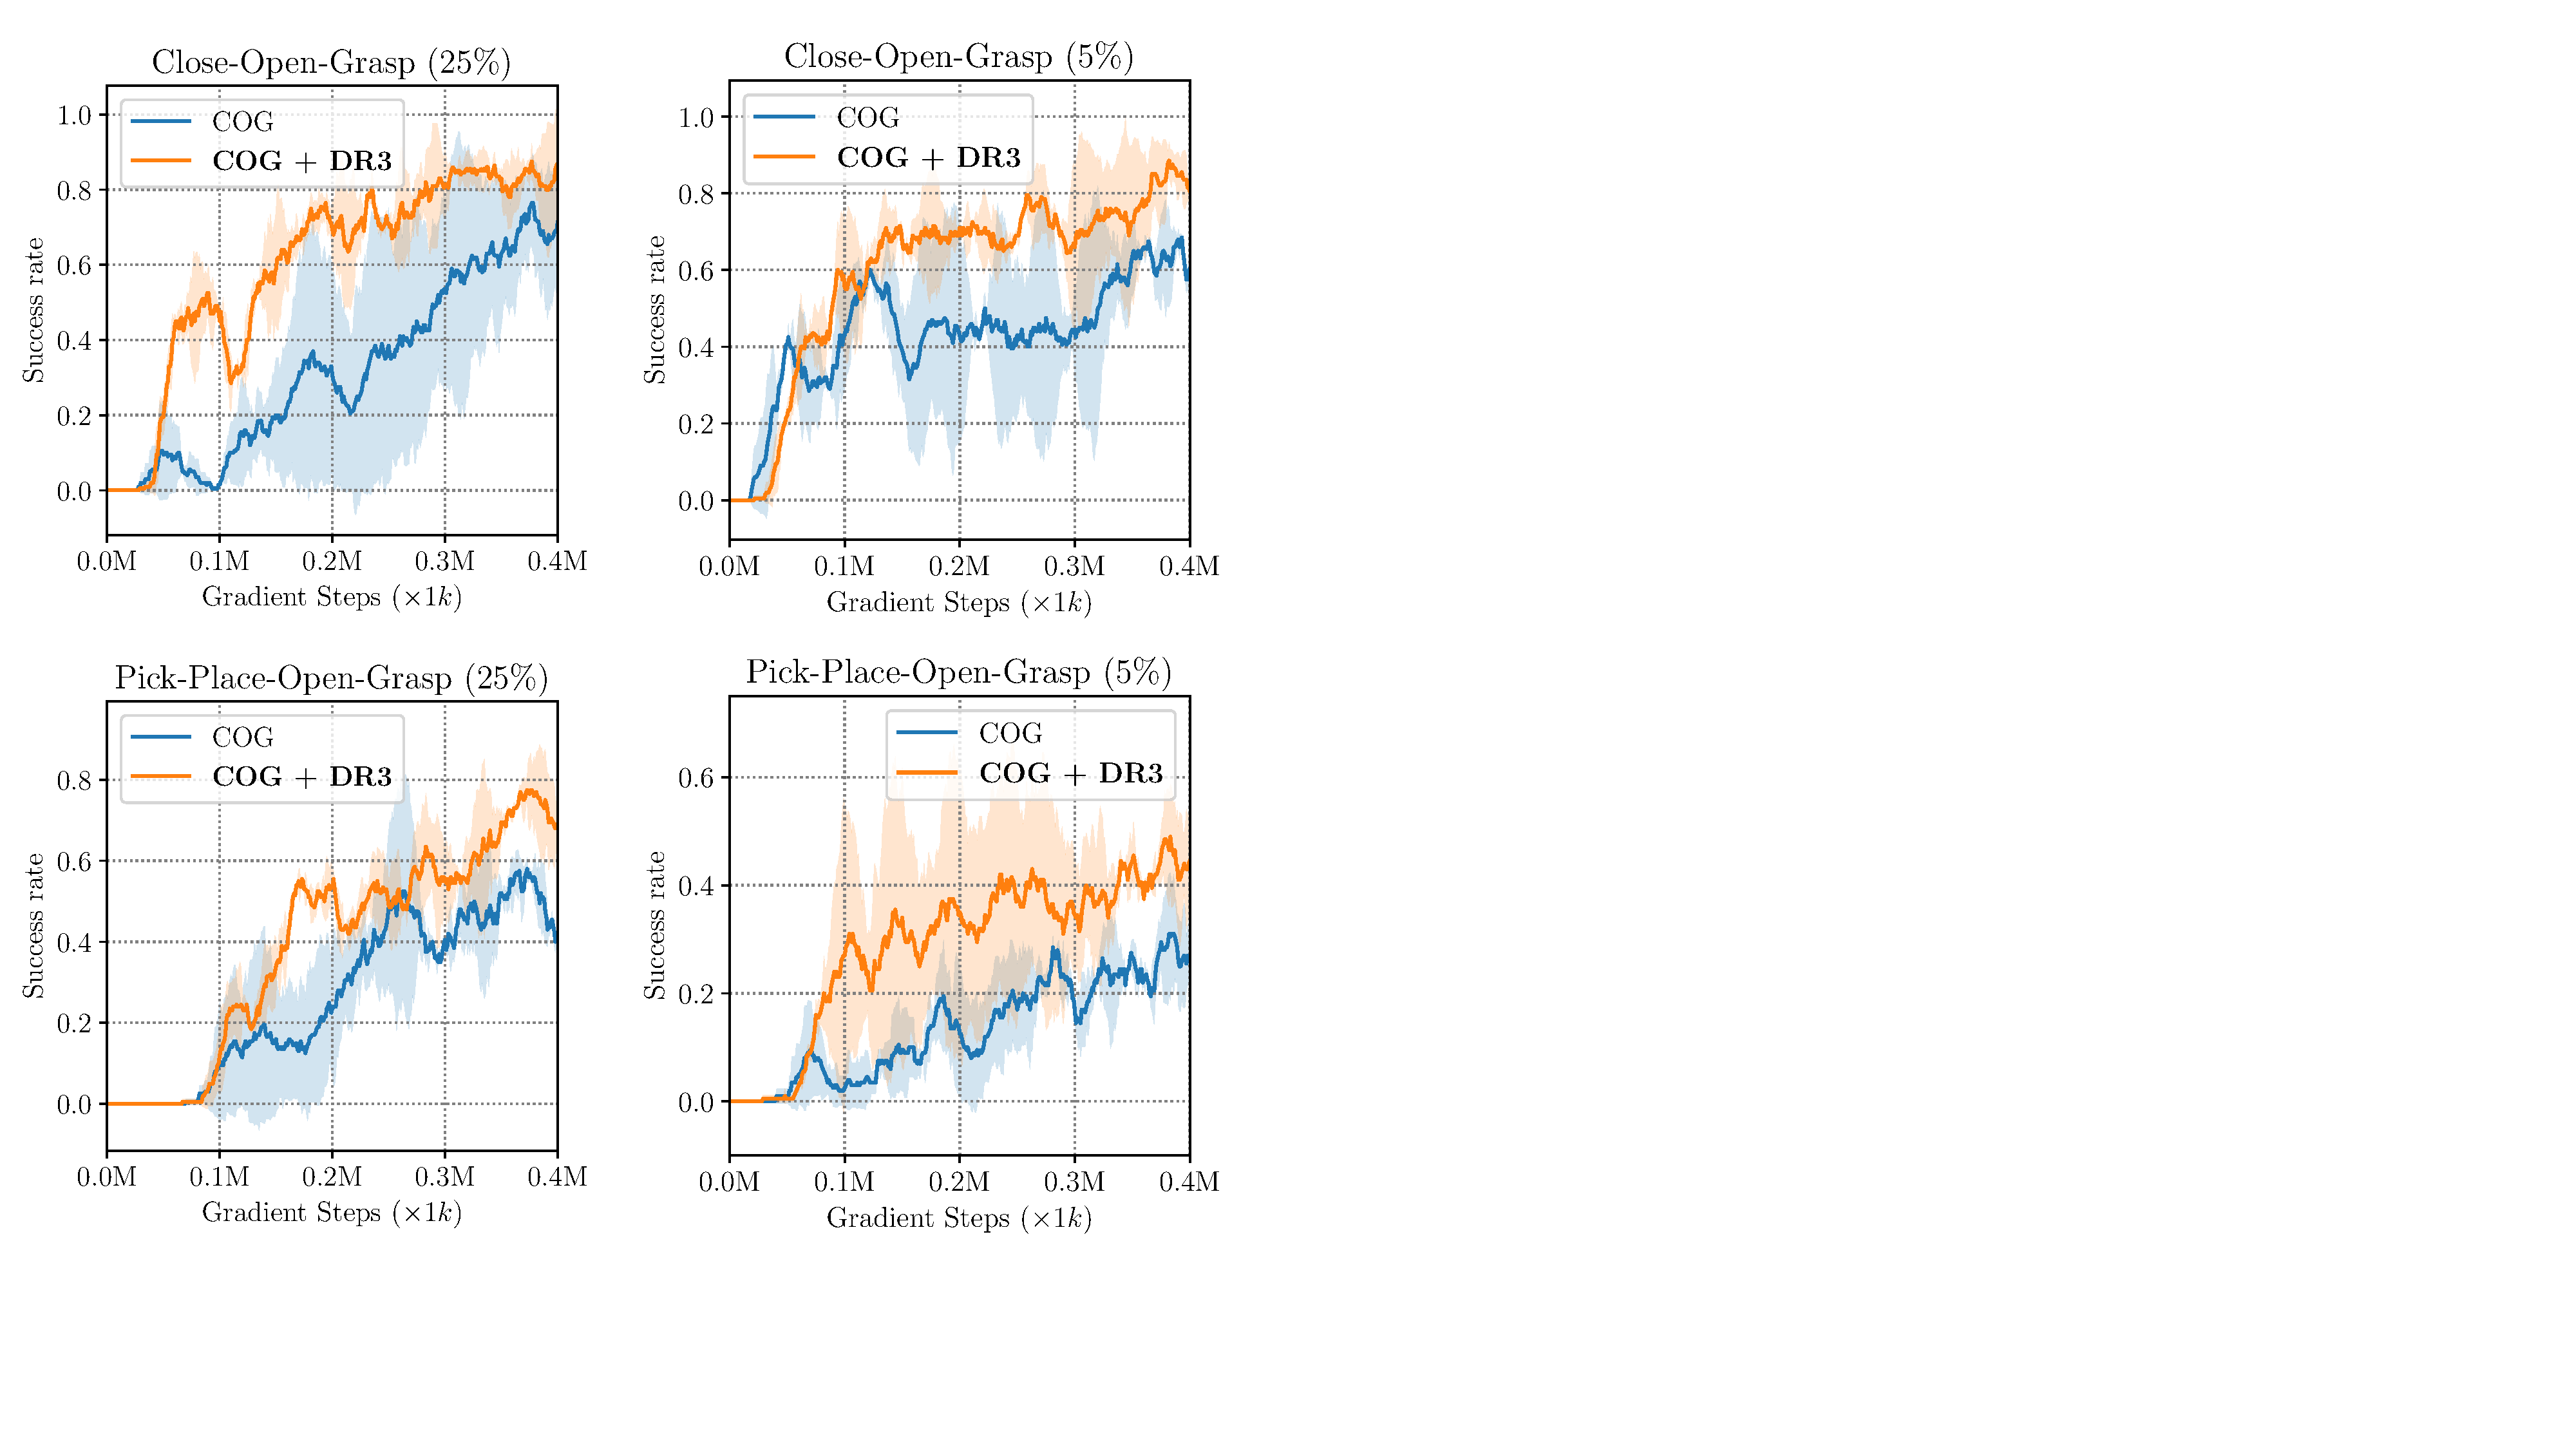
\includegraphics[width=0.96\linewidth]{figures/cog_plots.pdf}
% \vspace{-0.1in}
% \caption{\footnotesize{\textbf{Performance of \methodname\ + COG} on two manipulation tasks using only 5\% and 25\% of the data used by \citet{singh2020cog} to make these more challenging.
% COG + \methodname\  outperforms COG in training and attains higher average and final performance.}}
% \label{fig:cog_figure}
% \end{minipage}~~\vline~~
% \begin{minipage}{.56\textwidth}
%     \centering
%     % \vspace{-0.1in}
%     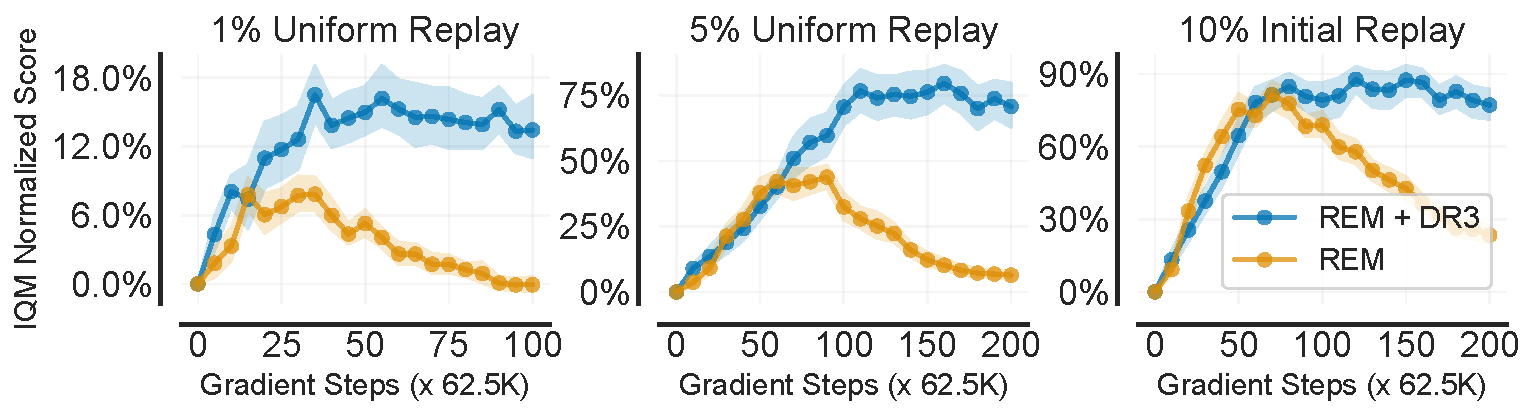
\includegraphics[width=0.99\linewidth]{figures/atari_new/IQM_rem_penalty.pdf}
%     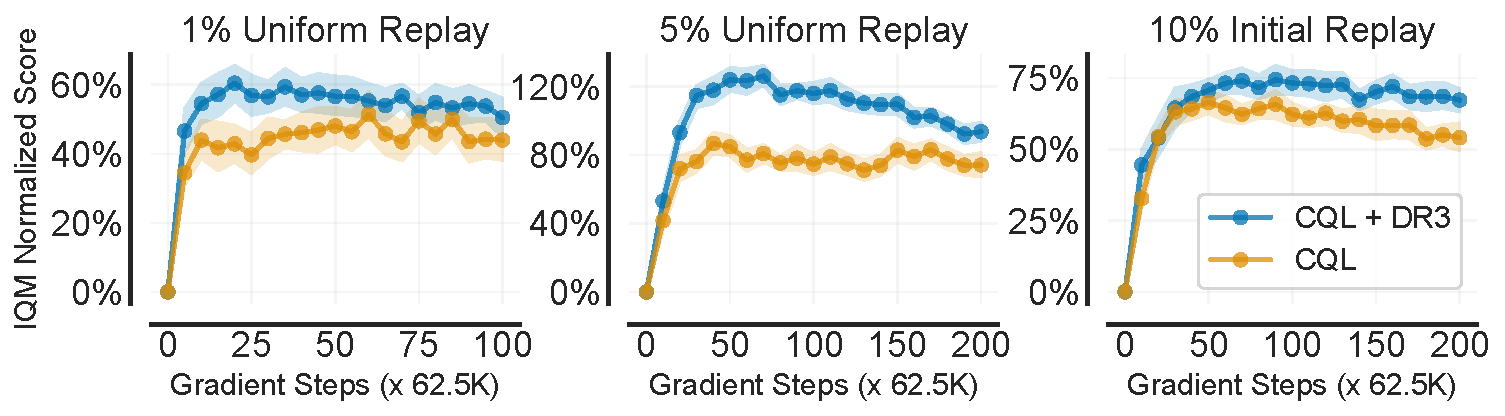
\includegraphics[width=0.99\linewidth]{figures/atari_new/IQM_cql_penalty.pdf}
%     \vspace{-0.25in}
%     \caption{\footnotesize{\textbf{Normalized performance across 17 Atari games for REM + \methodname\ (top), CQL + \methodname\ (bottom)}. x-axis represents \emph{gradient steps}; no new data is collected. While na\"ive REM suffers from a degradation in performance with more training, REM + \methodname\ not only remains generally stable with more training, but also attains higher final performance. CQL + \methodname\ attains higher performance than CQL. We report IQM with  95\% stratified bootstrap CIs~\citep{agarwal2021precipice}}.}
%     \label{fig:atari_all_combined}
% \end{minipage}
% \vspace{-0.5cm}
% \end{figure}



% % \begin{figure}[ht]
% % % \vspace{-pt}
% % \small \begin{center}
% % % \vspace{-10pt}
% % % 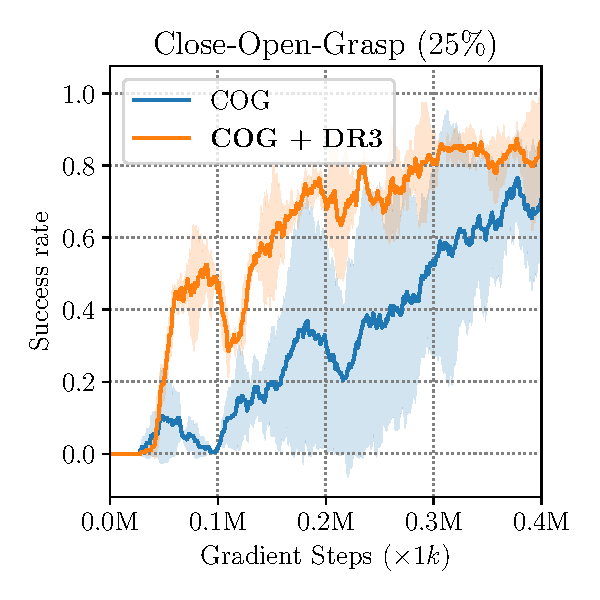
\includegraphics[width=0.49\linewidth]{figures/Widow250DoubleDrawerCloseOpenGraspNeutral-v0_cog_vs_dr3_25_v2.pdf}
% % % 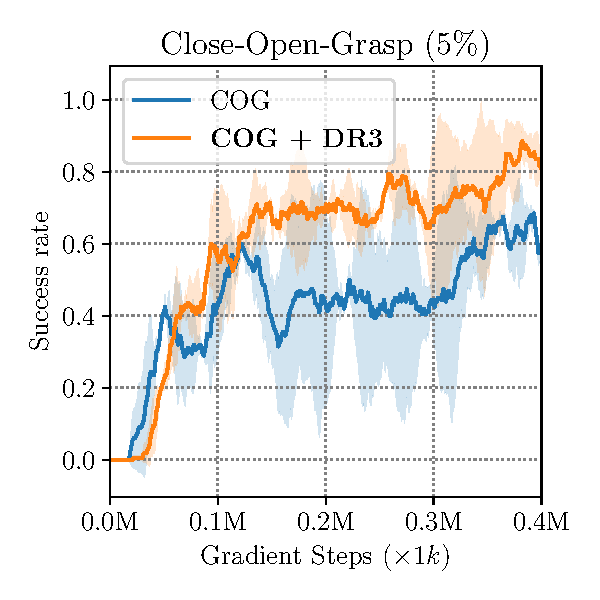
\includegraphics[width=0.49\linewidth]{figures/Widow250DoubleDrawerCloseOpenGraspNeutral-v0_cog_vs_dr3_25_v3.pdf}
% % % 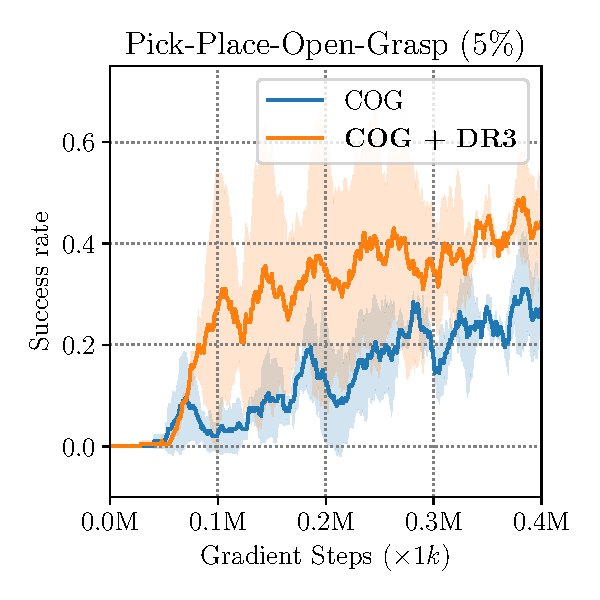
\includegraphics[width=0.49\linewidth]{figures/Widow250DoubleDrawerPickPlaceOpenGraspNeutral-v0_cog_vs_dr3_25_v4.pdf}
% % % \includegraphics[width=0.49\linewidth]{figures/Widow250DoubleDrawerPickPlaceOpenGraspNeutral-v0_cog_vs_dr3_25.pdf}
% % \includegraphics[width=0.5\linewidth]{figures/cog_plots.pdf}
% % \end{center}
% % \vspace{-15pt}
% % \caption{\small{\textbf{Performance of \methodname\ + COG} on four robotic manipulation settings with different amounts of data. As is visible, COG + \methodname\ always outperforms COG and attains higher average and final performance.}}
% % \vspace{-5pt}
% % \label{fig:cog_figure}
% % \end{figure}


% \begin{figure*}
% % \hline
%     \begin{minipage}{.5\textwidth}
%     \centering
%     \vspace{-0.01in}
%     \includegraphics[width=0.99\linewidth]{figures/rank_trends_dr3_dqn.pdf}
%     % \includegraphics[width=\linewidth]{figures/pickplace_open_grasp.png}
%     \vspace{-0.2in}
%     \caption{\footnotesize{{\textbf{Trend of effective rank,} $\mathrm{srank}(\Phi)$ of features $\Phi$ learned by the Q-function when trained with TD error (red, ``Without DR3'') and with TD error + \methodname\ (blue, ``With DR3'') on three Atari games using the 5\% dataset. Note that \methodname\ alleviates rank collapse observed by \citet{kumar2021implicit}, without explicitly aiming to. Effective rank measures the number of directions with significant singular values~(Appendix~\ref{app:rank_collapse_is_gone}).}}}
%     \label{fig:iup_is_fixed}
%     \vspace{-0.25in}
%     \end{minipage}~~\vline~~
%     \begin{minipage}{.47\textwidth}
%     % \begin{table}[t]
%     % % \vspace{-0.8cm}
%     \vspace{-0.05in}
%     \fontsize{8}{8}\selectfont
%     \centering
%     \captionof{table}{\footnotesize{\textbf{Performance of CQL, CQL + \methodname\ after 2M gradient steps with a learning rate of 3e-4} for the Q-function averaged over 4 seeds. This is training for \textbf{6x} longer compared to CQL defaults. Observe that CQL + \methodname\ outperforms CQL at 2M steps, indicating is efficacy in inducing stability. %``\texttt{med}'' stands for medium and ``\texttt{lar}'' stands for large.
%     }}
%     \label{tab:cql_d4rl}
%     \vspace{-0.1in}
%     \begin{tabular}{@{}lrr@{}}
%     \toprule
%     {\textbf{D4RL (-v0) Task}} & CQL & CQL + \methodname \\
%     \midrule
%     \texttt{kitchen-mixed} & 14.6 $\pm$ 20.5 & \textbf{37.0 $\pm$ 8.0} \\
%     \texttt{kitchen-partial} & 29.6 $\pm$ 19.6 & \textbf{43.5 $\pm$ 1.9}  \\
%     \texttt{kitchen-complete} & 22.3 $\pm$ 17.5 & 24.8 $\pm$ 15.3 \\
%     \midrule
%     \texttt{antmaze-med-diverse} & 0.7 $\pm$ 0.1 & \textbf{0.9 $\pm$ 0.1} \\
%     \texttt{antmaze-med-play} & 0.5 $\pm$ 0.4 & 0.4 $\pm$ 0.3 \\
%     \texttt{antmaze-lar-diverse} & 0.1 $\pm$ 0.0 & \textbf{0.3 $\pm$ 0.16}\\
%     \texttt{antmaze-lar-play} & 0.06 $\pm$ 0.09 & 0.1 $\pm$ 0.01 \\
%     \bottomrule
%     \end{tabular}
%     \vspace{-0.5cm}
%     \end{minipage}
% \end{figure*}
% % \hline
% % \begin{table}[t]
% % % \vspace{-0.8cm}
% % \fontsize{8}{8}
% % \centering
% % \caption{\small{Performance of CQL, CQL + \methodname\ after 2M (twice as long as prior work) gradient steps with a learning rate of 3e-4 for the Q-function averaged over 4 seeds. We also find that CQL + \methodname\ outperforms CQL at 2M steps, and is comparable to CQL when evaluated at 1M steps, which was the protocol followed originally. ``\texttt{med}'' stands for medium and ``\texttt{lar}'' stands for large.}}
% % \label{tab:cql_d4rl}
% % \small{
% % % \vspace{0.2cm}
% % \begin{tabular}{l||r|r}
% % \toprule
% % {\textbf{D4RL (-v0) Task}} & CQL & \textbf{CQL + \methodname} \\
% % \midrule
% % \texttt{kitchen-mixed} & 14.58 $\pm$ 20.49 & \textbf{37.04 $\pm$ 8.04} \\
% % \texttt{kitchen-partial} & 29.63 $\pm$ 19.58 & \textbf{43.54 $\pm$ 1.90}  \\
% % \texttt{kitchen-complete} & 22.27 $\pm$ 17.51 & 24.77 $\pm$ 15.3 \\
% % \midrule
% % \texttt{antmaze-med-diverse} & 0.73 $\pm$ 0.12 & \textbf{0.90 $\pm$ 0.08} \\
% % \texttt{antmaze-med-play} & 0.47 $\pm$ 0.36 & 0.36 $\pm$ 0.26 \\
% % \texttt{antmaze-lar-diverse} & 0.10 $\pm$ 0.00 & \textbf{0.27 $\pm$ 0.16}\\
% % \texttt{antmaze-lar-play} & 0.06 $\pm$ 0.09 & \textbf{0.1 $\pm$ 0.01} \\
% % \bottomrule
% % \end{tabular}}
% % \vspace{-0.5cm}
% % \end{table}

% \textbf{{Offline RL on D4RL tasks.}} Finally, we evaluate DR3 in conjunction with CQL on the harder D4RL~\citep{fu2020d4rl} domains (antmaze, kitchen domains). To assess if \methodname\ is stable and able to prevent unlearning that eventually appears in CQL, we trained CQL+\methodname\ for \textbf{6x} longer: 2M steps with 3x higher learning rate. %This is different from prior works~\citep{kumar2020conservative} that report performance at the end of 1M steps.
% Observe in Table~\ref{tab:cql_d4rl}, that CQL + \methodname\ outperforms CQL, in some cases substantially, indicating the ability to prevent unlearning that happens for more gradient steps with \methodname.
% %%SL.10.2: I don't see how "indicating the ability to train for more gradient steps" follows from these results -- where is the evidence for this? did you change the number of steps? Also, this section appears to violate what you said before about reporting stability: you said that stability = average over iterations, but here you are not reporting it. If this is how it is, then maybe revise the beginning of the experiments section, which makes a really big deal out of this stability metric. I *think* what you mean is that training for 2M steps evaluates stability better than 1M steps, but critical readers will just say you cherry-picked the number of steps that makes your method look good.
% Further, we also compare the effect of adding \methodname\ to a policy constraint method,  BRAC~\citep{wu2019behavior}.
% %%SL.10.2: such as BRAC, or just BRAC?
% \methodname\ applied on BRAC improves final median normalized score performance by \textbf{13.8}  and stability by \textbf{8.1} across 15 MuJoCo tasks. Numbers for BRAC can be found in Table~\ref{tab:brac}.
% %%AK: unfortunately this table is in the Appendix.

% \textbf{To summarize}, these results indicate that \methodname\ is a versatile explicit regularizer that improves performance and stability of a wide range of offline RL methods, including conservative methods (e.g, CQL, COG), policy constraint methods (e.g., BRAC) and ensemble-based methods (e.g., REM). 

% % \begin{wrapfigure}{r}{0.57\textwidth}
% % \small \begin{center}
% % \vspace{-0.3in}
% % \includegraphics[width=0.99\linewidth]{figures/rank_trends_dr3_dqn.pdf}
% % % \includegraphics[width=\linewidth]{figures/pickplace_open_grasp.png}
% % \vspace{-0.1in}
% % \caption{\small{{\textbf{Trend of effective rank,} $\mathrm{srank}(\Phi)$ of features $\Phi$ learned by the Q-function when trained with TD error (red, ``Without DR3'') and with TD error + \methodname\ (blue, ``With DR3'') on three Atari games using the 5\% dataset. Note that \methodname\ clearly alleviates rank collapse, without explicitly aiming to.}}}
% % \label{fig:iup_is_fixed}
% % \end{center}
% % \vspace{-0.25in}
% % \end{wrapfigure}
% \textbf{{DR3 allows utilizing full capacity as measured via feature ranks.}} Prior work~\citep{kumar2021implicit} has shown that implicit regularization can lead to a rank collapse issue in TD-learning, preventing Q-networks from using full capacity. To see if \methodname\ addresses the rank collapse issue, we follow \citet{kumar2021implicit}
% %%SL.10.2: why should we expect it to alleviate rank collapse? was this discussed anywhere in the paper before? if so, perhaps we could backward reference it, but otherwise this is a bit mysterious
% and plot the effective rank of learned features with DR3 in Figure~\ref{fig:iup_is_fixed}. 
% %%AK: removed definition in the interest of space
% % Effective rank of a matrix $\bM \in  \mathbb{R}^{n \times d}, n > d$ for a given threshold $\delta$ is given by: $\mathrm{srank}_\delta(\bM) = \min \{k: \frac{\sum_{i=1}^k \sigma_i(\bM)}{\sum_{i=1}^d \sigma_i(\bM)} \geq 1 - \delta \}$, where $\{\sigma_i(\bM)\}$ denotes the singular values of $\bM$ arranged in decreasing order. 
% While the value of the effective rank decreases during training with na\"ive bootstrapping, we find that DR3 addresses this issue allowing the Q-function to use its complete representational capacity, despite no explicit term encouraging this. 
% % as shown in Figure~\ref{fig:iup_is_fixed}.  
% Additionally, we test the robustness/sensitivity of each layer in the learned Q-network to re-initialization~\citep{zhang2019all} during training and find that DR3 alters the representations trained with TD to behave similarly to supervised learning~(\Figref{fig:robustness}).

% %%AK: This discussion is a bit redundant with what is there in the technical section already, so I can just move it there.
% \begin{wrapfigure}{r}{0.45\textwidth}
% \small \begin{center}
% \vspace{-0.35in}
% \includegraphics[width=0.99\linewidth]{figures_iclr/different_penalty.pdf}
% \vspace{-20pt}
% \caption{\label{fig:other_penalty_main} \footnotesize{Comparison of the DR3 regularizer corresponding to our simplifying choice of $M$ and $M$ induced by label noise. Note that both of these penalties when applied over CQL improve performance, and generally perform similarly.}}
% \end{center}
% \vspace{-0.2in}
% \end{wrapfigure}
% \textbf{Comparing explicit regularizers for different choices of noise covariance $M$.} Finally, we investigate the behavior of different implicit regularizers derived via two choices of $M$ in Equation~\ref{eqn:regularizer} and the corresponding explicit regularizers. While the explicit regularizer we use in practice is a simplifying choice that works well, another choice of $M$ is the covariance matrix induced by label noise, which requires explicit computation of $\Sigma_M^*$.
% %%SL.10.2: This is very important. But I also don't like the weasel words here. We are trying to say that \Sigma_M = I is just another "choice". But critical readers will see right through this. It's not another choice, it's a hack to make it easy to implement, and we should just admit this. It's OK to present an interpretation of it as just another choice for M too, but we should definitely not attempt to hide that it's a hack. Just admit it's a hack, and say we use it because it works well, otherwise reviewers will believe the paper is being deceptive.
% Observe in Figure~\ref{fig:other_penalty_main} that the explicit regularizers derived for both the choices of $M$ are equally effective. This justifies utilizing our simplified, heuristic choice of setting $\Sigma_M^* = I$ in practice. Results on five Atari games are shown in Appendix~\ref{app:theory_practice_gap}.       
% % Since \methodname\ is directly derived as a way to mitigate the undesirable effect of implicit regularization of the TD update, utilizing it directly address the rank collapse issue as compared to a penalty artificially created to tackle ths phenomenon.
% % \textbf{Data-Efficient online RL.} Finally, we evaluate the performance of \methodname\ on ``data-efficient'' online RL tasks from the Atari-100K benchmark~\citep{kaiser2019model,van2019use}, where the goal is learn a peformant policy as quickly as possible. On these tasks, we apply \methodname\ on data-efficient rainbow (DER)~\citep{van2018deep}, and compare the final performance at 100k environment steps.
% %%AK: we need to also measure equivalent of average?


% % \begin{table}[h]
% % \fontsize{8}{8}
% % \centering
% % \caption{Performance of \methodname\ when applied in conjunction with BRAC~\citep{wu2019behavior}. Note that DR3 attains a larger final performance (at the end of 2M steps of training) as well as a higher average performance (i.e. stability score) across all iterations of training.}
% % \label{tab:brac}
% % \vspace{0.2cm}
% % \begin{tabular}{ccccc}
% % \toprule
% % \multirow{2}{*}{Task} & \multicolumn{2}{c}{Average Performance}   & \multicolumn{2}{c}{Final Performance} \\
% % & BRAC & BRAC + \methodname & BRAC & BRAC + \methodname \\
% % \midrule
% % %('True', '0.1', '2')
% % halfcheetah-exp & 1.7 $\pm$ 1.9 & 49.9 $\pm$ 16.7  & 2.1 $\pm$ 3.3 & 71.5 $\pm$ 24.9 \\
% % halfcheetah-med & 43.5 $\pm$ 0.2 & 43.2 $\pm$ 0.2  & 45.1 $\pm$ 0.8 & 44.9 $\pm$ 0.6 \\
% % halfcheetah-med-exp & 17.0 $\pm$ 5.4 & 6.0 $\pm$ 5.5  & 24.8 $\pm$ 9.3 & 6.7 $\pm$ 7.3 \\
% % halfcheetah-rand & 24.4 $\pm$ 0.4 & 18.4 $\pm$ 0.3  & 24.9 $\pm$ 0.8 & 18.2 $\pm$ 1.0 \\
% % % halfcheetah-med-replay & 44.9 $\pm$ 0.3 & 44.1 $\pm$ 0.4  & 45.0 $\pm$ 1.4 & 44.9 $\pm$ 0.5 \\
% % hopper-exp & 15.7 $\pm$ 1.5 & 21.8 $\pm$ 3.2  & 16.6 $\pm$ 6.0 & 20.8 $\pm$ 5.3 \\
% % hopper-med & 32.8 $\pm$ 1.4 & 46.3 $\pm$ 7.1  & 36.2 $\pm$ 1.7 & 58.3 $\pm$ 13.7 \\
% % hopper-med-exp & 40.2 $\pm$ 5.7 & 37.0 $\pm$ 2.9  & 31.7 $\pm$ 11.8 & 21.8 $\pm$ 4.9 \\
% % hopper-rand-v0 & 11.7 $\pm$ 0.0 & 11.2 $\pm$ 0.0  & 12.2 $\pm$ 0.0 & 11.1 $\pm$ 0.0 \\
% % hopper-med-replay & 31.6 $\pm$ 0.3 & 30.3 $\pm$ 0.8  & 31.3 $\pm$ 1.2 & 36.1 $\pm$ 5.7 \\
% % walker2d-exp & 25.5 $\pm$ 14.4 & 33.6 $\pm$ 11.8  & 54.0 $\pm$ 31.0 & 60.6 $\pm$ 20.2 \\
% % walker2d-med & 81.3 $\pm$ 0.3 & 80.8 $\pm$ 0.2  & 83.8 $\pm$ 0.2 & 83.4 $\pm$ 0.3 \\
% % walker2d-med-exp & 5.8 $\pm$ 5.2 & 6.4 $\pm$ 3.4  & 22.4 $\pm$ 22.0 & 39.5 $\pm$ 23.3 \\
% % walker2d-rand & 1.4 $\pm$ 0.8 & 1.7 $\pm$ 0.9  & 0.0 $\pm$ 0.1 & 2.9 $\pm$ 2.1 \\
% % walker2d-med-replay & 26.1 $\pm$ 6.4 & 47.4 $\pm$ 4.1  & 11.7 $\pm$ 7.0 & 38.7 $\pm$ 9.6 \\
% % \midrule
% % Median Normalized Perf. & 25.5 & \textbf{33.6} & 24.9 & \textbf{38.7} \\
% % Mean Normalized Perf. & 26.9 & \textbf{31.9} & 29.5 & \textbf{37.3} \\
% % \bottomrule
% % \end{tabular}
% % \end{table}









% % \subsection{Offline Policy Evaluation}
% % d4rl, cite DOPE benchmark, FQE is best already
% % comparable on most tasks, and improvements on a few tasks. Antmaze and mujoco similar.
% % \begin{figure*}[t]
% %     \centering
% %     \includegraphics[width=\linewidth]{figures/Normalized Regret.pdf}
% %     \vspace{-0.65cm}
% %     \caption{Normalized regret on harder benchmark offline policy evaluations tasks in the DOPE benchmark~\citep{fu2021benchmarks}. Lower regret is better. We report the mean over 5 seeds and SEM. We use the benchmark numbers for IS and DICE from~\citep{fu2021benchmarks}.}
% %     \label{fig:fqe}
% % \end{figure*}